\documentclass[../../main/main.tex]{subfiles}
\graphicspath{{./figures/}}

\dominitoc
\faketableofcontents

\renewcommand{\mtcSfont}{\small\bfseries}
\renewcommand{\mtcSSfont}{\footnotesize}

\makeatletter
\renewcommand{\@chapapp}{M\'ecanique -- chapitre}
\makeatother

% \toggletrue{student}
% \toggletrue{corrige}
% \renewcommand{\mycol}{black}
% \renewcommand{\mycol}{gray}

\begin{document}
\setcounter{chapter}{6}

\settype{prof}
\settype{stud}
\settype{book}

\chapter{Mouvement \`a force centrale conservative}

\vspace*{\fill}

\begin{prgm}
	\footnotesize
	\begin{tcb}*(ror)"know"{Savoirs}
		\begin{itemize}
			\item Conservation de l'énergie mécanique. Énergie potentielle effective.
			      État lié et état de diffusion.
			\item Lois de Kepler.
			\item Cas particulier du mouvement circulaire~: satellite, planète.
			\item Satellites géostationnaire, de localisation et de navigation,
			      météorologique.
		\end{itemize}
	\end{tcb}
	\begin{tcb}*(ror)"how"{Savoir-faire}
		\begin{itemize}
			\item Établir la conservation du moment cinétique à partir du théorème du
			      moment cinétique et les conséquences de cette conservation~:
			      mouvement plan, loi des aires.
			\item Exprimer l'énergie mécanique d'un système conservatif ponctuel à
			      partir de l'équation du mouvement.
			\item Exprimer la conservation de l'énergie mécanique et construire une
			      énergie potentielle effective.
			\item Décrire qualitativement le mouvement radial à l'aide de l'énergie
			      potentielle effective.
			\item Relier le caractère borné du mouvement radial à la valeur de
			      l'énergie mécanique.
			\item Établir quand le mouvement est uniforme et déterminer sa période.
			\item Établir la troisième loi de Kepler dans le cas particulier de la
			      trajectoire circulaire. Exploiter sans démonstration sa
			      généralisation au cas d'une trajectoire elliptique.
			\item Exprimer l'énergie mécanique pour les mouvements circulaire et
			      elliptique (en fonction du demi-grand axe).
			\item Différencier les orbites des satellites terrestres en fonction de
			      leurs missions~; déterminer l'altitude d'un satellite
			      géostationnaire et justifier sa localisation dans le plan
			      équatorial.
		\end{itemize}
	\end{tcb}
\end{prgm}

% \vspace*{\fill}

% \newpage

\vspace*{\fill}
\minitoc
\vspace*{\fill}

\newpage

\vspace*{\fill}
% {
\begin{boxes}
	\footnotesize
	\begin{tcb}(defi)<lftt>{Liste des définitions}
		\tcblistof[\paragraph*]{defi}{\hspace*{3pt}}
	\end{tcb}
	% \begin{tcb}(rapp)<lftt>{Liste des rappels}
	% 	\tcblistof[\paragraph*]{rapp}{\hspace*{3pt}}
	% \end{tcb}
	\begin{tcb}(prop)<lftt>{Liste des propriétés}
		\tcblistof[\paragraph*]{prop}{\hspace*{3pt}}
		\tcblistof[\paragraph*]{loi}{\hspace*{3pt}}
		% \tcblistof[\paragraph*]{theo}{\hspace*{3pt}}
	\end{tcb}
	\begin{tcb}(coro)<lftt>{Liste des corollaires}
		\tcblistof[\paragraph*]{coro}{\hspace*{3pt}}
	\end{tcb}
	\begin{tcb}(demo)<lftt>{Liste des démonstrations}
		\tcblistof[\paragraph*]{demo}{\hspace*{3pt}}
	\end{tcb}
	% \begin{tcb}(inte)<lftt>{Liste des interprétations}
	% 	\tcblistof[\paragraph*]{inte}{\hspace*{3pt}}
	% \end{tcb}
	% \begin{tcb}(tool)<lftt>{Liste des outils}
	% 	\tcblistof[\paragraph*]{tool}{\hspace*{3pt}}
	% \end{tcb}
	% \begin{tcb}(nota)<lftt>{Liste des notations}
	% 	\tcblistof[\paragraph*]{nota}{\hspace*{3pt}}
	% \end{tcb}
	\begin{tcb}(appl)<lftt>{Liste des applications}
		\tcblistof[\paragraph*]{appl}{\hspace*{3pt}}
	\end{tcb}
	% \begin{tcb}(rema)<lftt>{Liste des remarques}
	% 	\tcblistof[\paragraph*]{rema}{\hspace*{3pt}}
	% \end{tcb}
	% \begin{tcb}(exem)<lftt>{Liste des exemples}
	% 	\tcblistof[\paragraph*]{exem}{\hspace*{3pt}}
	% \end{tcb}
	\begin{tcb}(ror)<lftt>{Liste des points importants}
		\tcblistof[\paragraph*]{ror}{\hspace*{3pt}}
	\end{tcb}
	\begin{tcb}(impo)<lftt>{Liste des erreurs communes}
		\tcblistof[\paragraph*]{impo}{\hspace*{3pt}}
	\end{tcb}
\end{boxes}
% }
\vspace*{\fill}
\newpage

\section{Forces centrales conservatives}
\subsection{Force centrale}
\begin{tcb*}(defi){Force centrale}
	Une force $\Ff$ est dite \textbf{centrale} s'il existe un point O fixe (dans
	$\Rc$) tel que $\Ff$ soit colinéaire à $\OM$ pour tout point M~; O est alors
	appelé \textbf{centre de force}. Autrement dit,
	\psw{
		\[
			\Ff \qMath{centrale}
			\Lra
			\boxed{\Ff \parr \OM}
			\Lra
			\boxed{\Ff = F(\Mr) \ur}
		\]
	}
	\vspace{-15pt}
	\smallbreak
	\begin{isd}
		\begin{center}
			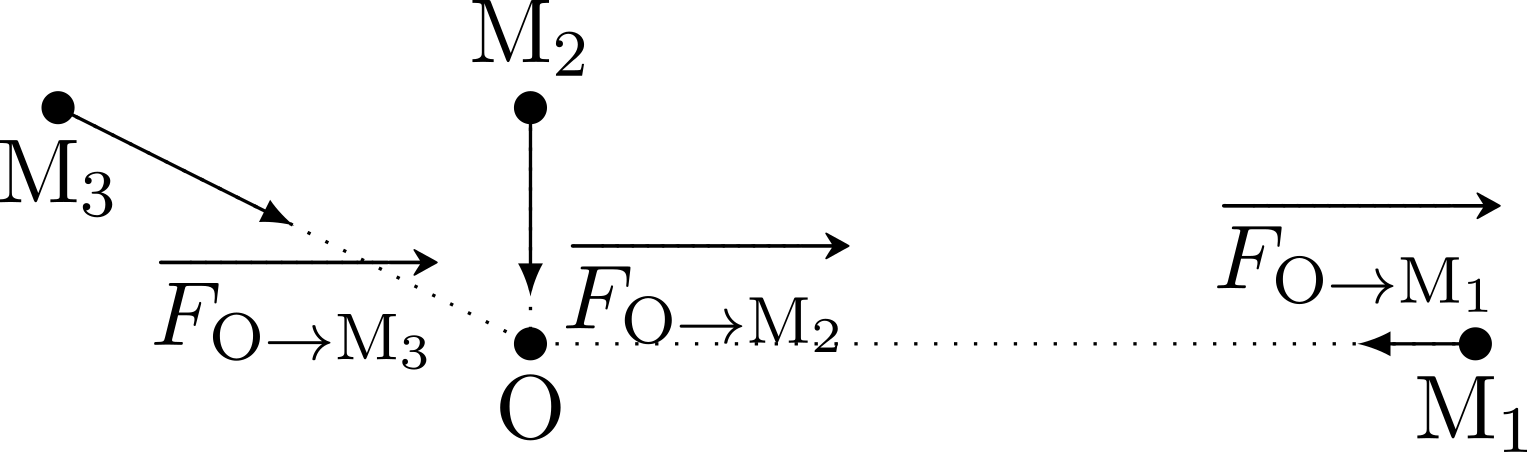
\includegraphics[width=\linewidth]{intro_att}
			\captionof{figure}{Cas attractif}
		\end{center}
		\tcblower
		\begin{center}
			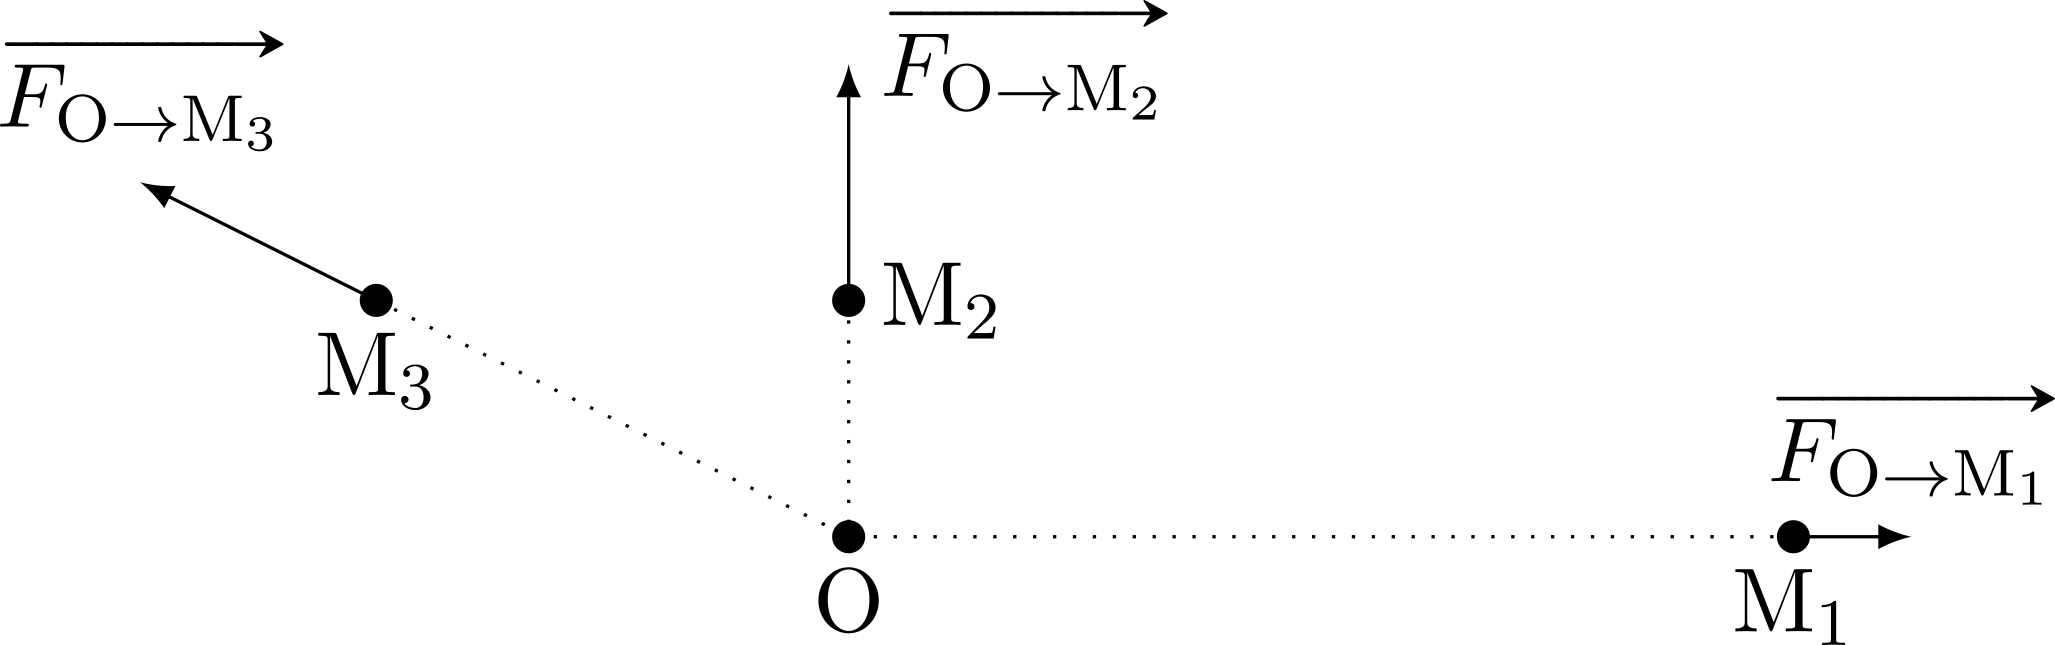
\includegraphics[width=\linewidth]{intro_rep}
			\captionof{figure}{Cas répulsif}
		\end{center}
	\end{isd}
\end{tcb*}
\begin{tcb*}(exem)<lftt>'l'{Forces centrales}
	\begin{itemize}
		\item Force d'attraction gravitationnelle~:
		      \smallbreak
		      \begin{minipage}{0.45\linewidth}
			      \psw{
				      \[\Ff_g = -\Gc \frac{m_\Or m}{r^2}\ur\]
			      }
		      \end{minipage}
		      \hfill
		      \begin{minipage}{0.45\linewidth}
			      \begin{center}
				      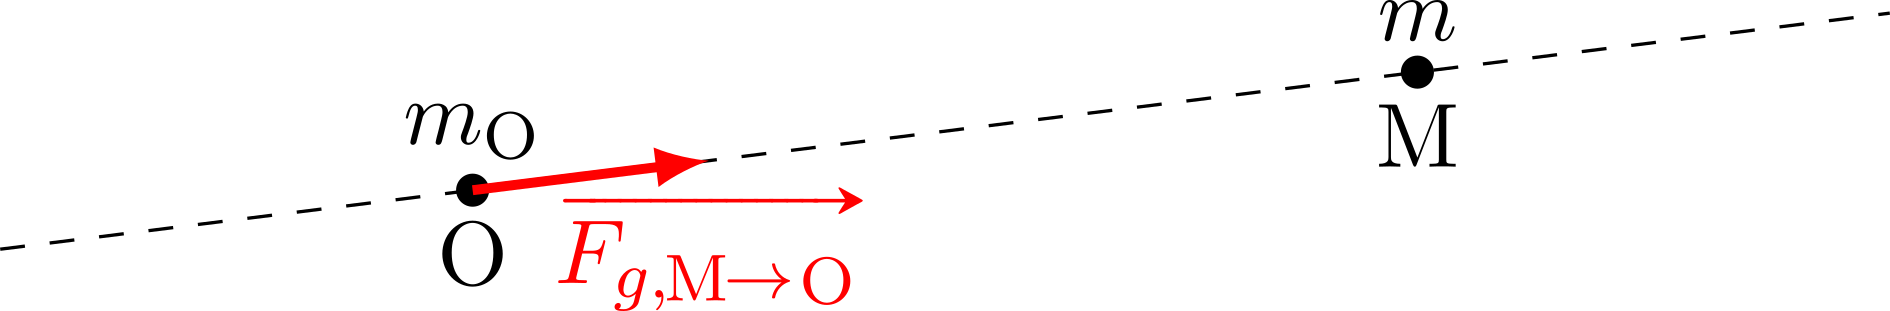
\includegraphics[scale=1]{intro_ex-grav}
			      \end{center}
		      \end{minipage}
		\item Force couloumbienne~: \smallbreak
		      \begin{minipage}{0.45\linewidth}
			      \psw{
				      \[\Ff_e = \frac{1}{4\pi\ep_0} \frac{qq_\Or}{r^2}\ur\]
			      }
		      \end{minipage}
		      \hfill
		      \begin{minipage}{0.45\linewidth}
			      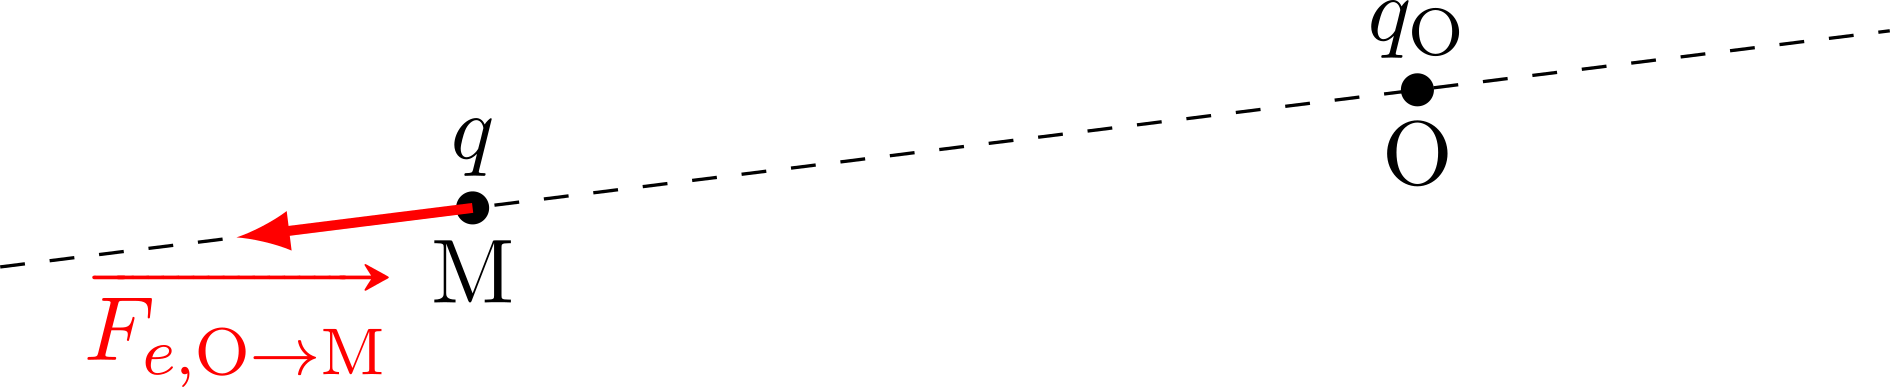
\includegraphics[scale=1]{intro_ex-elec}
		      \end{minipage}
	\end{itemize}
	\vspace{-15pt}
\end{tcb*}

\subsection{Force centrale conservative}
\begin{tcb*}(rapp)<lftt>{Force (centrale) conservative}
	Une force (centrale) est \textbf{conservative} si elle \textbf{dérive d'une
		énergie potentielle}.
\end{tcb*}

\begin{tcb*}(prop){Énergie potentielle d'une force centrale conservative}
	Dans le cas d'une force centrale conservative, en coordonnées
	cylindriques\ftn{Cylindriques ou sphériques} son énergie potentielle ne dépend
	\textbf{que de la distance $r$}~:
	\vspace{-15pt}
	\psw{
		\[
			\boxed{\Ec_{p, \rm centrale}(r,\cancel{\th},\bcancel{z})}
		\]
	}
	\vspace{-15pt}
\end{tcb*}

\begin{tcb*}[breakable](demo)<lftt>{Énergie potentielle d'une FCC}
	Plaçons-nous dans le plan contenant $\OM$ dans un repère polaire centré en O.
	\begin{align*}
		\beforetext{Force centrale $\Ra$}
		\psw{\Ff}
		 & =
		\psw{F(\Mr) \ur}
		\\
		\beforetext{Conservative $\Ra$}
		\psw{\de W(\Ff)} = \psw{-\dd\Ec_p}
		 & \Lra
		\psw{\Ff\cdot\dd{\OM}} = \psw{-\dd{\Ec_p}}
	\end{align*}
	On a alors deux méthodes~:
	\smallbreak
	\begin{isd}[sidebyside align=top]
		\tcbsubtitle{\fatbox{\textbf{Définition de $\dd{\OM}$}}}
		\begin{DispWithArrows*}[format=LrL]
			&
			\Ff \cdot \dd{\OM}
			&=
			\psw{
				F(\Mr) \ur\tikzmark{urg} \cdot \left(
				\dd{r}\ur\tikzmark{urd} +
				r \dd{\th}\ut\tikzmark{ut} +
				\dd{z}\uz\tikzmark{uz}
				\right)
			}
			\\
			&\Lra
			\psw{F(\Mr)\dd{r}}
			&=
			\psw{-\dd{\Ec_p}}
			\\
			&\Lra
			\Aboxed{
				\psw{\dv{\Ec_p}{r}}
				&=
				\psw{-F(\Mr)}
			}
		\end{DispWithArrows*}
		\tcblower
		\tcbsubtitle{\fatbox{\textbf{Utilisation du gradient}}}
		\begin{gather*}
			\Ff = -\gd\Ec_p
			\Lra
			\mqty(\psw{F(\Mr)}\\\psw{0}\\\psw{0})
			=
			\mqty(\DS\psw{-\pdv{\Ec_p}{r}}\\[1em]
			\DS\psw{-\frac{1}{r}\pdv{\Ec_p}{\th}}\\[1em]
			\DS\psw{-\pdv{\Ec_p}{z}}
			)
		\end{gather*}
	\end{isd}
	Ainsi, $\Ec_p$ ne dépend ni de $\th$ ni de $z$, donc dépend uniquement de la
	coordonnée $r$. \hqed
	\tikz[remember picture, overlay]
	\draw[-stealth, transform canvas={yshift=6pt}, color=\sswitch{white}{orchid}]
	(pic cs:urg) to [out=90, in=90]
	node[pos=.2, above left] {$\ur \cdot \ur=1$}
	([shift={(-3pt,3pt)}]pic cs:urd)
	;
	\tikz[remember picture, overlay]
	\draw[-stealth, transform canvas={yshift=6pt}, color=\sswitch{white}{cornflowerblue}]
	(pic cs:urg) to [out=60, in=120]
	node[pos=.8, right] {$\ur \cdot \ut=0$}
	([shift={(-6pt,6pt)}]pic cs:ut)
	;
	\tikz[remember picture, overlay]
	\draw[-stealth, transform canvas={yshift=-3pt}, color=\sswitch{white}{limegreen}]
	(pic cs:urg) to [out=-30, in=-150]
	node[midway, below] {$\ur \cdot \uz=0$}
	([shift={(-3pt,-3pt)}]pic cs:uz)
	;
	% \tikz[remember picture, overlay]
	% \draw[-stealth, transform canvas={yshift=6pt}, color=\sswitch{white}{orange}]
	% (pic cs:DV) to [out=90, in=90] ([shift={(-3pt,6pt)}]pic cs:TP)
	% ;
	% \tikz[remember picture, overlay]
	% \draw[-stealth, transform canvas={yshift=6pt}, color=\sswitch{white}{firebrick}]
	% (pic cs:DV) to [out=90, in=90] ([shift={(-6pt,6pt)}]pic cs:UT)
	% ;
\end{tcb*}

\begin{tcb*}[bld, cnt](impo){Constantes dans les $\Ec_p$}
	Les énergies potentielles sont toujours définies à une constante près, qu'il
	convient de déterminer~!
\end{tcb*}

\begin{tcb*}(appl)<lftt>'l'{Énergies potentielles gravitationnelle et
	électrostatique}
	\begin{itemize}
		\item Interaction gravitationnelle~:
		      \vspace{-15pt}
		      \smallbreak
		      \begin{minipage}{0.45\linewidth}
			      \begin{align*}
				      \pdv{\Ec_{p,\rm g}}{r} & = \psw{\Gc \frac{m_\Or m}{r^2}}
				      \\\Lra
				      \Ec_{p,\rm g}          & = \psw{-\Gc \frac{m_\Or m}{r} + K}
				      \\\Lra
				      \Aboxed{\Ec_{p,\rm g}  & = \psw{-\Gc \frac{m_\Or m}{r}}}
			      \end{align*}
			      en fixant par convention $\Ec_p(+\infty) = 0$.
		      \end{minipage}
		      \hfill
		      \begin{minipage}{0.45\linewidth}
			      \begin{center}
				      \sswitch{
					      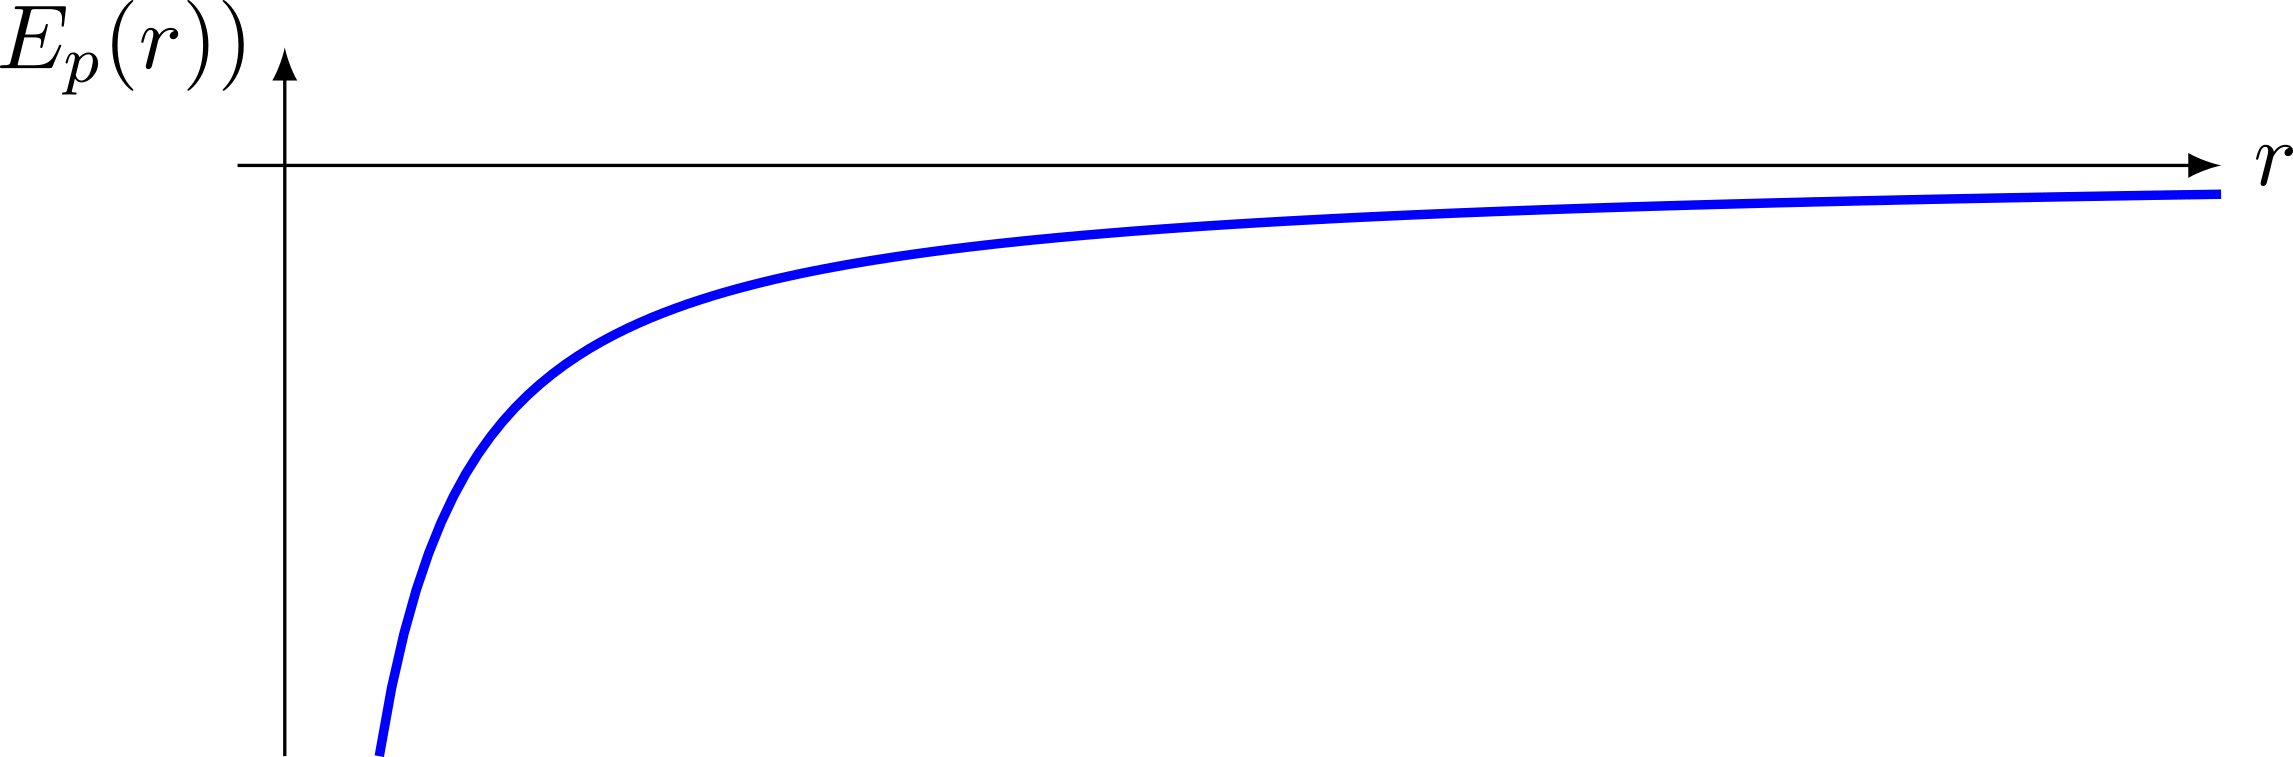
\includegraphics[width=\linewidth, draft=true]{intro_ep-grav}
				      }{
					      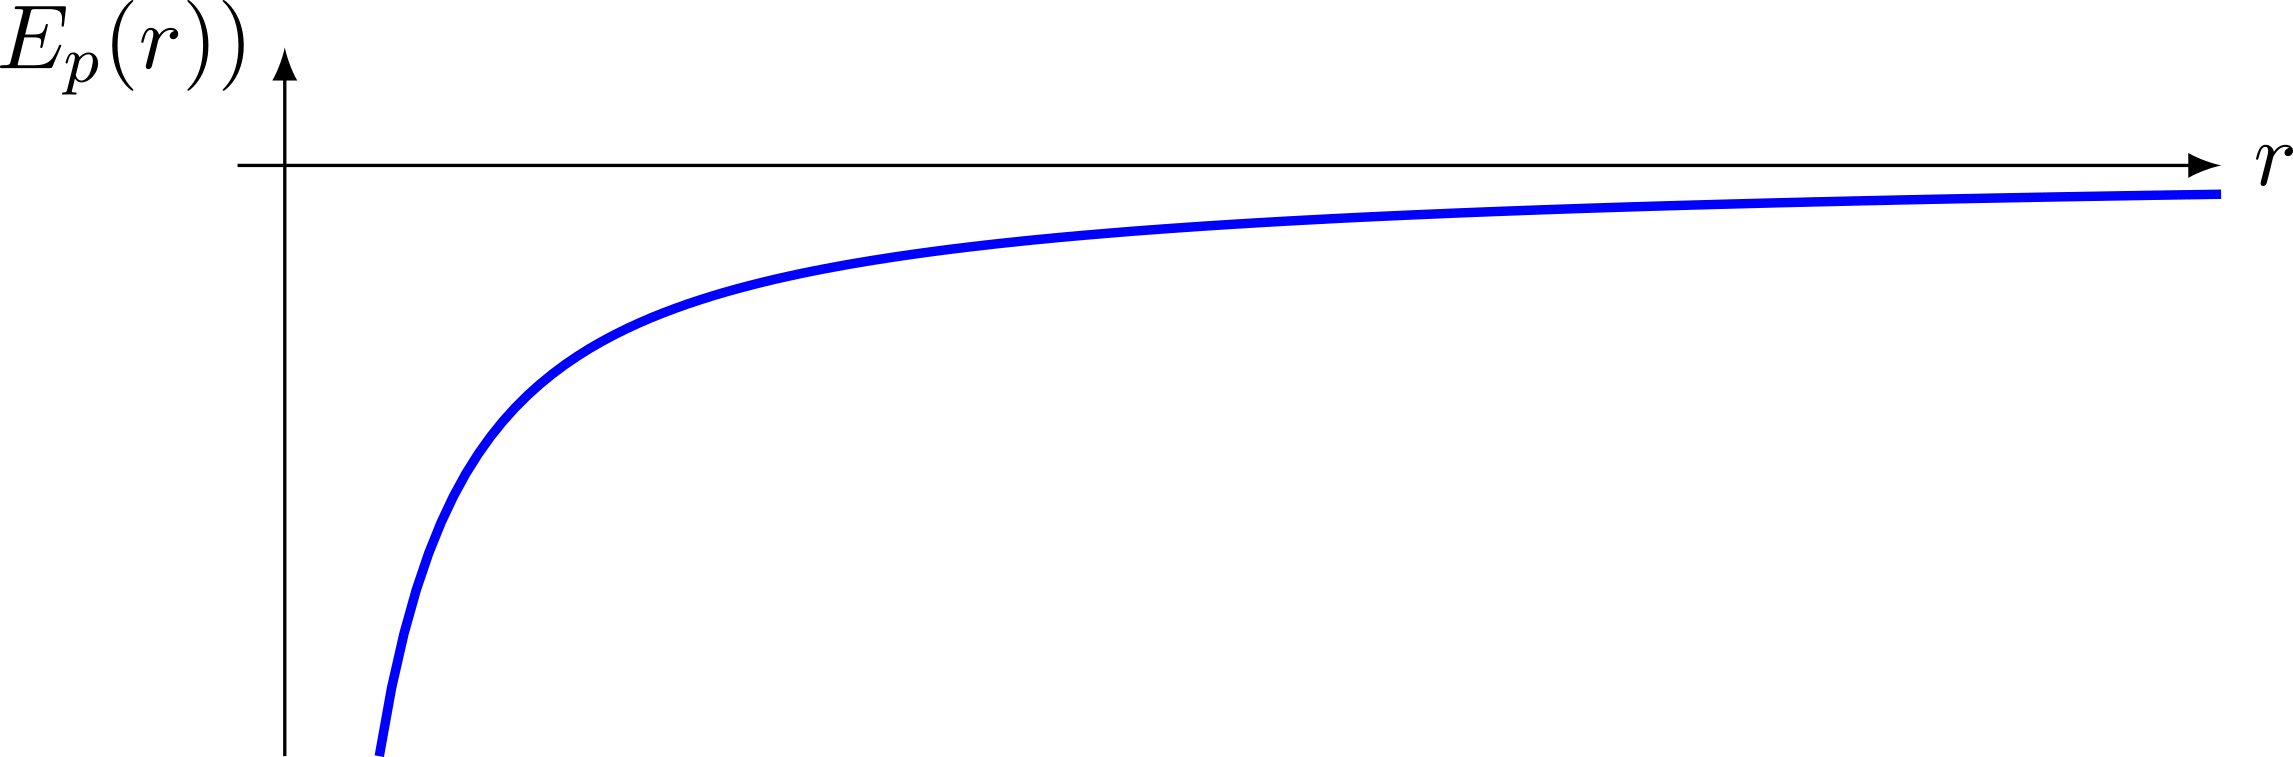
\includegraphics[width=\linewidth]{intro_ep-grav}
				      }
				      \vspace{-15pt}
				      \captionof{figure}{$\Ec_{p,\rm g}(r)$}
			      \end{center}
		      \end{minipage}
		\item Interaction électrostatique~:
		      \vspace{-15pt}
		      \smallbreak
		      \begin{minipage}{0.45\linewidth}
			      \begin{align*}
				      \pdv{\Ec_{p,\rm e}}{r}
				       & =
				      \psw{-\frac{1}{4\pi\ep_0} \frac{qq_\Or}{r^2}}
				      \\\Lra
				      \Ec_{p,\rm e}(r)
				       & =
				      \psw{\frac{1}{4\pi\ep_0} \frac{qq_\Or}{r} + K}
				      \\\Lra
				      \Aboxed{
					      \Ec_{p,\rm e}(r)
				       & =
					      \psw{\frac{1}{4\pi\ep_0} \frac{qq_\Or}{r}}
				      }
			      \end{align*}
			      avec la même convention.
		      \end{minipage}
		      \hfill
		      \begin{minipage}{0.45\linewidth}
			      \begin{center}
				      \sswitch{
					      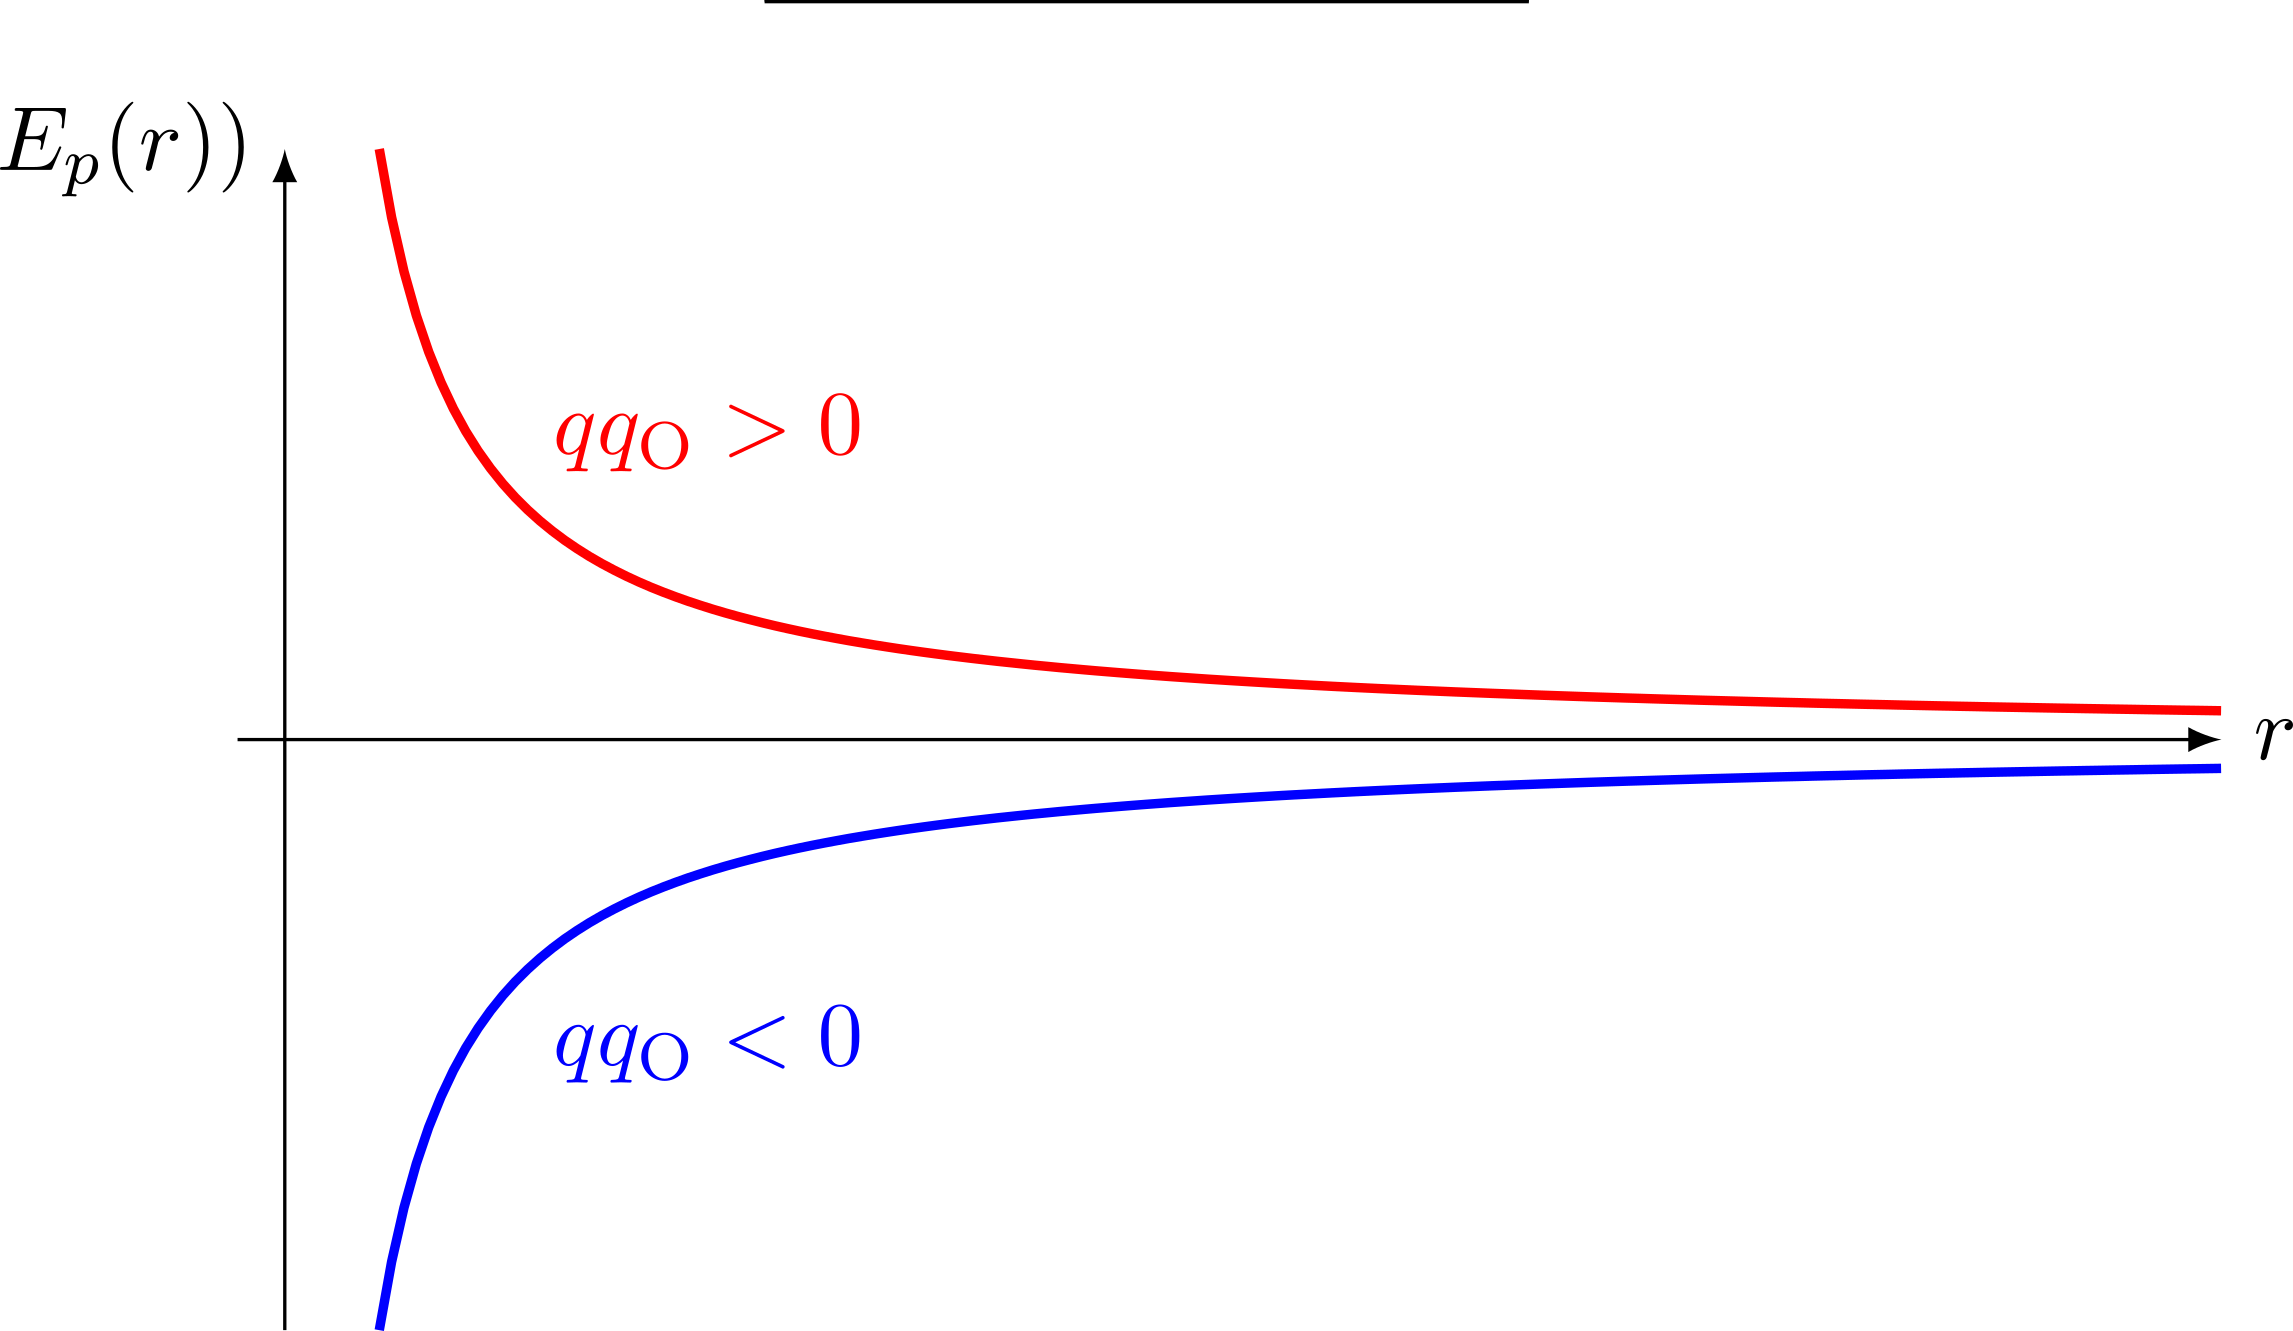
\includegraphics[width=\linewidth, draft=true]{intro_ep-elec}
				      }{
					      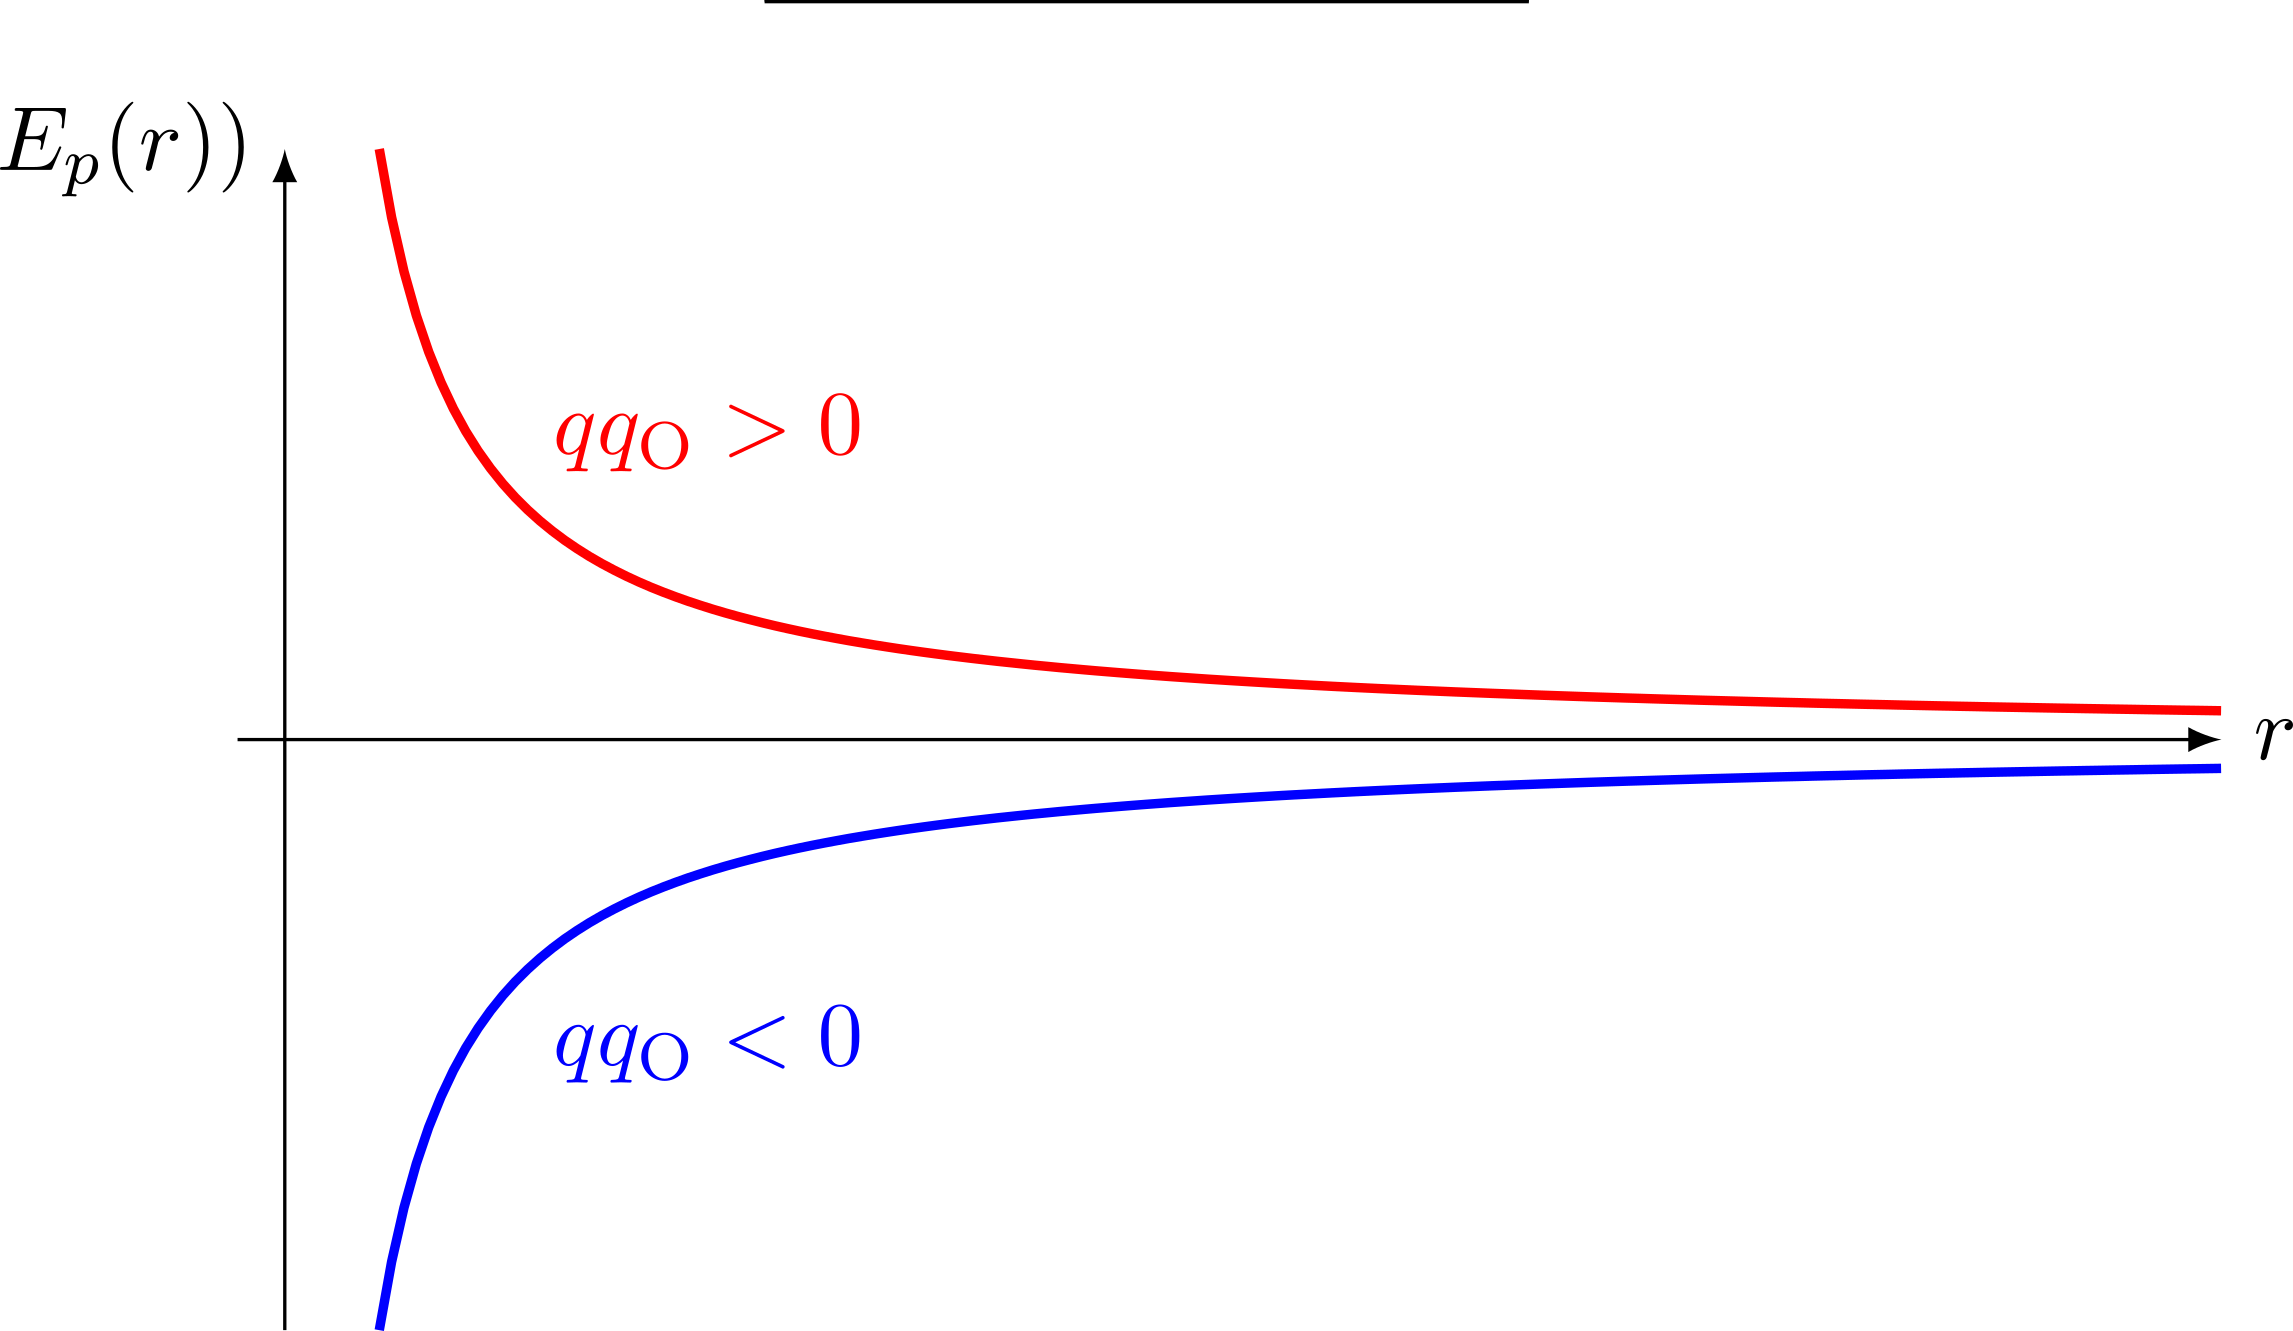
\includegraphics[width=\linewidth]{intro_ep-elec}
				      }
				      \vspace{-15pt}
				      \captionof{figure}{$\Ec_{p,\rm e}(r)$}
			      \end{center}
		      \end{minipage}
	\end{itemize}
	\vspace{-15pt}
\end{tcb*}
\vspace*{-15pt}

\section{Quantités conservées}
\subsection{Conservation du moment cinétique}
\vspace{-5pt}
\begin{tcb*}(prop){Conservation du moment cinétique}
	Pour un point M soumis uniquement à $\Ff$ une force centrale, son moment
	cinétique par rapport au centre de force se conserve~:
	\[
		\psw{
			\boxed{
				\Lcf_\Or(\Mr) = \OM\wedge\pf = \vcte
				\Lra
				\dv{\Lcf_\Or}{t} = \Mcf_\Or(\Ff) = \of
			}
		}
	\]
\end{tcb*}

\begin{tcb*}(demo)<lftt>{Conservation du moment cinétique}
	On considère une force centrale $\Ff$ de centre O. Son moment par rapport à O
	est
	\begin{gather*}
		\psw{\Mcf_\Or(\Ff) = \OM\wedge\Ff = \of}
		\qed
	\end{gather*}
	Si M n'est soumis qu'à $\Ff$, le théorème du moment cinétique en O appliqué à
	M donne bien le résultat.
\end{tcb*}

\subsubsection{Conséquence~: mouvement plan}

\begin{tcb*}[sidebyside](coro){Conservation du moment cinétique~: mouvement
			plan}
	La conservation du moment cinétique d'un point matériel M par rapport à un
	point O fixe dans $\Rc$ implique que le mouvement \textbf{se fait dans le
		plan défini par} $\OM(0)$ et $\vf(0)$.
	\tcblower
	\begin{center}
		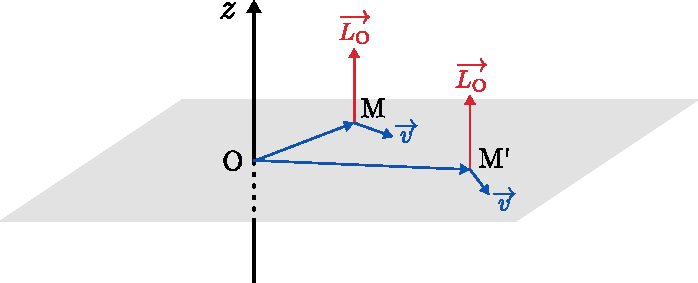
\includegraphics[width=\linewidth]{mvt_plan}
		\captionof{figure}{$\protect\Lcf_{\Or} = \protect\vcte \Ra$ mouvement plan}
	\end{center}
\end{tcb*}

\begin{tcb*}(demo)<lftt>{Conservation du moment cinétique~: mouvement
			plan}
	Soit $\uz$ la direction initale du moment cinétique, c'est-à-dire
	\psw{
		\[\Lcf(0) = \OM(0)\wedge m\vf(0) = \Lc_0 \uz\]
	}
	$\uz$ définit donc une direction perpendiculaire à $\OM(0)$ et $\vf(0)$. Or,
	comme $\Lcf$ se conserve, on a
	\[\Lcf(t) = \Lcf(0) \Lra \psw{\OM(t)\wedge m\vf(t) = \Lc_0\uz}\]
	donc $\OM$ et $\vf$ \textbf{restent orthogonaux} à $\uz$. Autrement dit,
	\textbf{le mouvement reste dans le plan $\perp \text{à} \uz$ passant par O}.
	\hqed
\end{tcb*}

\begin{tcb*}(rema)<lftt>'l'{Nullité du moment cinétique}
	Si $\OM(0)$ et $\vf(0)$ sont colinéaires, alors $\Lcf(0)$ est nul, et reste
	donc nul à tout instant~: $\OM$ et $\vf$ restent colinéaires, et le
	mouvement est alors simplement rectiligne.
\end{tcb*}
\vspace{-15pt}

\subsubsection{Conséquence~: loi des aires}
% On a vu dans le chapitre précédent que la norme du moment d'une force décrivait
% l'aire du parallélépipède formé par $\OM$ et $\Ff\ind{plan}$. On peut réfléchir
% de la même manière avec le moment cinétique. Pour ça, un tout petit peu de
% géométrie.

% \begin{tcb*}(prop){Aire d'un triangle}
% 	\begin{minipage}{0.80\linewidth}
% 		L'aire d'un triangle ABC peut être calculée à partir de la formule~:
% 		\[
%       \Ac =
%       \frac{1}{2}\norm{\ABf\wedge\vvr{AC}} =
%       \frac{1}{2}\norm{\ABf}\norm{\vvr{AC}}\sin(\th)
%     \]
%     C'est la moitié du parallélograme formé par $\ABf$ et $\vvr{AC}$.
% 	\end{minipage}
% 	\hfill
% 	\begin{minipage}{0.19\linewidth}
% 		\begin{center}
% 			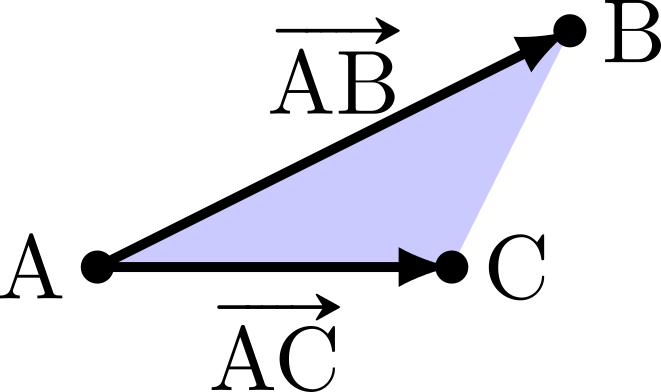
\includegraphics[scale=1]{aire_tri}
% 		\end{center}
% 	\end{minipage}
% \end{tcb*}

\begin{tcb*}[sidebyside](coro){Conservation du moment cinétique~: loi des aires}
	L'aire balayée $\dd{\Ac}$ par le vecteur $\OM$ en un temps $\dd{t}$ est
	constante~; autrement dit
	\begin{framed}
		\setlength{\topsep}{0pt}
		\begin{center}
			Pour un point M soumis uniquement à une force centrale, des aires égales
			sont balayées pendant un temps égal.
		\end{center}
	\end{framed}
	\tcblower
	\begin{center}
		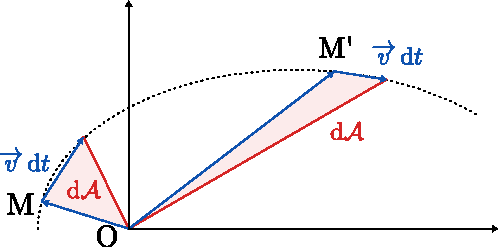
\includegraphics[width=\linewidth]{kepler_2-aire}
		\captionof{figure}{Loi des aires.}
	\end{center}
\end{tcb*}

En effet, avec un schéma on peut la relier au moment cinétique~:
\begin{tcb*}[sidebyside](demo)<lftt>{Conservation du moment cinétique~: loi des
  aires}
	La norme du moment cinétique quantifie l'aire balayée $\dd{\Ac}$ pendant un
	temps $\dd{t}$~:
	\begin{align*}
		\dd{\Ac}            & = \psw{\frac{1}{2}\norm{\OM \wedge \vf \dd{t}}}
		\\\Lra
		\dd{\Ac}            & = \psw{\frac{1}{2}\norm{\OM \wedge m \vf} \frac{\dd{t}}{m}}
		\\\Lra
		\Aboxed{\dv{\Ac}{t} & = \psw{\frac{\norm{\Lcf_{\Or}}}{2m} = \cte}}
		\qed
	\end{align*}
	\tcblower
	% TODO: Remplacer \Gamma par \Lcf
	\begin{center}
		\sswitch{
			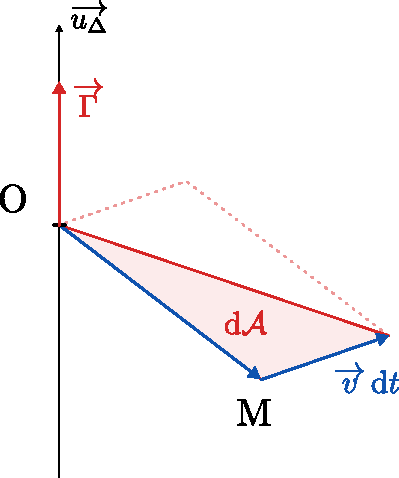
\includegraphics[scale=.6, draft=true]{dAmomcin}
		}{
			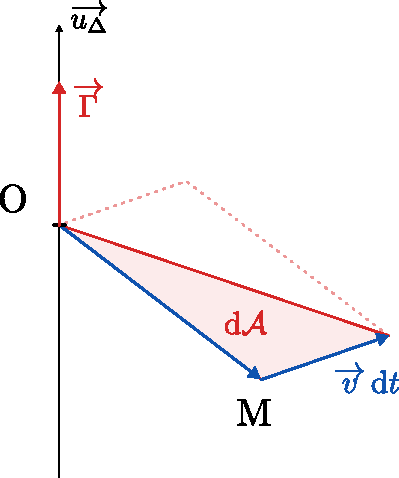
\includegraphics[scale=.6]{dAmomcin}
		}
		\captionof{figure}{Moment cinétique et aire balayée.}
	\end{center}
\end{tcb*}

% Ainsi, en prenant M comme origine du repère et correspondant à A dans la formule
% proposée, on peut déterminer l'aire dite «~balayée~» par le point M autour de O
% pendant un temps $\dt$, tel que le mouvement soit suffisamment court pour
% décrire le triangle OM$(t)$M$(t+\dt)$~:
% \begin{align*}
% 	\dd{\Ac}            & = \frac{1}{2}\norm{\vv{\Mr(t)\Or}\wedge\vv{\Mr(t)\Mr(t+\dt)}}
% 	\shortintertext{Or, par construction on a $\vv{\Mr(t)\Mr(t+\dt)} = \vf\dt$,
% 		d'où}
% 	\dd{\Ac}            & = \frac{1}{2}\norm{-\OM(t)\wedge\vf}\dt
% 	\\\Lra
% 	\Aboxed{\dv{\Ac}{t} & = \frac{\norm{\Lcf_\Or}}{2m} = \cte}
% \end{align*}
% ce qui est la deuxième loi de \textsc{Kepler}, dont on rediscutera plus tard~:
% \begin{tcb*}(prop){Deuxième loi de \textsc{Kepler}}
% 	\begin{minipage}{0.44\linewidth}
% 		Pour un point M soumis uniquement à une force centrale, des aires égales
% 		sont balayées pendant un temps égal.
% 	\end{minipage}
% 	\hfill
% 	\begin{minipage}{0.55\linewidth}
% 		\begin{center}
% 			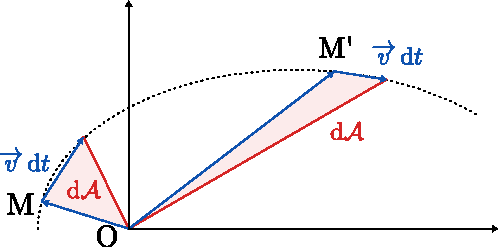
\includegraphics[scale=1]{kepler_2-aire}
% 		\end{center}
% 	\end{minipage}
% \end{tcb*}

\subsubsection{Conséquence~: constante des aires}
\begin{tcb*}(coro){Conservation du moment cinétique~: constante des aires}
	On appelle \textbf{constante des aires} la grandeur conservée
	\psw{
		\[
			\boxed{C = r^{2}\tp} \Lra \dv{\Ac}{t} = \frac{C}{2}
		\]
	}
	Elle est donc constante au cours du mouvement, i.e. $\tp$ est de \textbf{signe
		constant} et la rotation ne s'inverse jamais.
\end{tcb*}
\begin{tcb*}(demo)<lftt>{Conservation du moment cinétique~: constante des aires}
	Le mouvement étant plan, on peut se placer en coordonnées polaires~:
	\begin{gather*}
		\left\{
		\begin{aligned}
			\OM & = \psw{r\ur}            \\
			\vf & = \psw{\rp\ur + r\w\ut}
		\end{aligned}
		\right.
		\quad\Ra\quad
		\Lcf_{\Or} = \psw{(r\ur)\wedge m(\rp\ur+r\tp\ut) = mr^2\tp\uz}
	\end{gather*}
	\begin{isd}
		\vspace{-15pt}
		\begin{gather*}
			\beforetext{Or}
			\psw{\norm{\Lcf_{\Or}} = m \underbracket[1pt]{r^{2}\tp}_{=C} = \cte}
			\\\Lra
			\psw{\boxed{C = \frac{\norm{\Lcf_{\Or}}}{m}}}
		\end{gather*}
		\tcblower
		\vspace{-15pt}
		\begin{gather*}
			\beforetext{De plus}
			\psw{\dv{\Ac}{t} = \frac{\norm{\Lcf_{\Or}}}{2m}}
			\\\Lra
			\psw{\boxed{\dv{\Ac}{t} = \frac{C}{2}}}
			\qed
		\end{gather*}
	\end{isd}
\end{tcb*}

% Reprenons les coordonnées cylindriques
% centrées sur O, avec $\uz \perp \Lcf_0$ donc perpendiculaire au mouvement. On a
% \begin{align*}
% 	\OM      & = r\ur
% 	\\\Ra
% 	\vf      & = \rp\ur + r\tp\ut
% 	\\\Ra
% 	\Lcf_\Or & = \OM\wedge m\vf = mr^2\tp
% \end{align*}
% Ainsi,
% \begin{tcb*}(defi){Constante des aires, heart}
% 	La \textbf{constante des aires} est la grandeur
% 	\[C = r^2\tp\]
% 	et est une quantité constante au cours du mouvement. Notamment, $\tp$ est de
% 	\textbf{signe constant}, et la rotation se fait toujours dans le même sens.
% \end{tcb*}

\subsection{Conservation de l'énergie mécanique}

\begin{tcb*}(prop){Énergie potentielle effective}
	L'énergie mécanique d'un point matériel M soumis à une force centrale
	conservative est constante, et peut se mettre sous la forme
	\[
		\psw{
			\Ec_m = \frac{1}{2}m \rp^{2} + \Ec_{p,\rm eff}(r) = \cte
		}
		\qqav
		\psw{
			\boxed{\Ec_{p,\rm eff} = \frac{1}{2}m \frac{C^2}{r^2} + \Ec_p(r)}
		}
	\]
\end{tcb*}

\begin{tcb*}(demo)<lftt>{Énergie potentielle effective}
	Toujours pour M soumis uniquement à une force centrale conservative,
	\smallbreak
	\begin{isd}[righthand ratio=.4]
		\begin{align*}
			\psw{\dv{\Ec_m}{t} \overset{\rm TEM}{=} 0}
			\quad & \text{et} \quad
			\Ec_m = \Ec_c + \Ec_p
			\\
			\beforetext{Or}
			\psw{v^2   = \rp^2 + (r\tp)^2}
			      & \Ra
			\psw{\Ec_m = \frac{1}{2}m\rp^2 + \frac{1}{2}mr^2\tp^2 + \Ec_p}
		\end{align*}
		\tcblower
		or $\boxed{\psw{\tp = C/r^2}}$ d'où
		\begin{gather*}
			\boxed{
				\psw{
					\Ec_m = \frac{1}{2}m\rp^2 +
					\underbracket[1pt]{\frac{1}{2}m \frac{C^2}{r^2}+\Ec_p}_{\Ec_{p,\rm eff}}
				}
			}
			\qed
		\end{gather*}
	\end{isd}
\end{tcb*}

\begin{tcb*}(inte)<lftt>{Énergie potentielle effective}
	L'énergie potentielle effective permet de se ramener à l'étude d'une seule
	dimension, ici $r$ la distance au centre de force, plutôt que d'utiliser à la
	fois $r$ et $\th$, en considérant $\Ec_{p,\rm eff}$ comme l'énergie potentielle
	du système et $\frac{1}{2}m \rp^{2}$ son énergie cinétique.
\end{tcb*}

\section{Champs de force newtoniens}
\subsection{Cas général}
\begin{tcb*}(defi){Force newtonienne}
	\begin{isd}
		Force centrale est dite \textbf{newtonienne}~:
		\psw{
			\[\boxed{\Ff = -\frac{k}{r^2}\ur}\]
		}
		\vspace{-15pt}
		\tcblower
		L'énergie potentielle associée est alors
		\psw{\[\boxed{\Ec_p(r) = -\frac{k}{r}}\]}
		\vspace{-15pt}
	\end{isd}
	On observe alors
	\begin{tasks}[label=$\diamond$](2)
		\task $k>0 \Ra$ \psw{force attractive}~;
		\task $k<0 \Ra$ \psw{force répulsive}.
	\end{tasks}
	et l'énergie potentielle effective est
	\[\boxed{\psw{\Ec_{p,\rm eff} = \frac{1}{2}m\frac{C^2}{r^2} - \frac{k}{r}}}\]
\end{tcb*}

\begin{tcb*}(exem)<lftt>'l'{Cas classiques}
	\begin{itemize}
		\item Pour l'interaction gravitationnelle, $k = \psw{\Gc m_\Or m}$~;
		\item Pour l'interaction électrostatique, $k = \psw{-q_\Or q/4\pi\ep_0}$.
	\end{itemize}
\end{tcb*}

Nous allons maintenant étudier les différentes trajectoires possibles en
fonction de l'énergie mécanique totale et de cette énergie potentielle
effective.

\subsection{Cas attractif}
\subsubsection{Étude mathématique}
Analysons la fonction $\Ec_{p,\rm eff}(r)$~:
\begin{tasks}[label=$\diamond$](3)
	\task $\DS \lim_{r\to0} \Ec_{p,\rm eff}(r) = +\infty$~;
	\task $\DS \lim_{r\to+\infty} \Ec_{p,\rm eff}(r) = 0$~;
	\task $\Ec_{p,\rm eff}$ présente un minimum.
\end{tasks}
\noindent
\begin{isd}
	En effet,
	\begin{DispWithArrows*}[format=CrCL]
		&
		\eval{\dv{\Ec_{p,\rm eff}}{r}}_{r\ind{min}}
		& = & 0
		\\
		\Lra
		&
		\psw{\frac{1}{2}m\left(-2 \frac{C^2}{r\ind{min}^3}\right) +
			\frac{k}{r\ind{min}^2}}
		& = & 0
		\\
		\Lra &
		\psw{-mC^2 + kr\ind{min}}
		& = & 0
		\\
		\Lra &
		\psw{r\ind{min}} & = & \psw{\frac{mC^2}{k}}
		\\
		\text{Ainsi}
		&
		\Ec_{p,\rm eff}(r_{\min}) & = & \psw{-\frac{k^2}{2mC^2} = - \Ec_0}
	\end{DispWithArrows*}
	\tcblower
	\begin{center}
		\sswitch{
			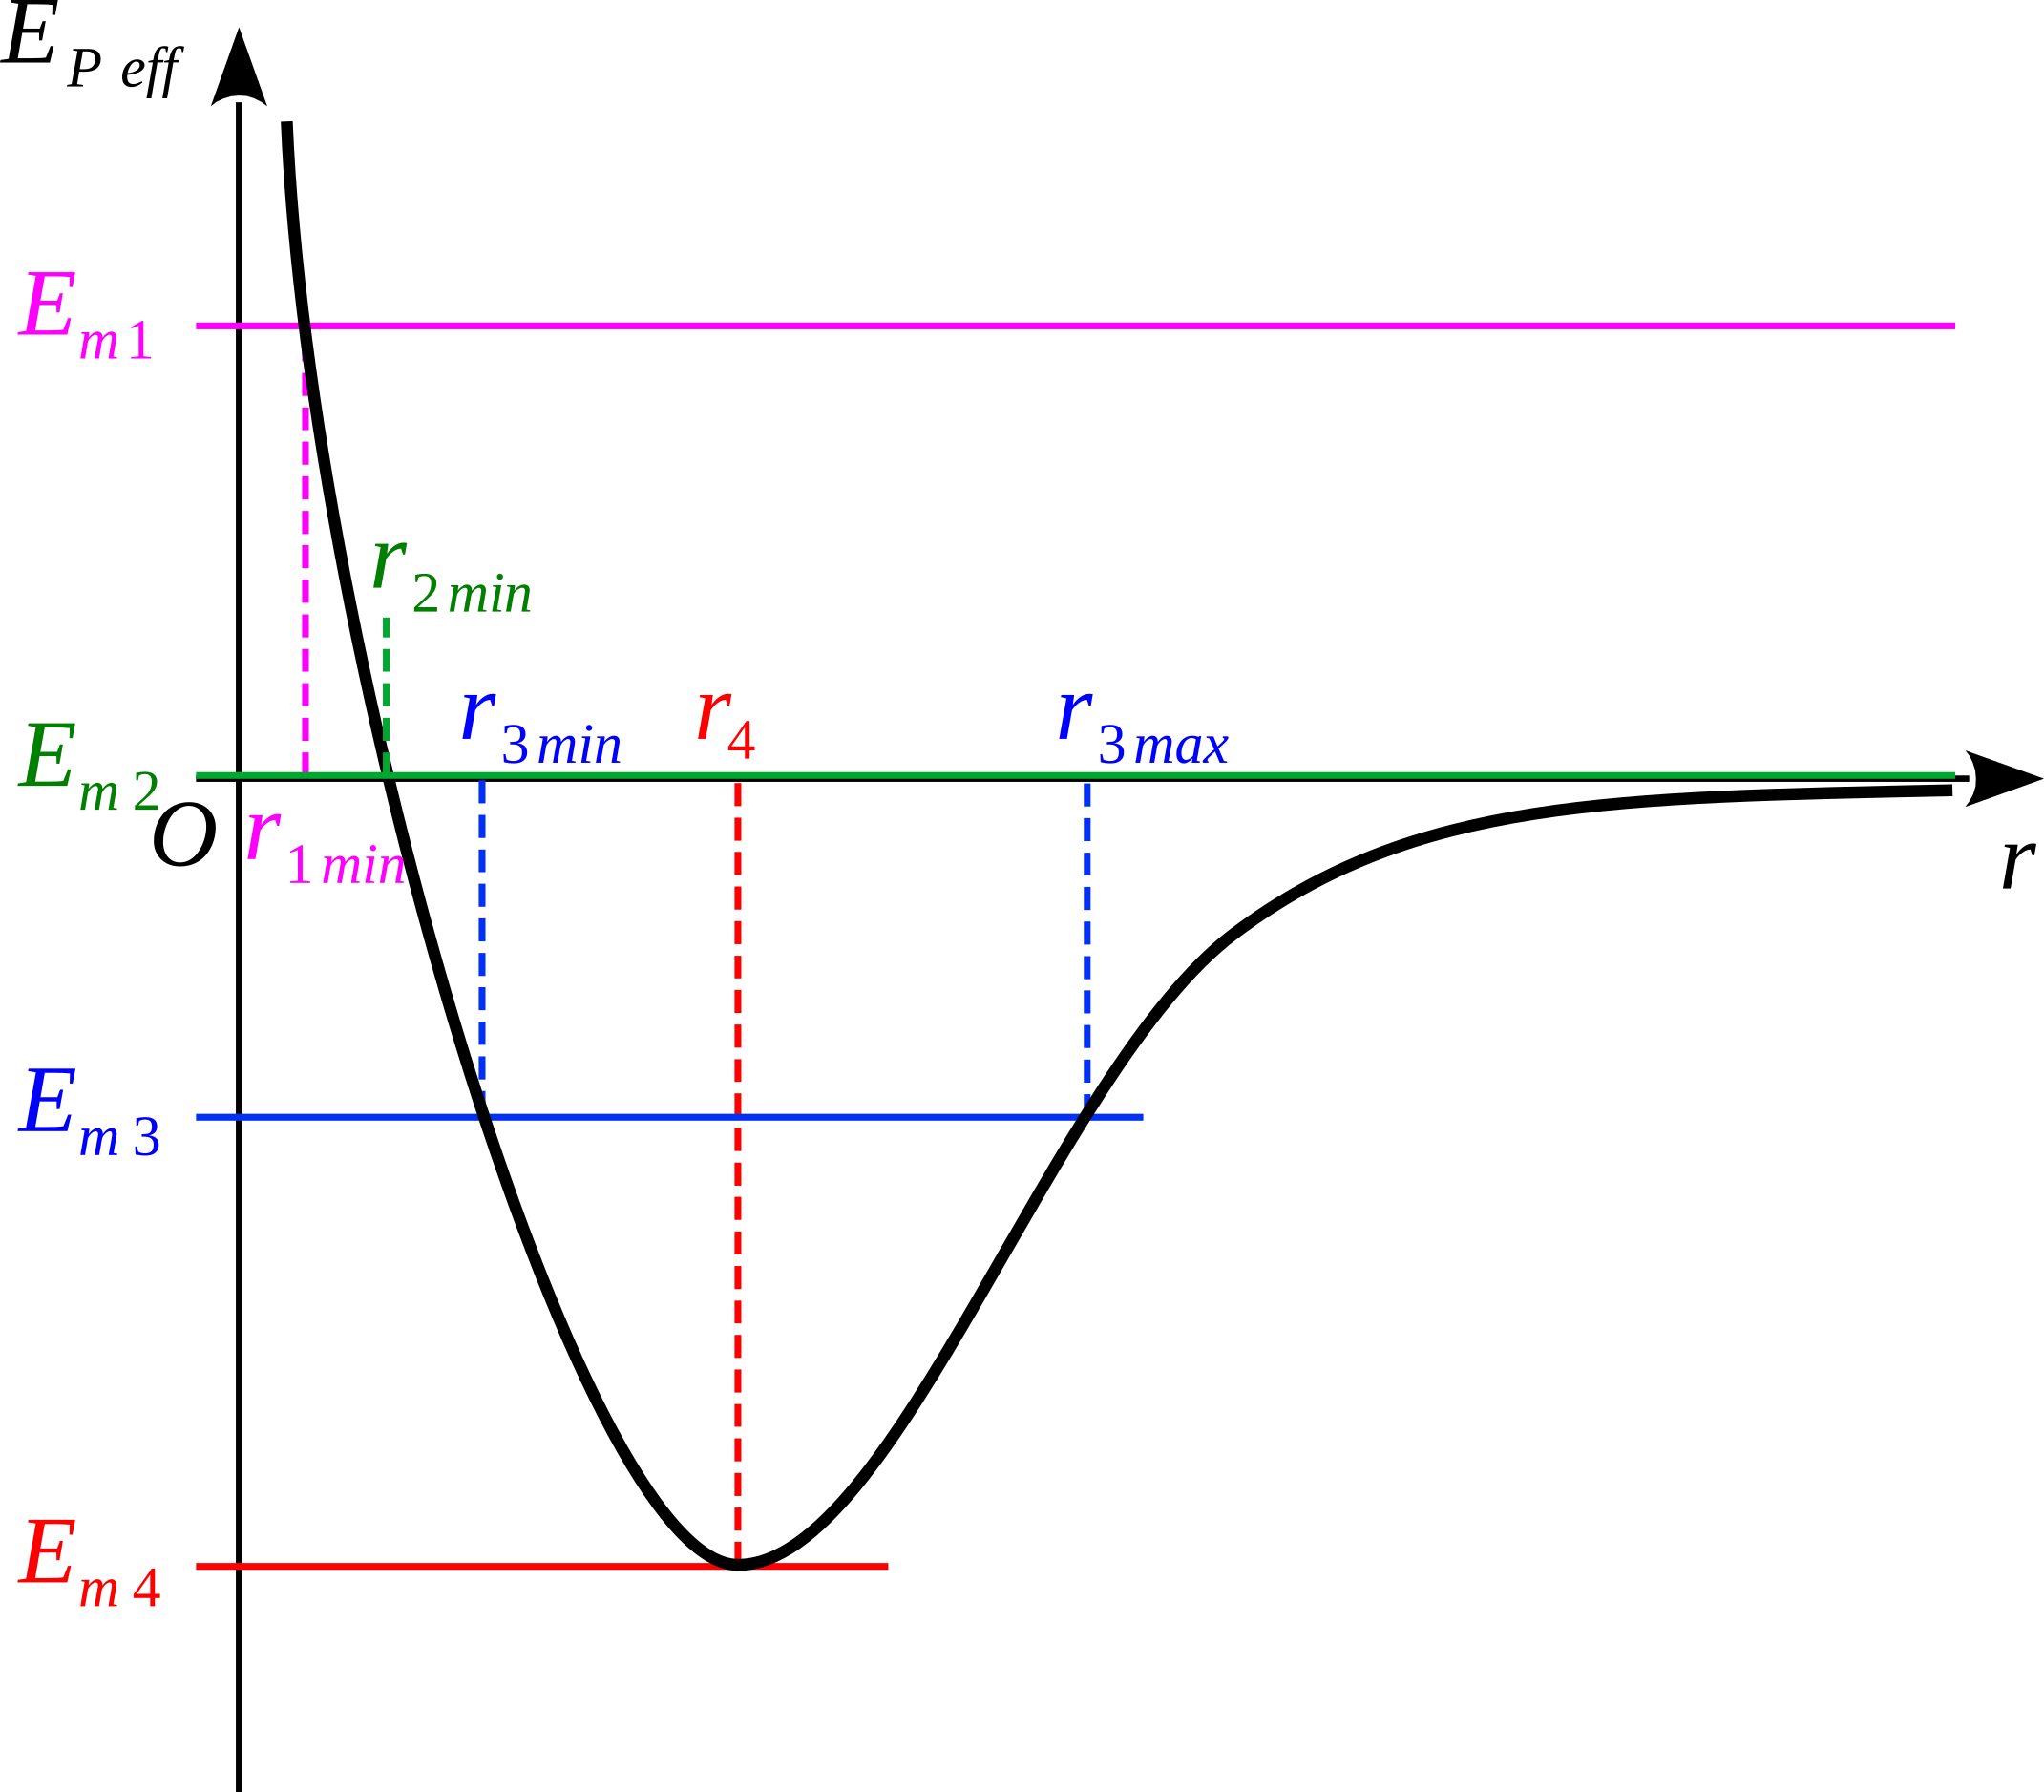
\includegraphics[width=.8\linewidth,draft=true]{ep_eff-att_color}
		}{
			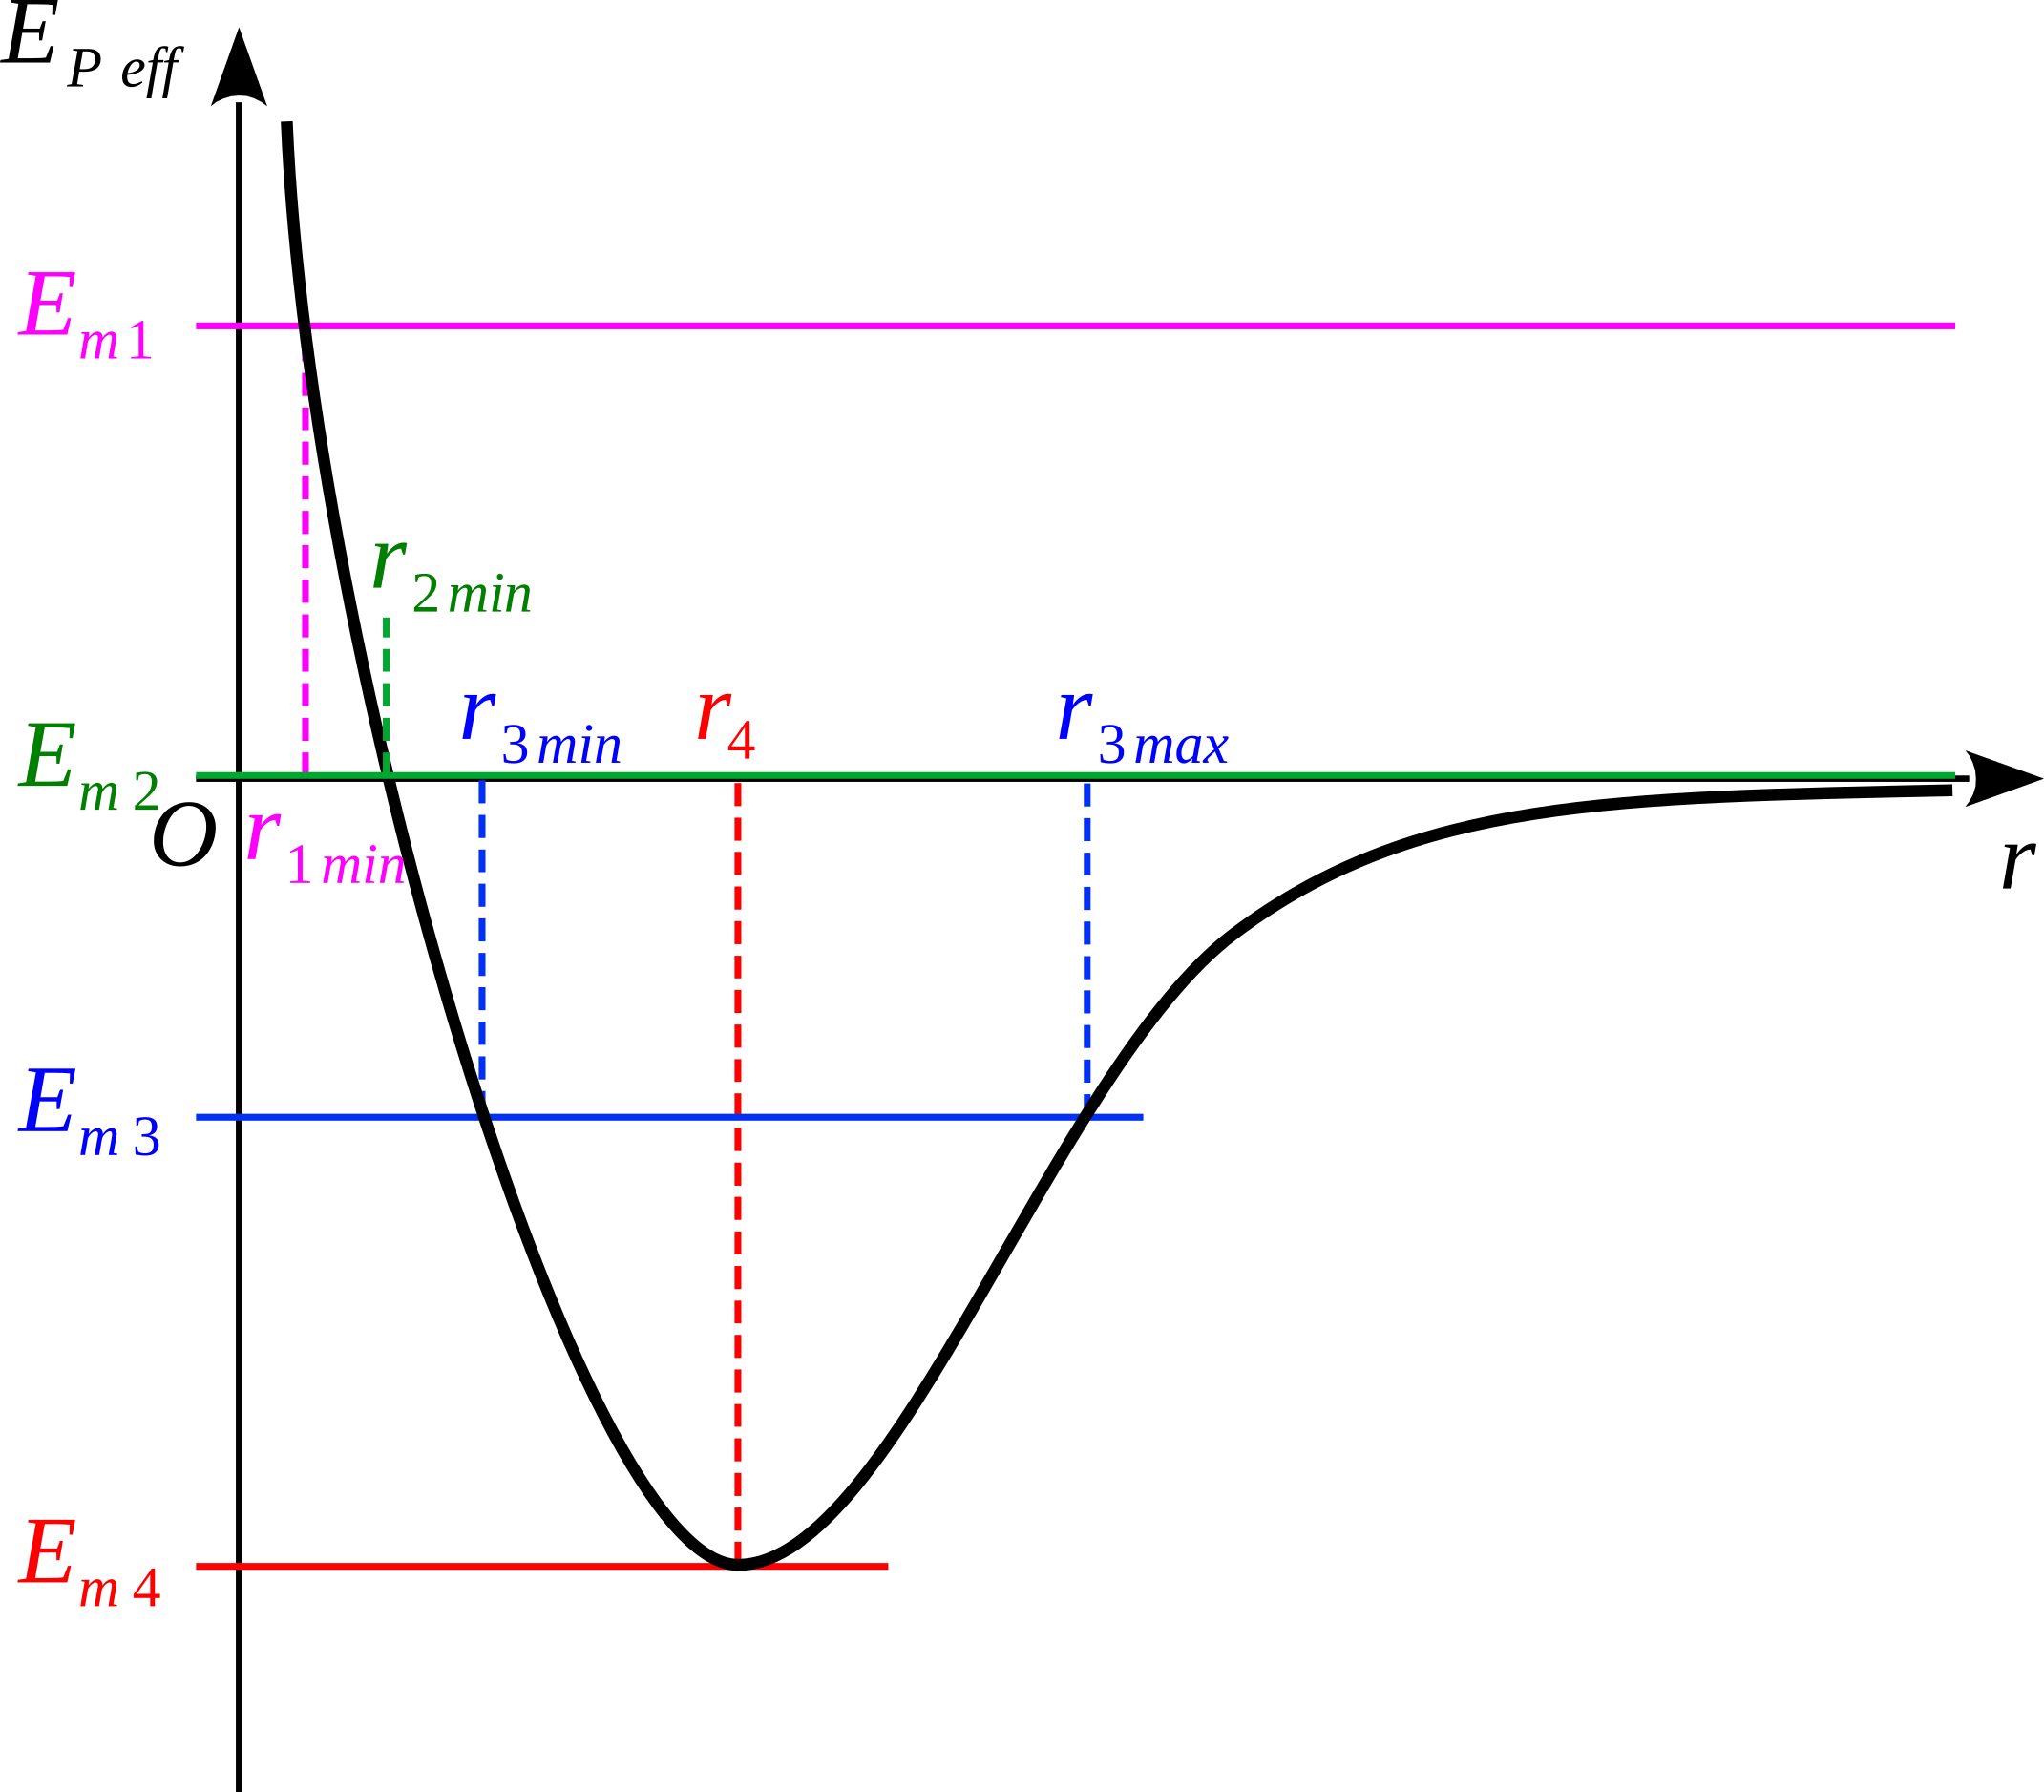
\includegraphics[width=.8\linewidth]{ep_eff-att_color}
		}
		\captionof{figure}{$\Ec_{p,\rm eff}$ cas attractifs.}
	\end{center}
\end{isd}

\subsubsection{Étude des trajectoires}
\label{ssec:trajatt}

Comme $\Ec_m = \frac{1}{2}m\rp^2 + \Ec_{p,\rm eff}$, on a forcément
$\boxed{\Ec_{p,\rm eff} < \Ec_m}$. Ainsi, selon la valeur de $\Ec_m$ par rapport
à $\Ec_{p,\rm eff}(r)$, le système aura différentes trajectoires, toutes ayant O
comme foyer ou centre~:
\begin{itemize}
	\item $\Ec_m \geq 0$~:
	      \psw{
		      la trajectoire n'est \textbf{pas bornée}, on aura
		      donc un état de \textbf{diffusion} avec deux valeurs minimales possibles
		      et deux trajectoires possibles, hyperbolique et parabolique~;
	      }
	\item $\Ec_m < 0$~:
	      \psw{
		      la trajectoire \textbf{est bornée}, on aura donc un état \textbf{lié}
		      avec deux valeurs extrêmes différentes pour la trajectoire elliptique ou
		      une seule, $r_{\min}$, pour la trajectoire circulaire.
	      }
\end{itemize}

% \begin{table}[h]
%     \begin{tabularx}{\linewidth}{lYY}
%         \toprule
%         \multirow{2}{*}[-3pt]{Caractéristique} &
%         \multicolumn{2}{c}{Type de mouvement}
%         \\\cmidrule(lr){2-3}
%         &
%         \textbf{Diffusion} $\Ec_m \geq 0$
%         &
%         \textbf{Lié} $\Ec_m < 0$
%         \\\midrule
%         Valeur de $\Ec_m$ &
%         $0 < \Ec_m < \infty$ &
%         $-\Ec_0 < \Ec_m < 0$
%         \\
%         Graphique &
%         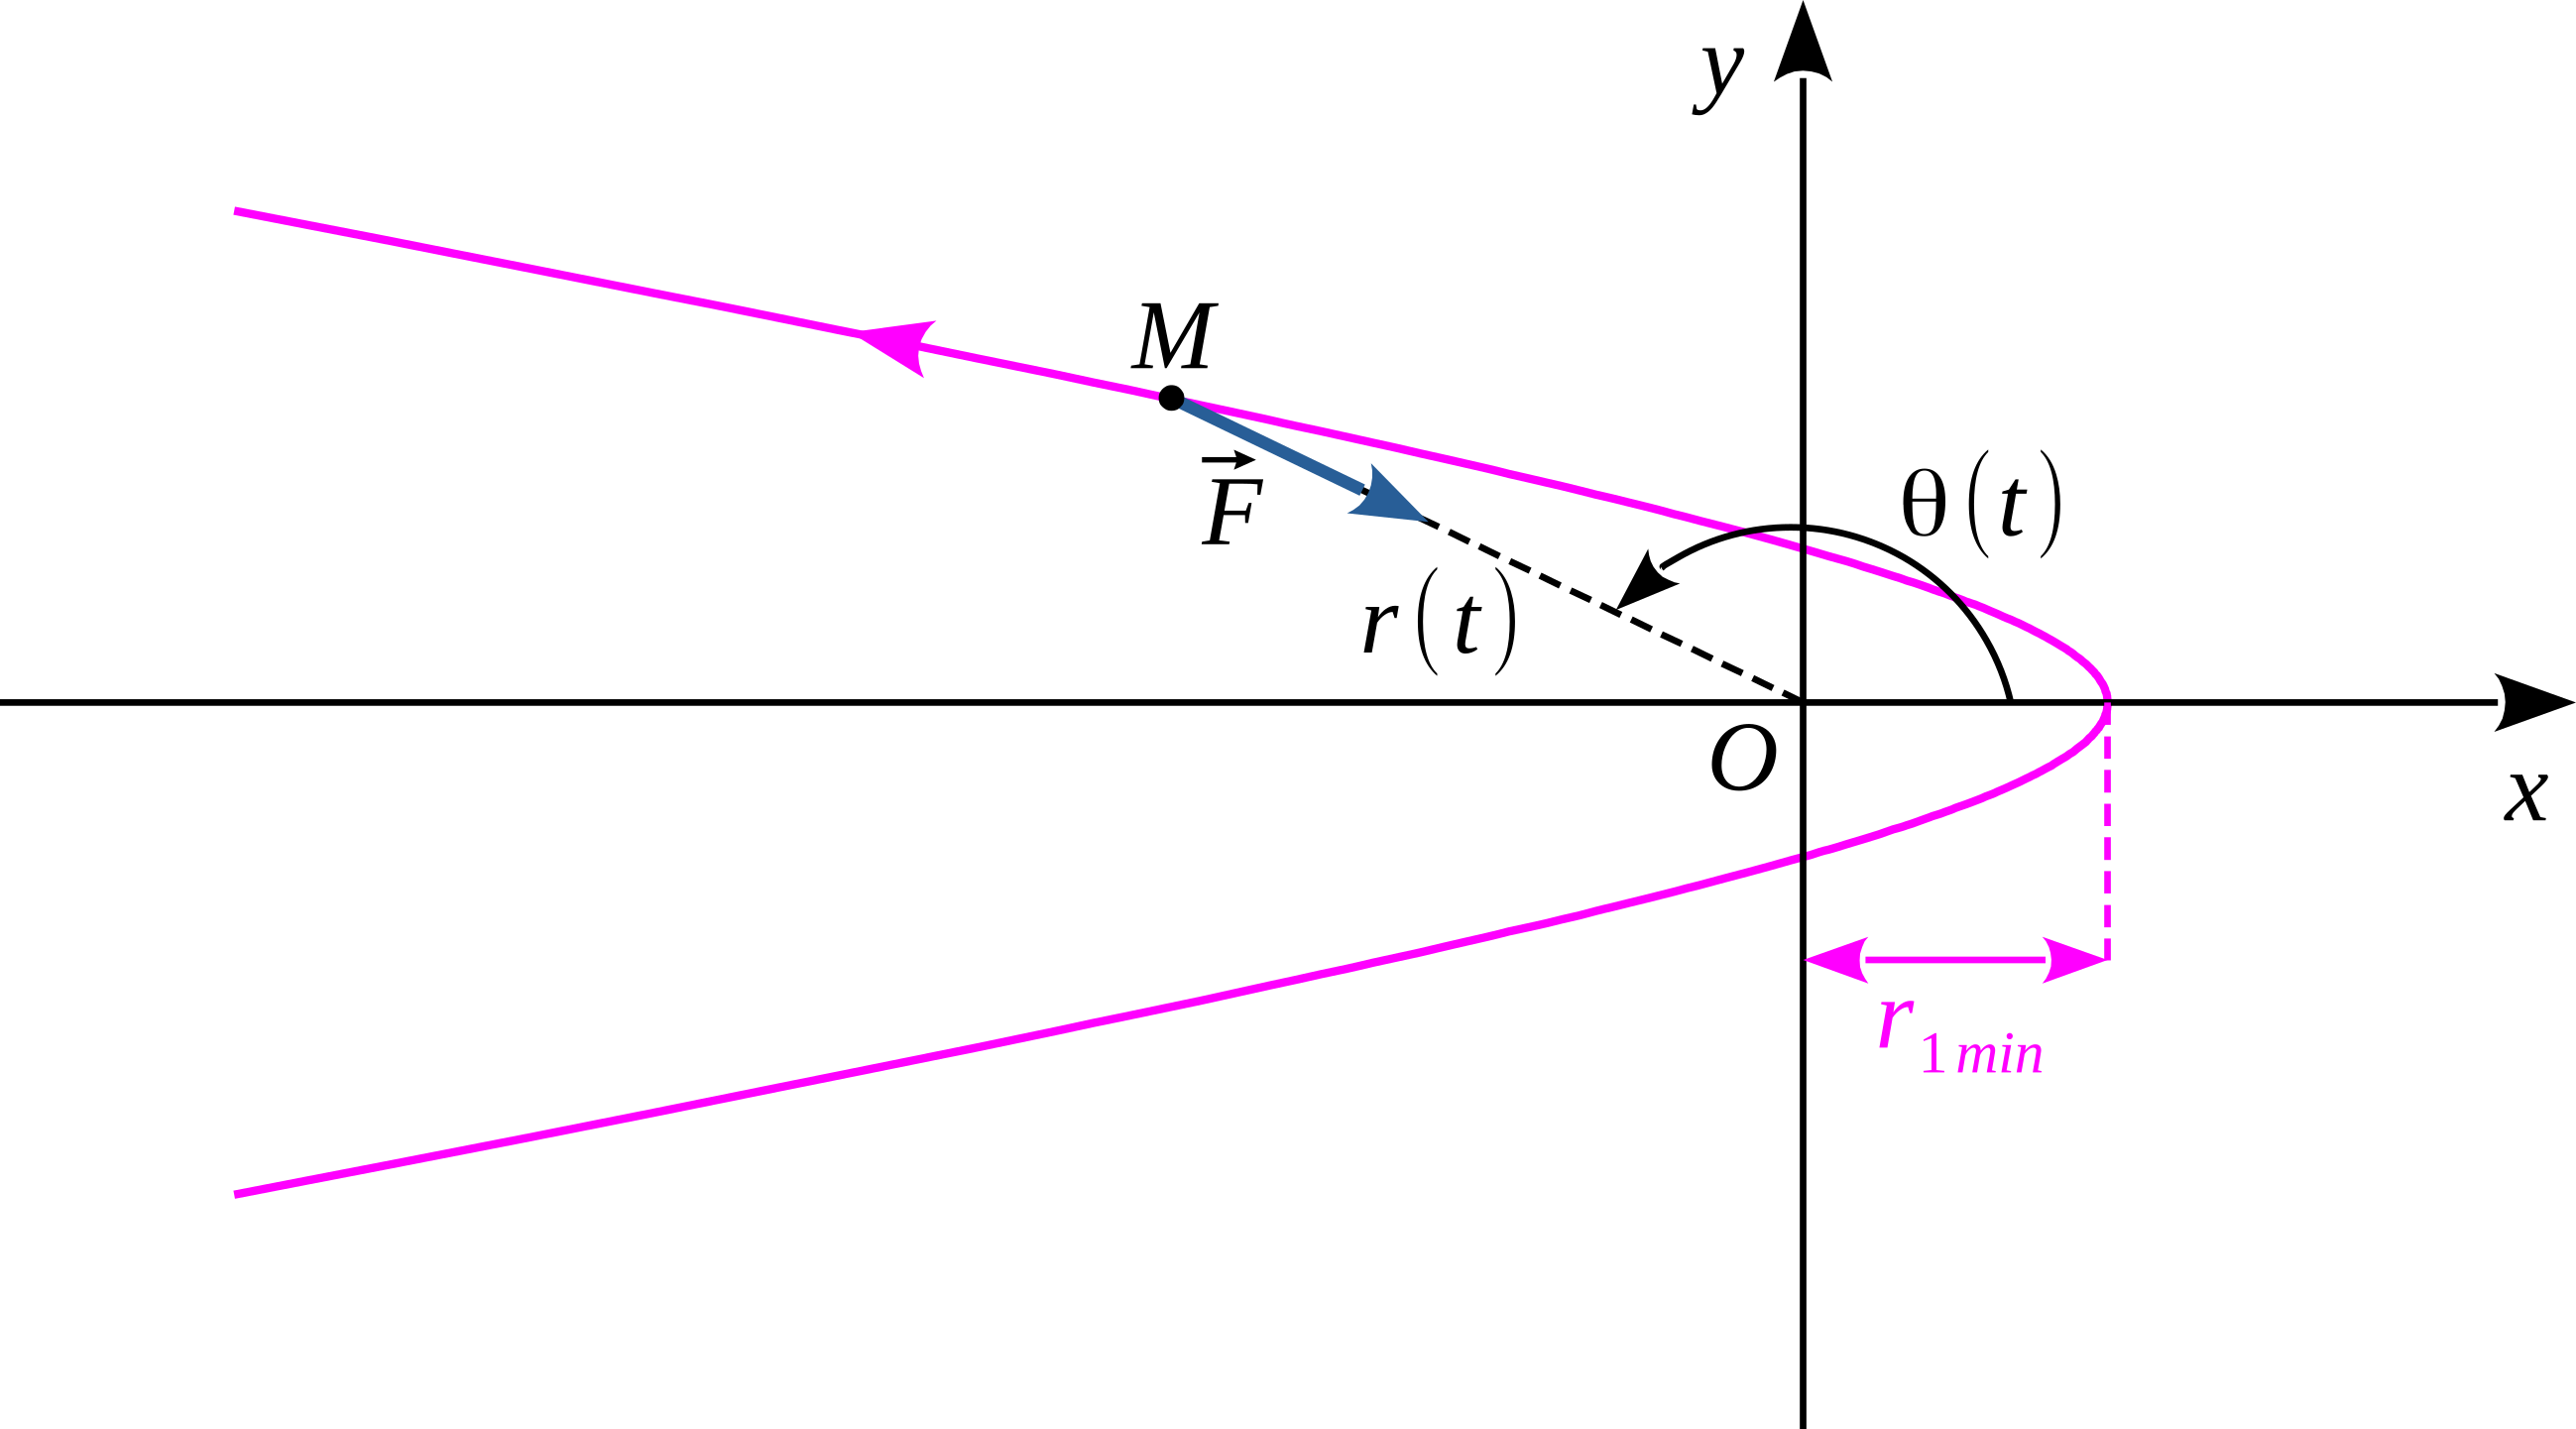
\includegraphics[width=\linewidth]{traj_att-color_hyp} &
%         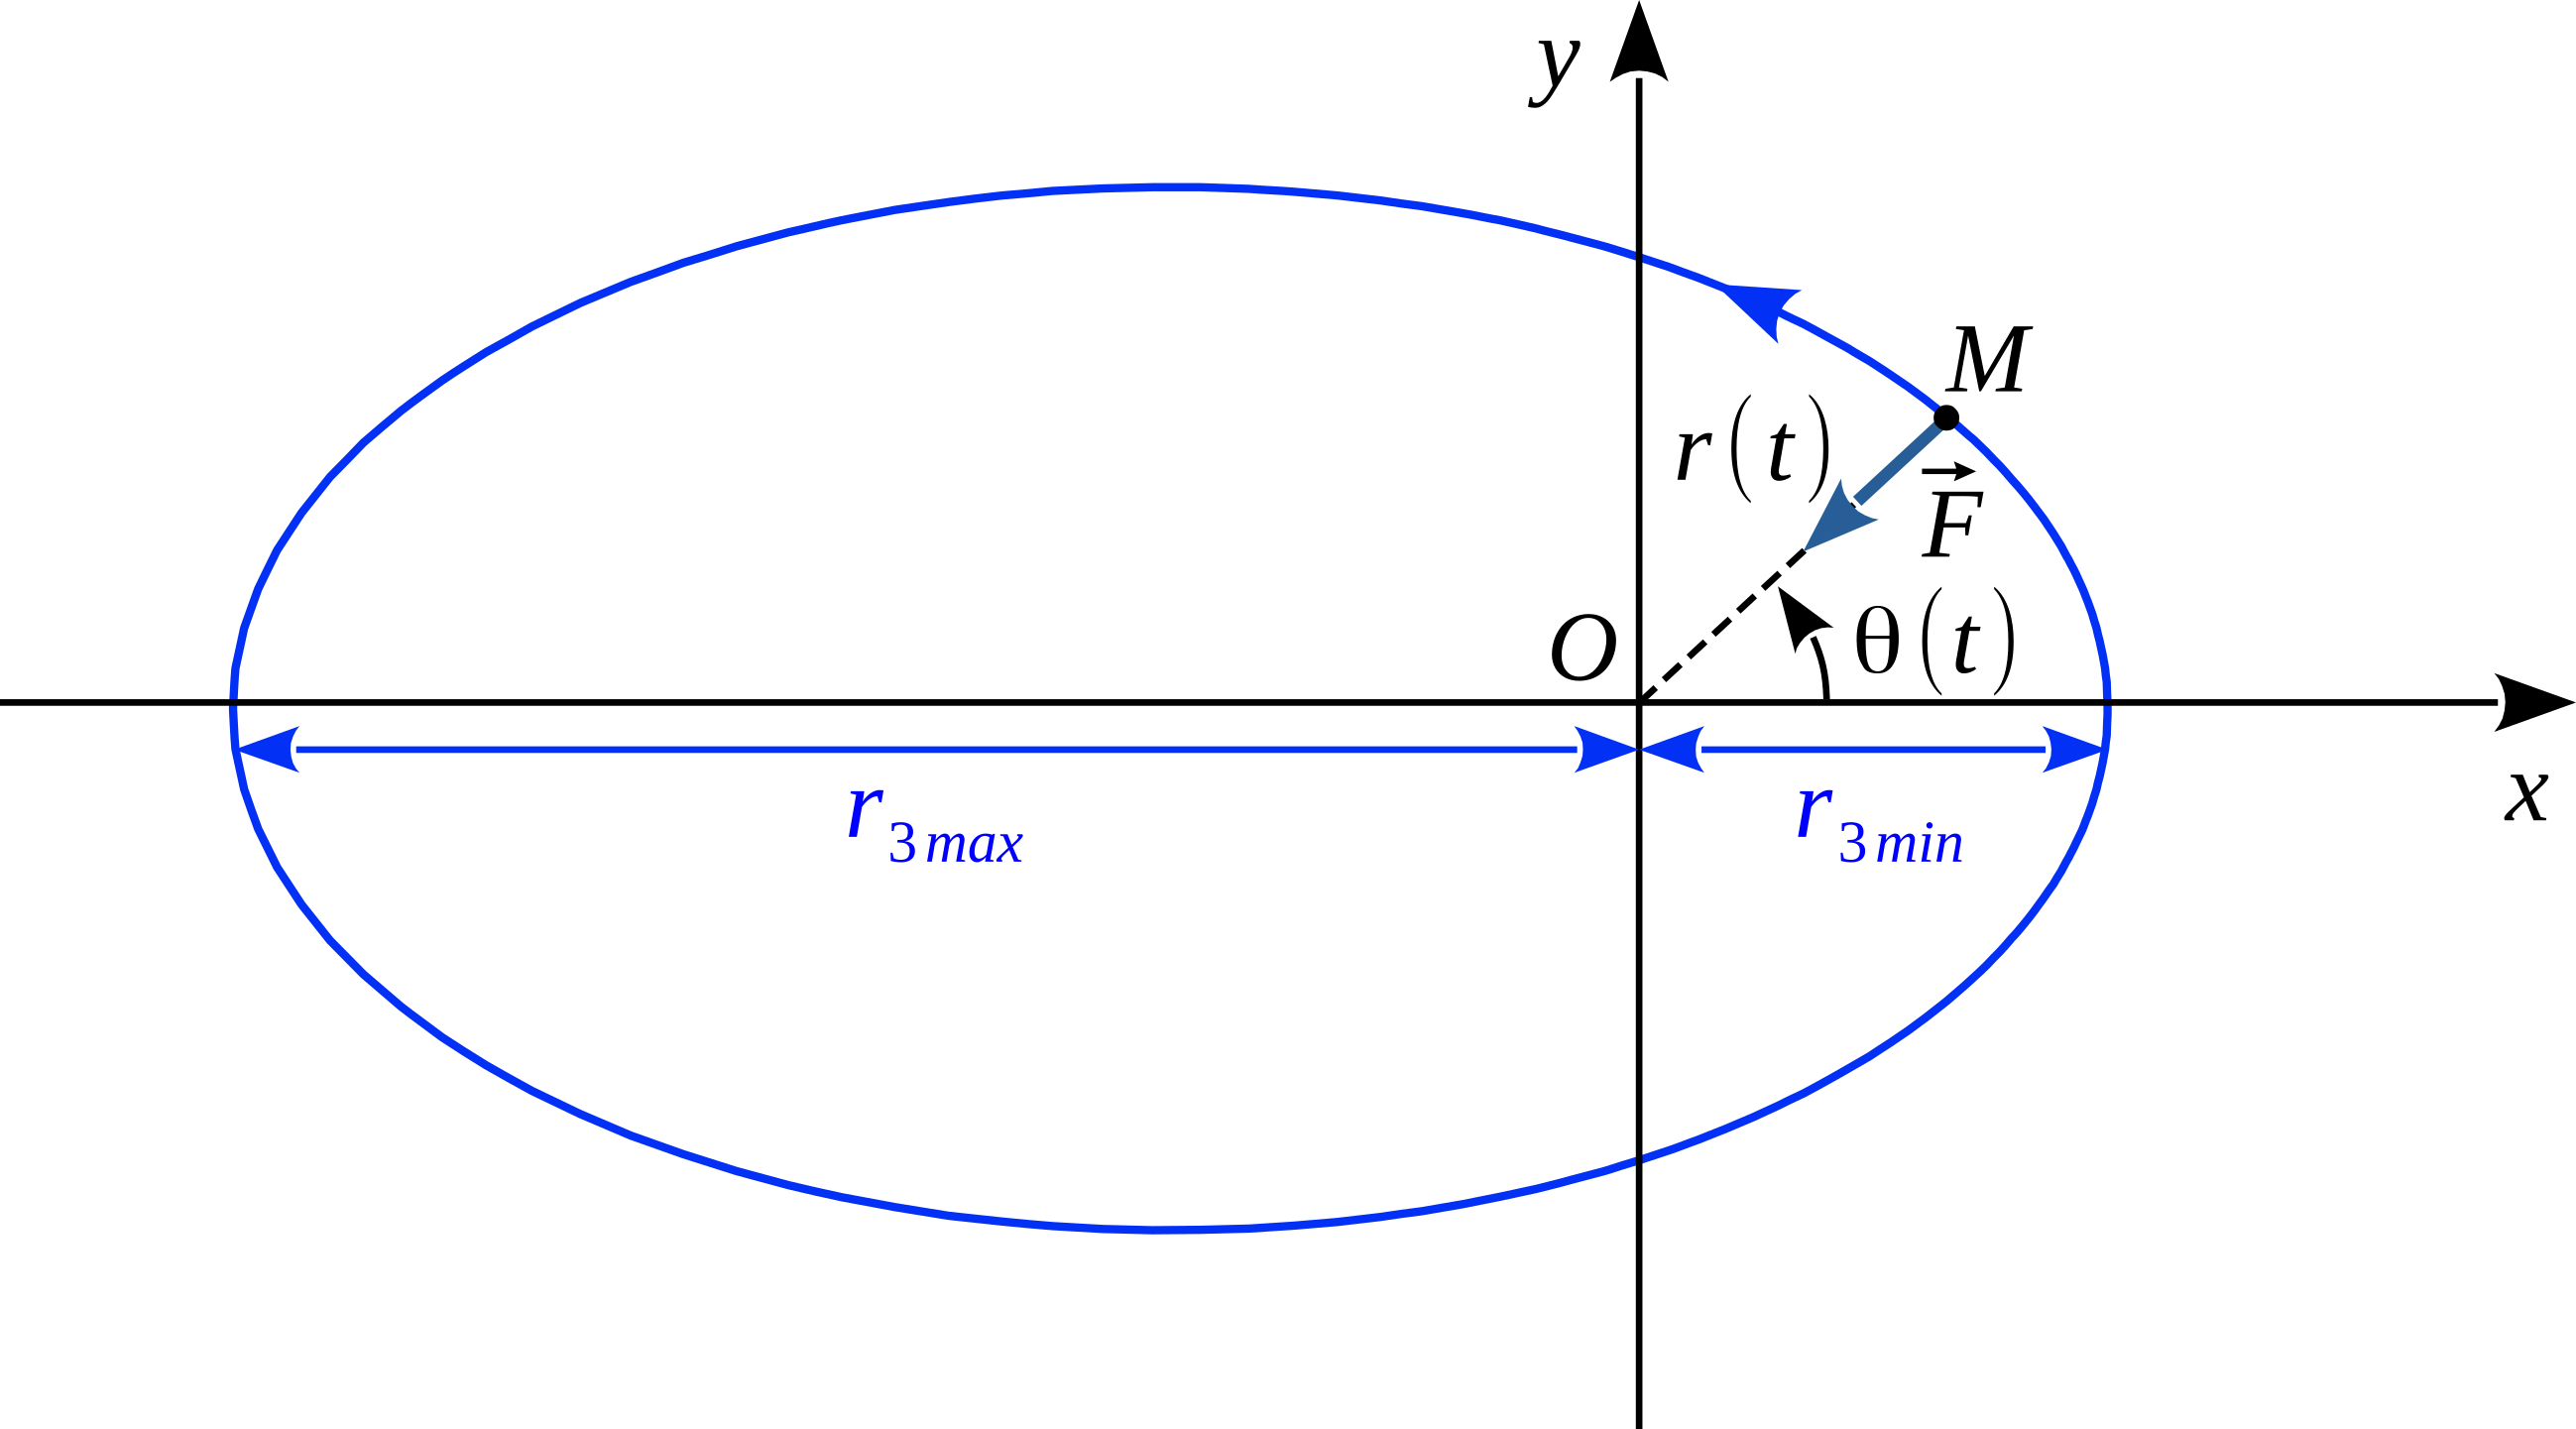
\includegraphics[width=\linewidth]{traj_att-color_ell}
%         \\
%         Trajectoire &
%         \textbf{hyperbolique} &
%         \textbf{elliptique}
%         \\\midrule
%         Valeur de $\Ec_m$ &
%         $\Ec_m = 0$ &
%         $0 < \Ec_m < \infty$
%         \\
%         Graphique &
%         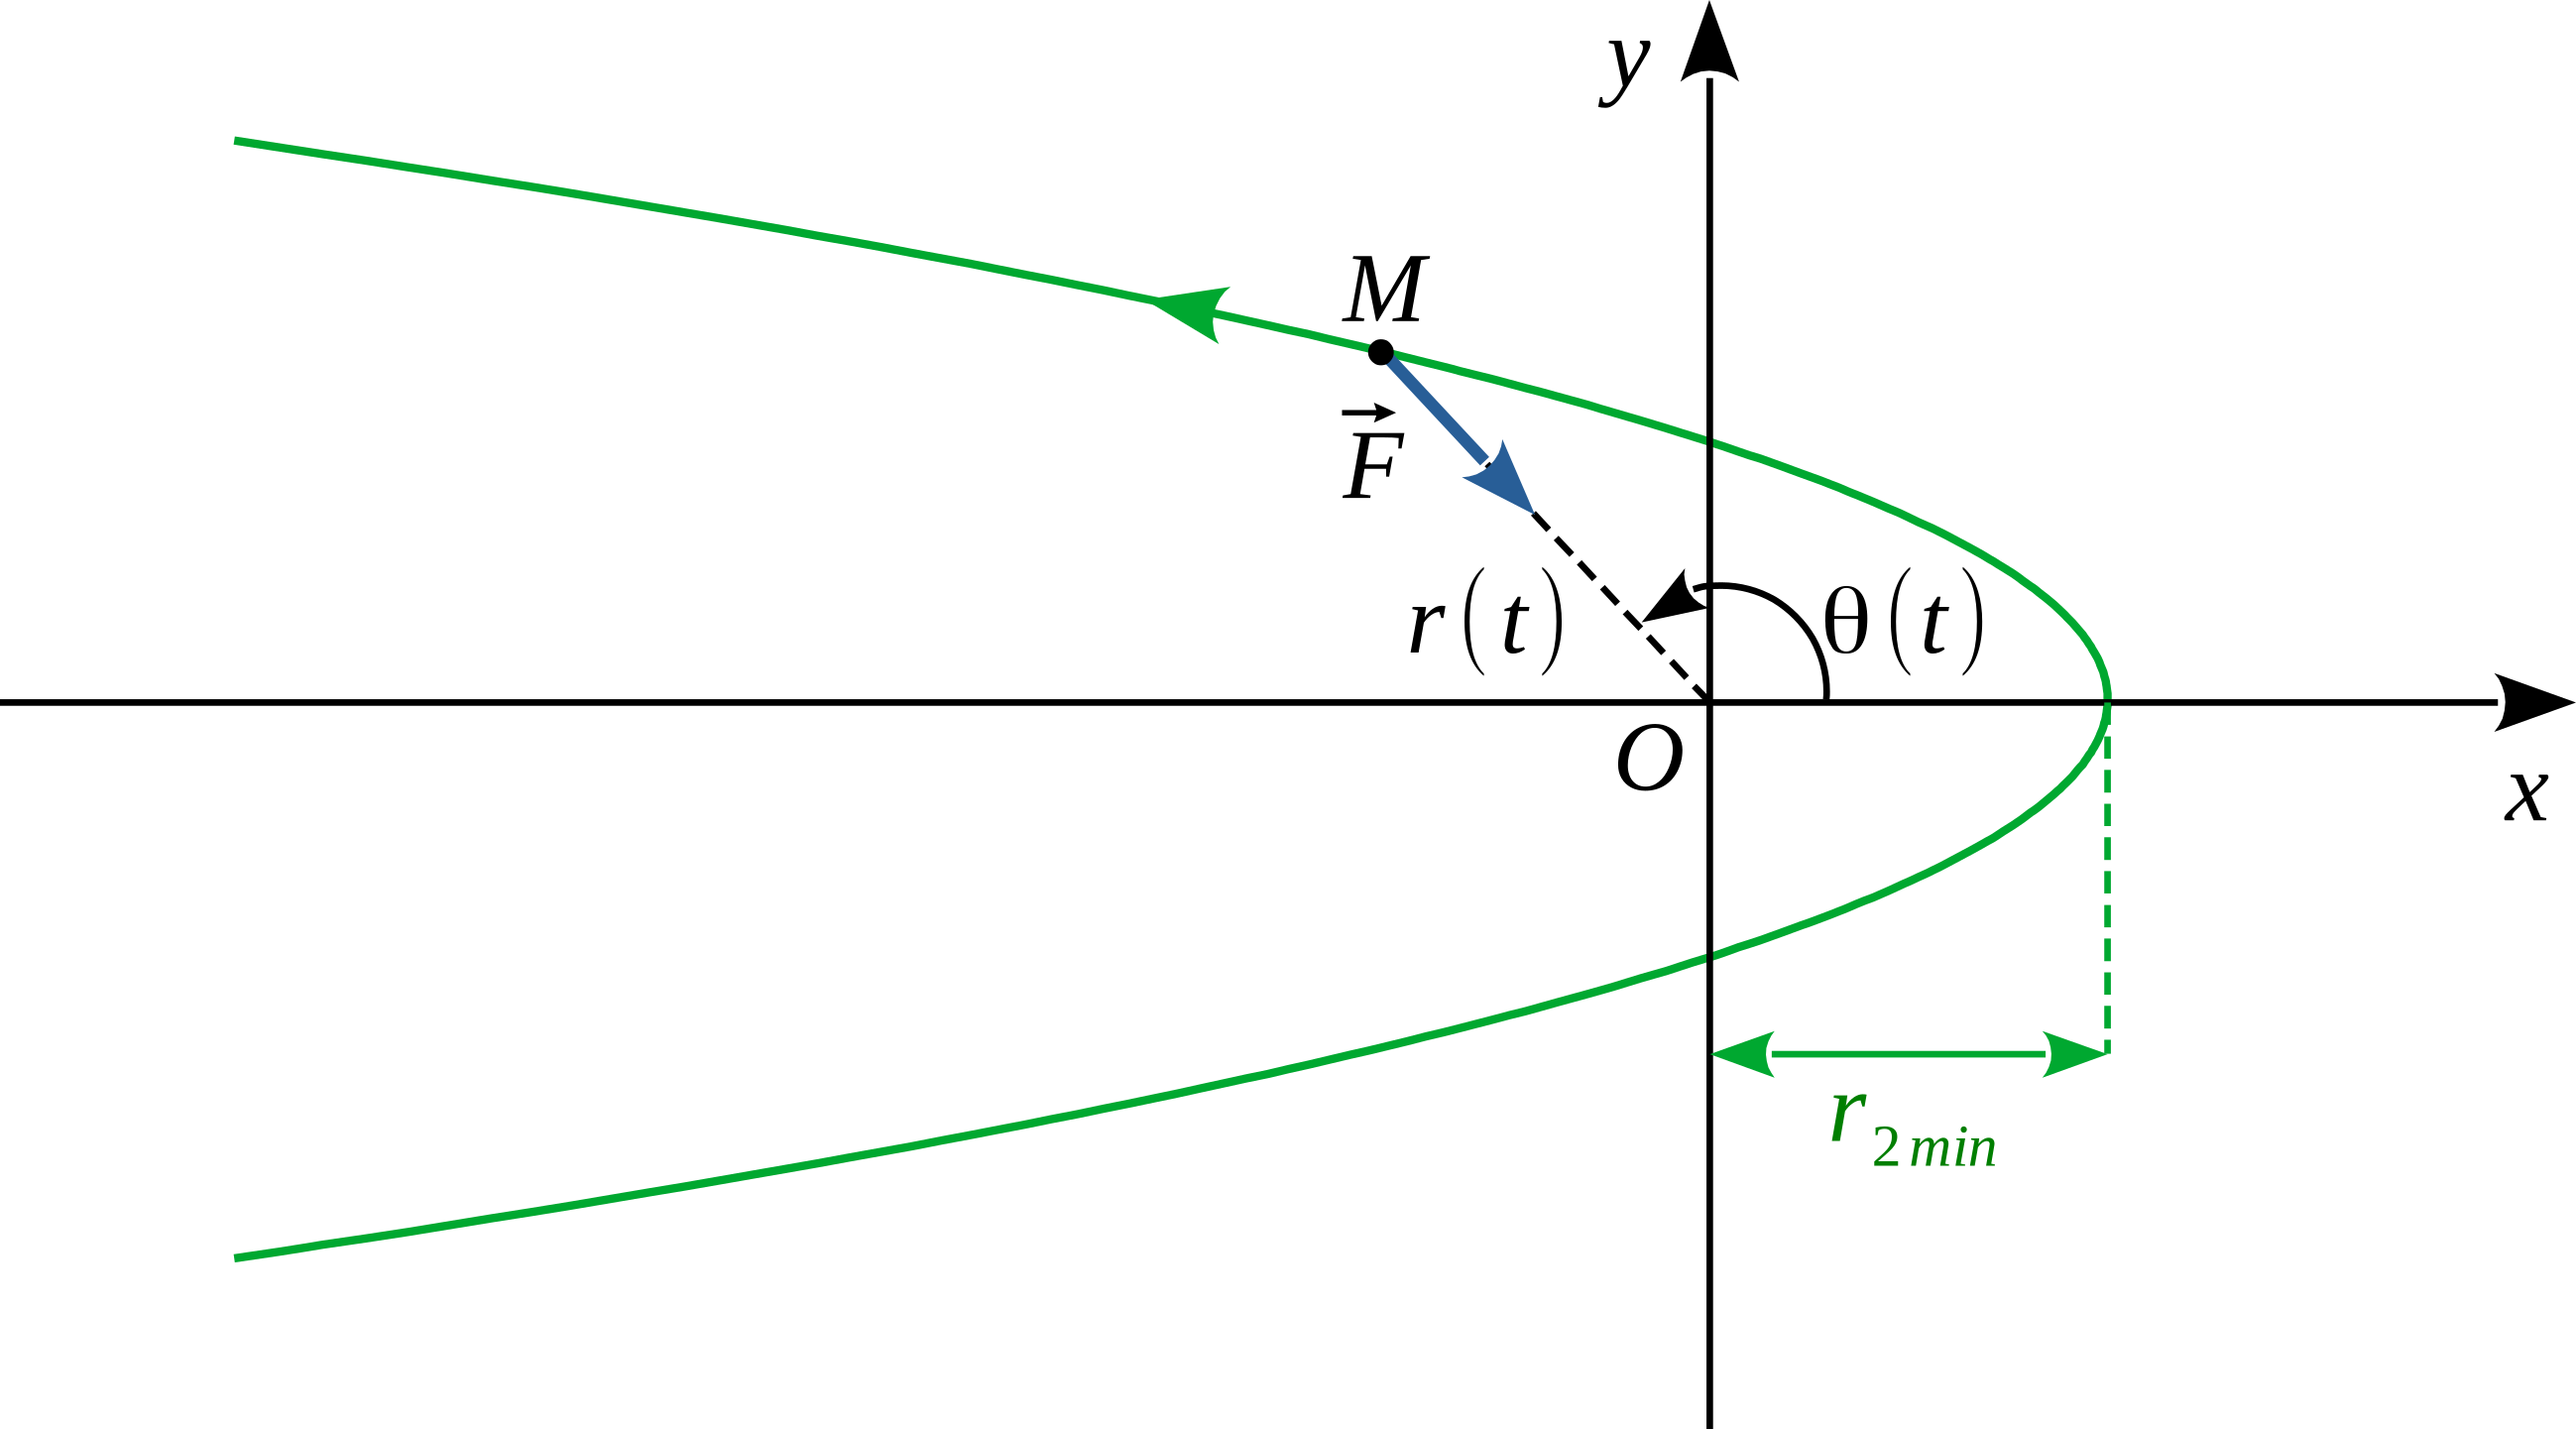
\includegraphics[width=\linewidth]{traj_att-color_par} &
%         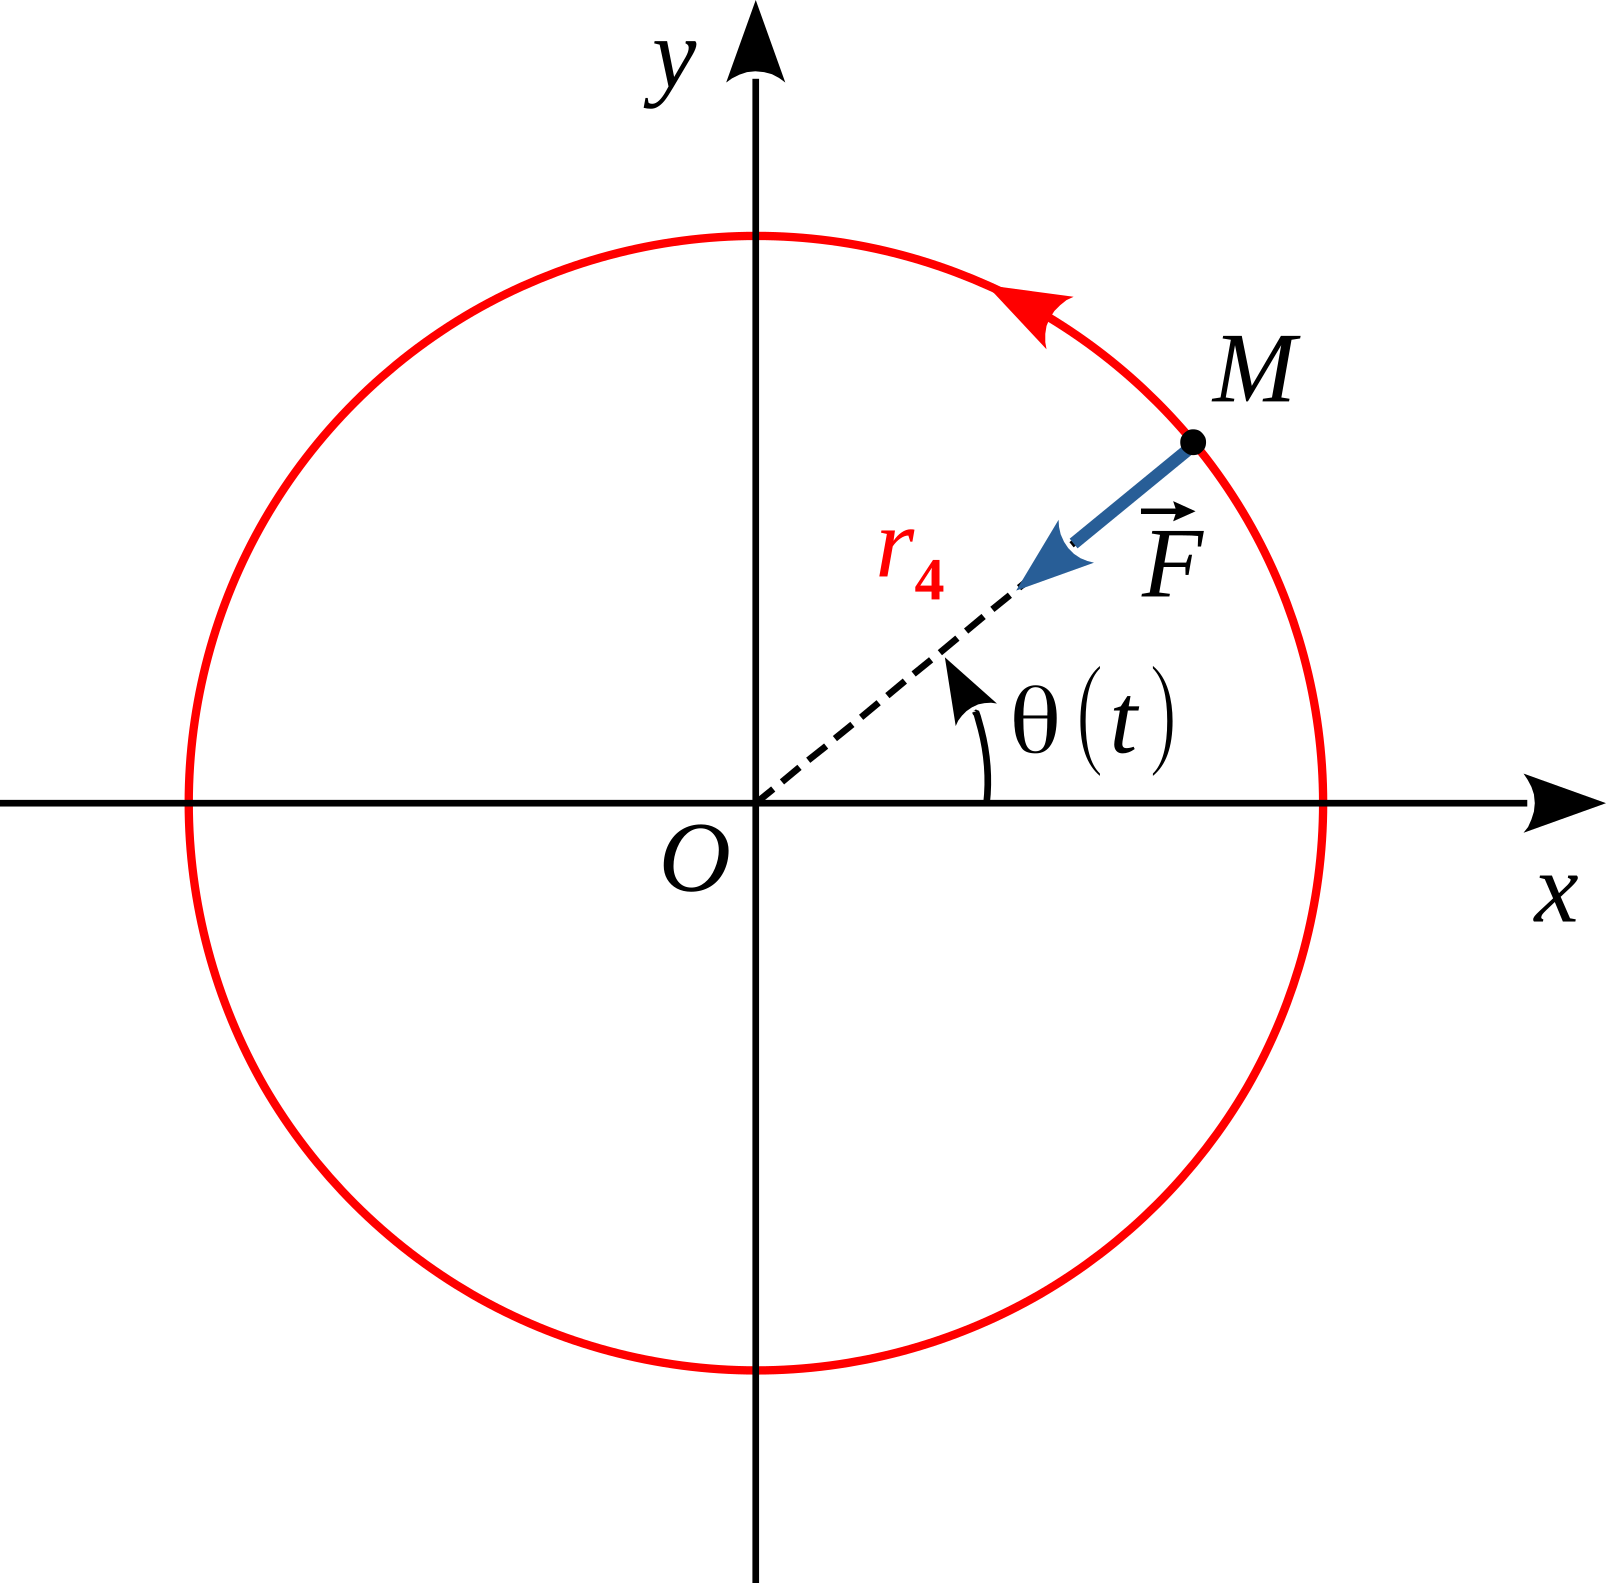
\includegraphics[scale=.7]{traj_att-color_cer}
%         \\
%         Trajectoire &
%         \textbf{parabolique} &
%         \textbf{circulaire}
%         \\\bottomrule
%     \end{tabularx}
% \end{table}

\begin{table}[h]
	\begin{tabularx}{\linewidth}{llYY}
		\toprule
		\multicolumn{2}{c}{Type de mouvement }
		                   &
		\multicolumn{2}{c}{Caractéristiques}
		\\\midrule
		\textbf{Diffusion} & $0 \leq \Ec_m$ &
		$0 < \Ec_m < \infty$
		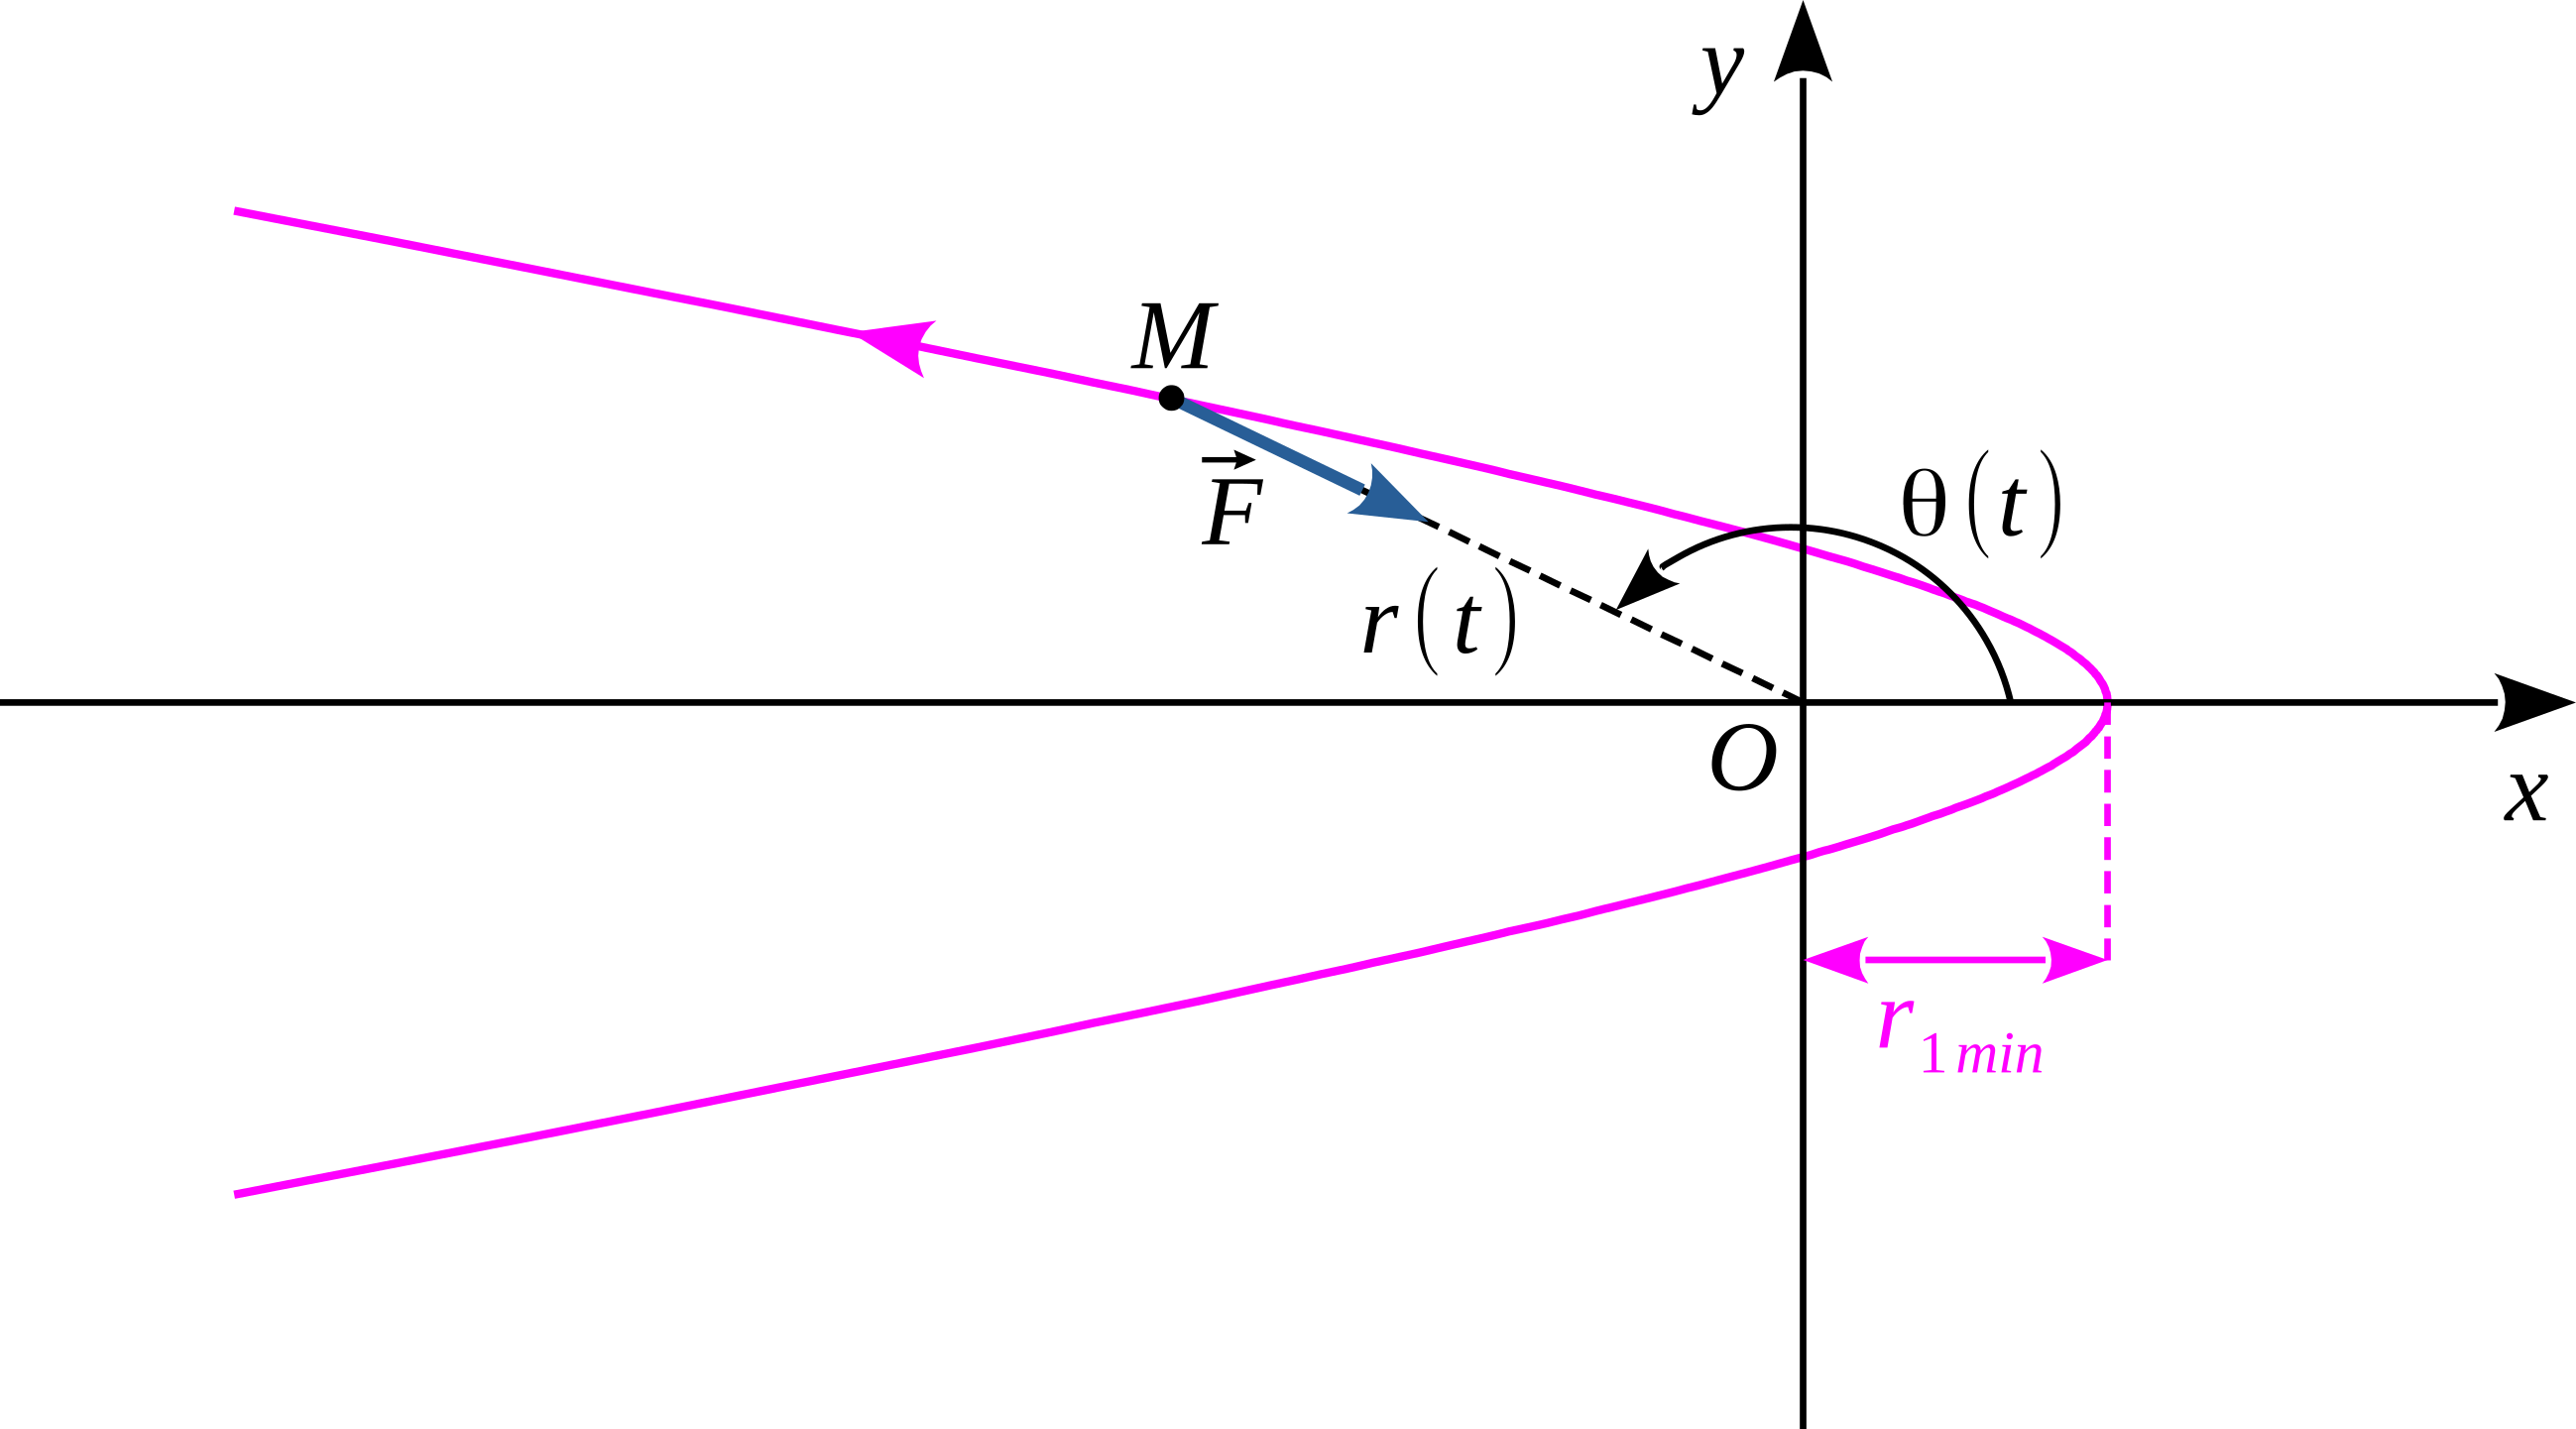
\includegraphics[width=\linewidth]{traj_att-color_hyp}
		Trajectoire \textbf{hyperbolique}
		                   &
		$\Ec_m = 0$
		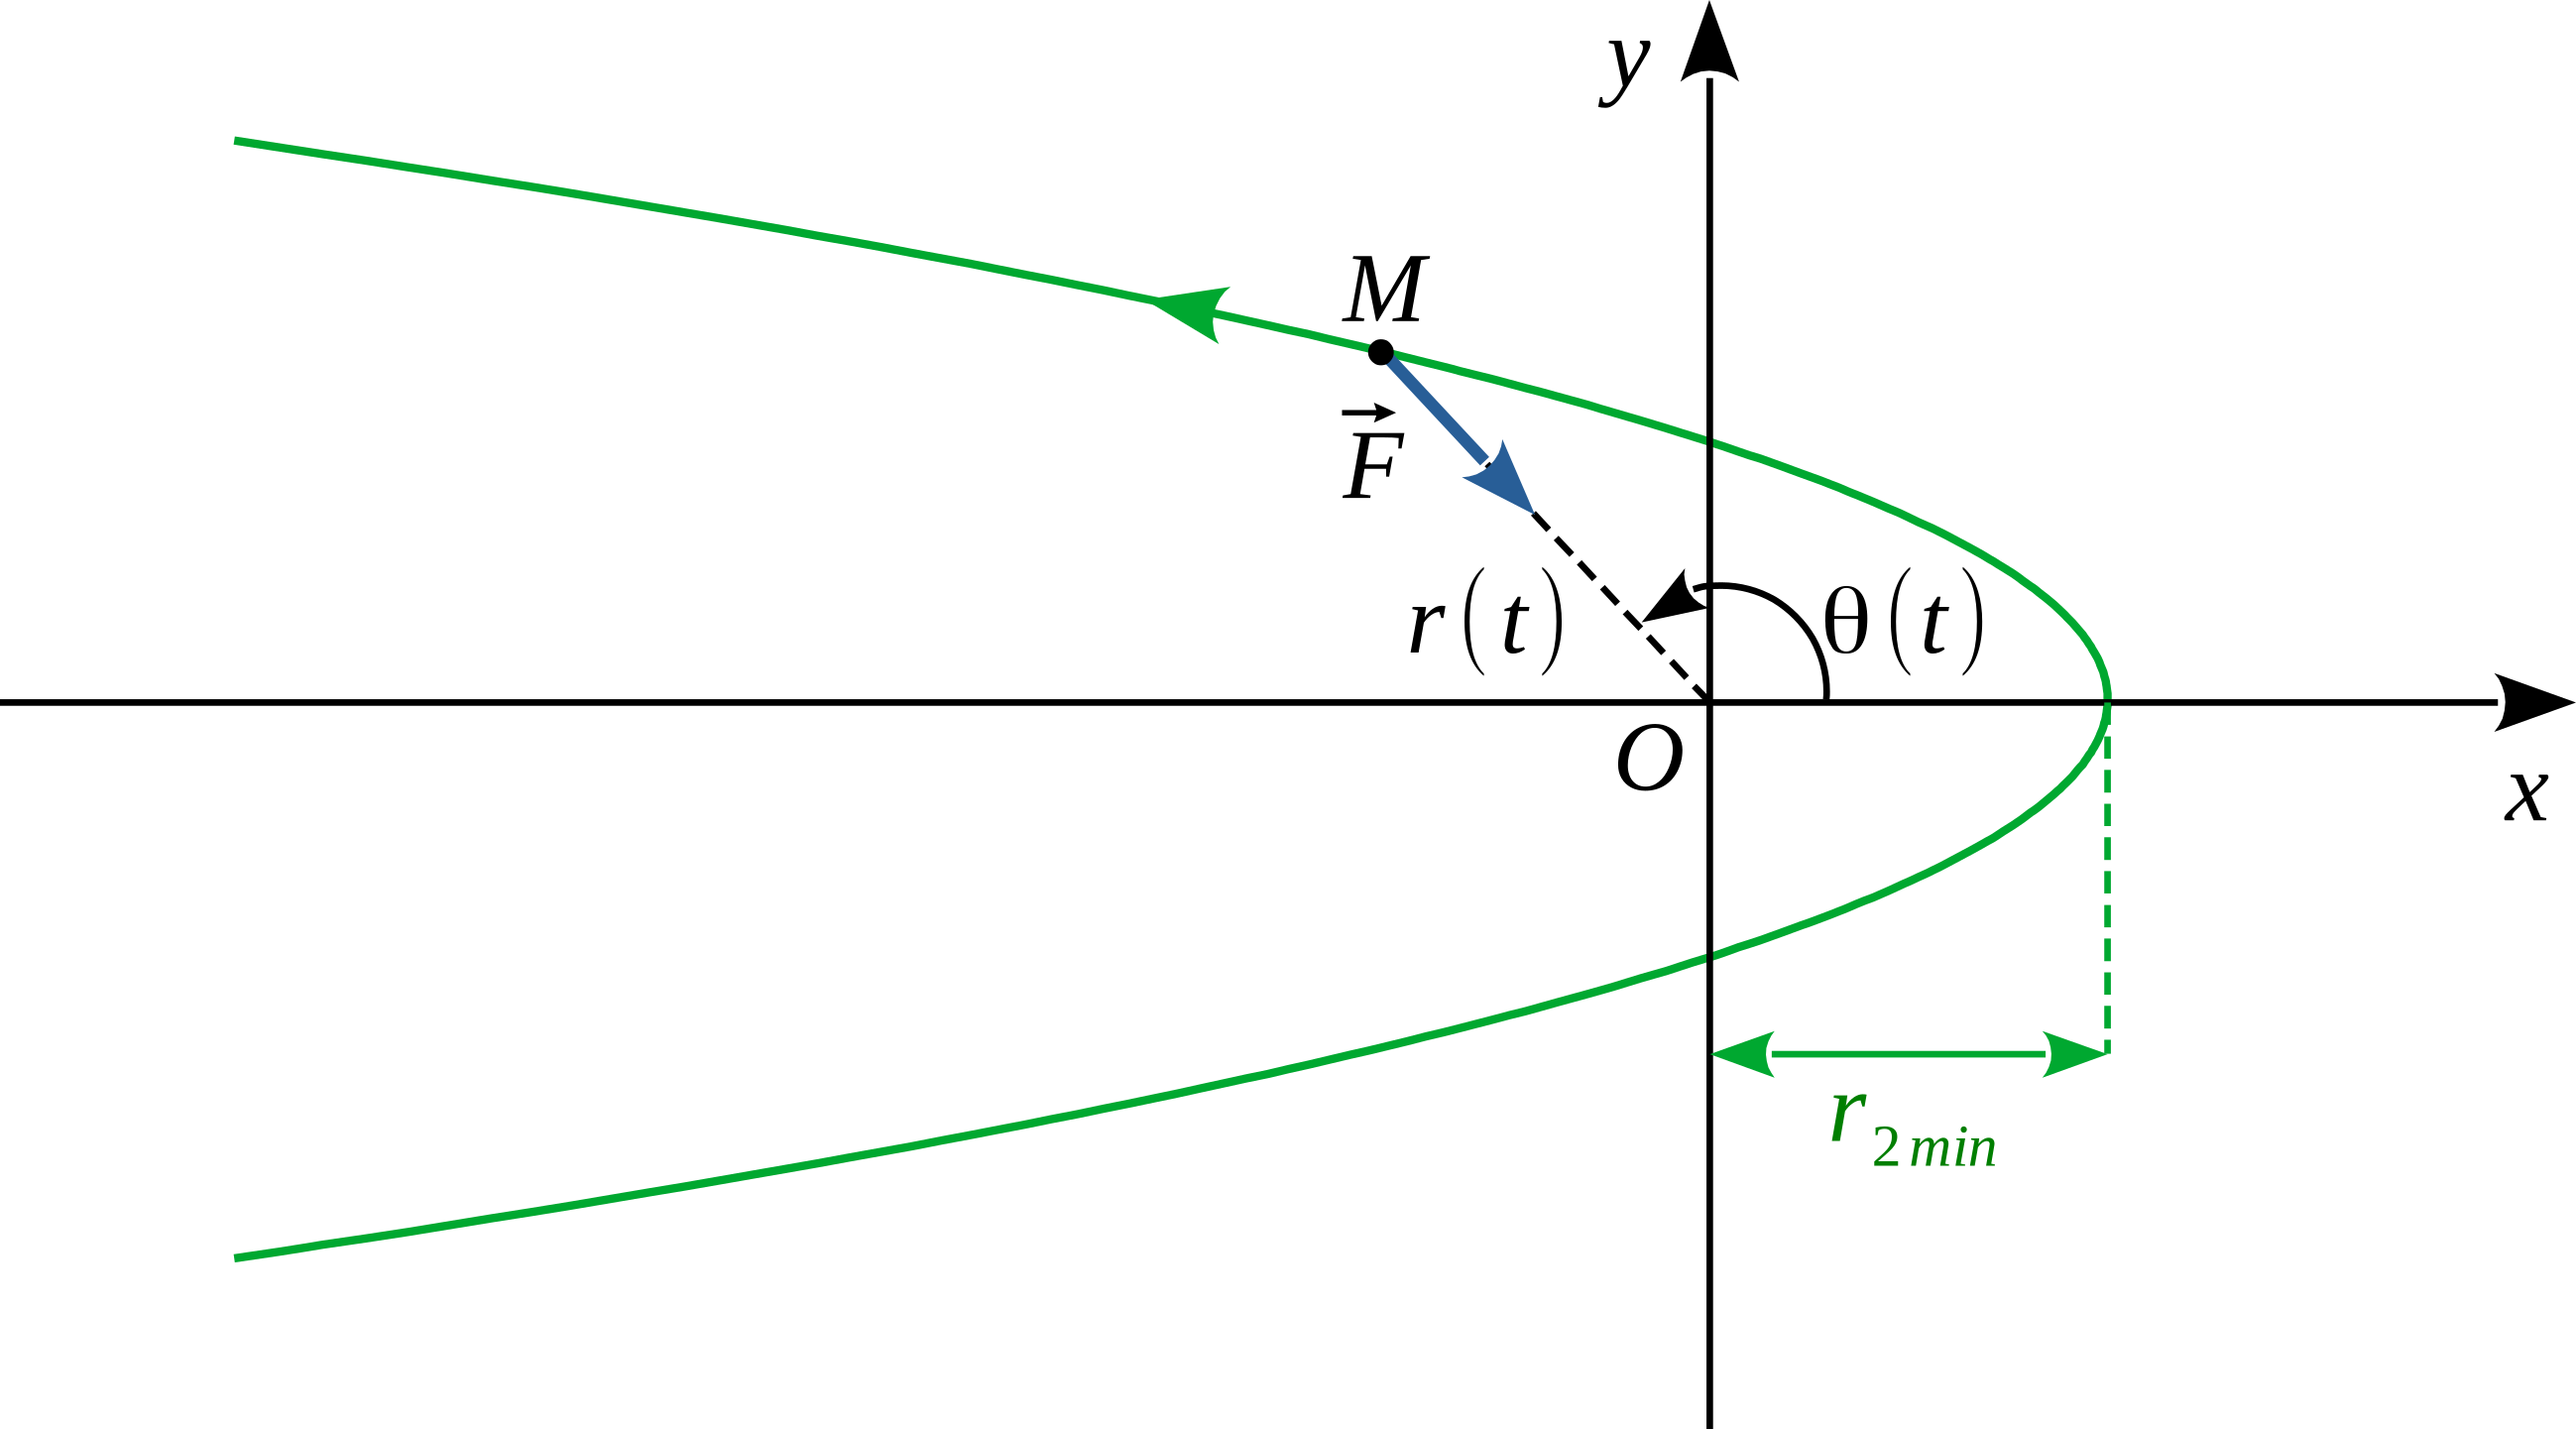
\includegraphics[width=\linewidth]{traj_att-color_par}
		Trajectoire \textbf{parabolique}
		\\\midrule
		\textbf{Lié}       & $\Ec_m < 0$    &
		$-\Ec_0 < \Ec_m < 0$
		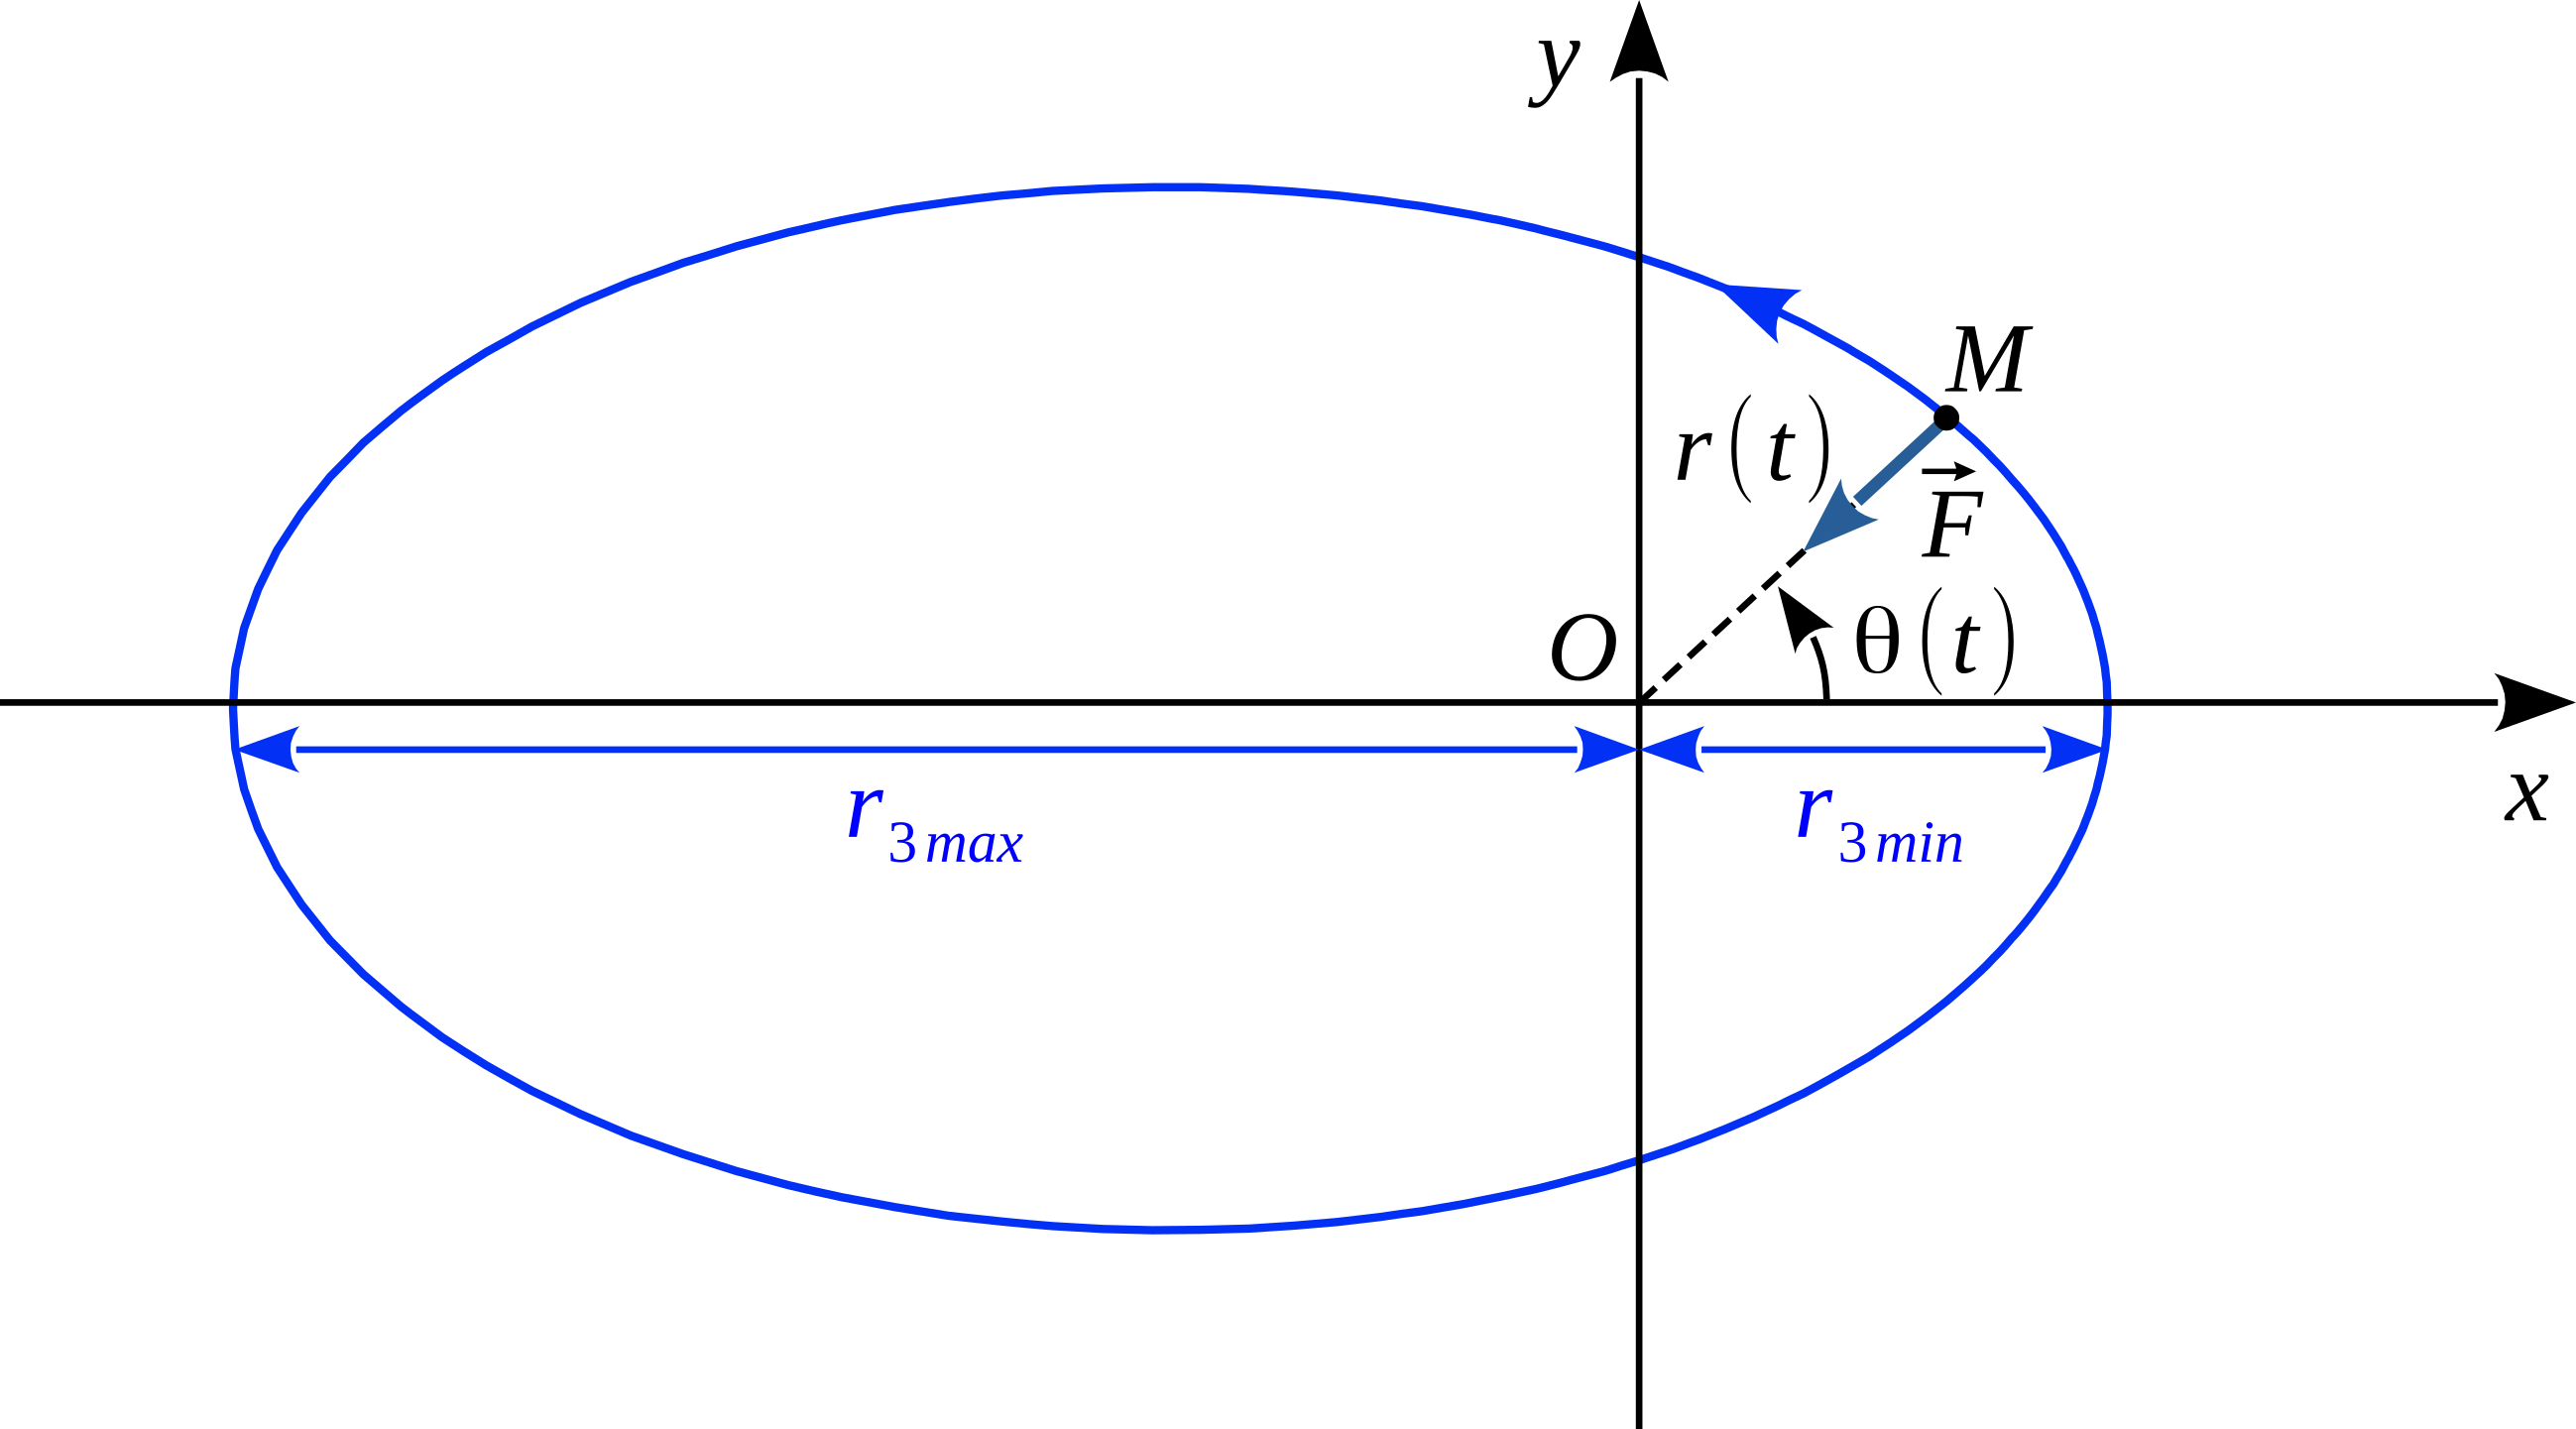
\includegraphics[width=\linewidth]{traj_att-color_ell}
		Trajectoire \textbf{elliptique}
		                   &
		$\Ec_m = -\Ec_0$
		\smallbreak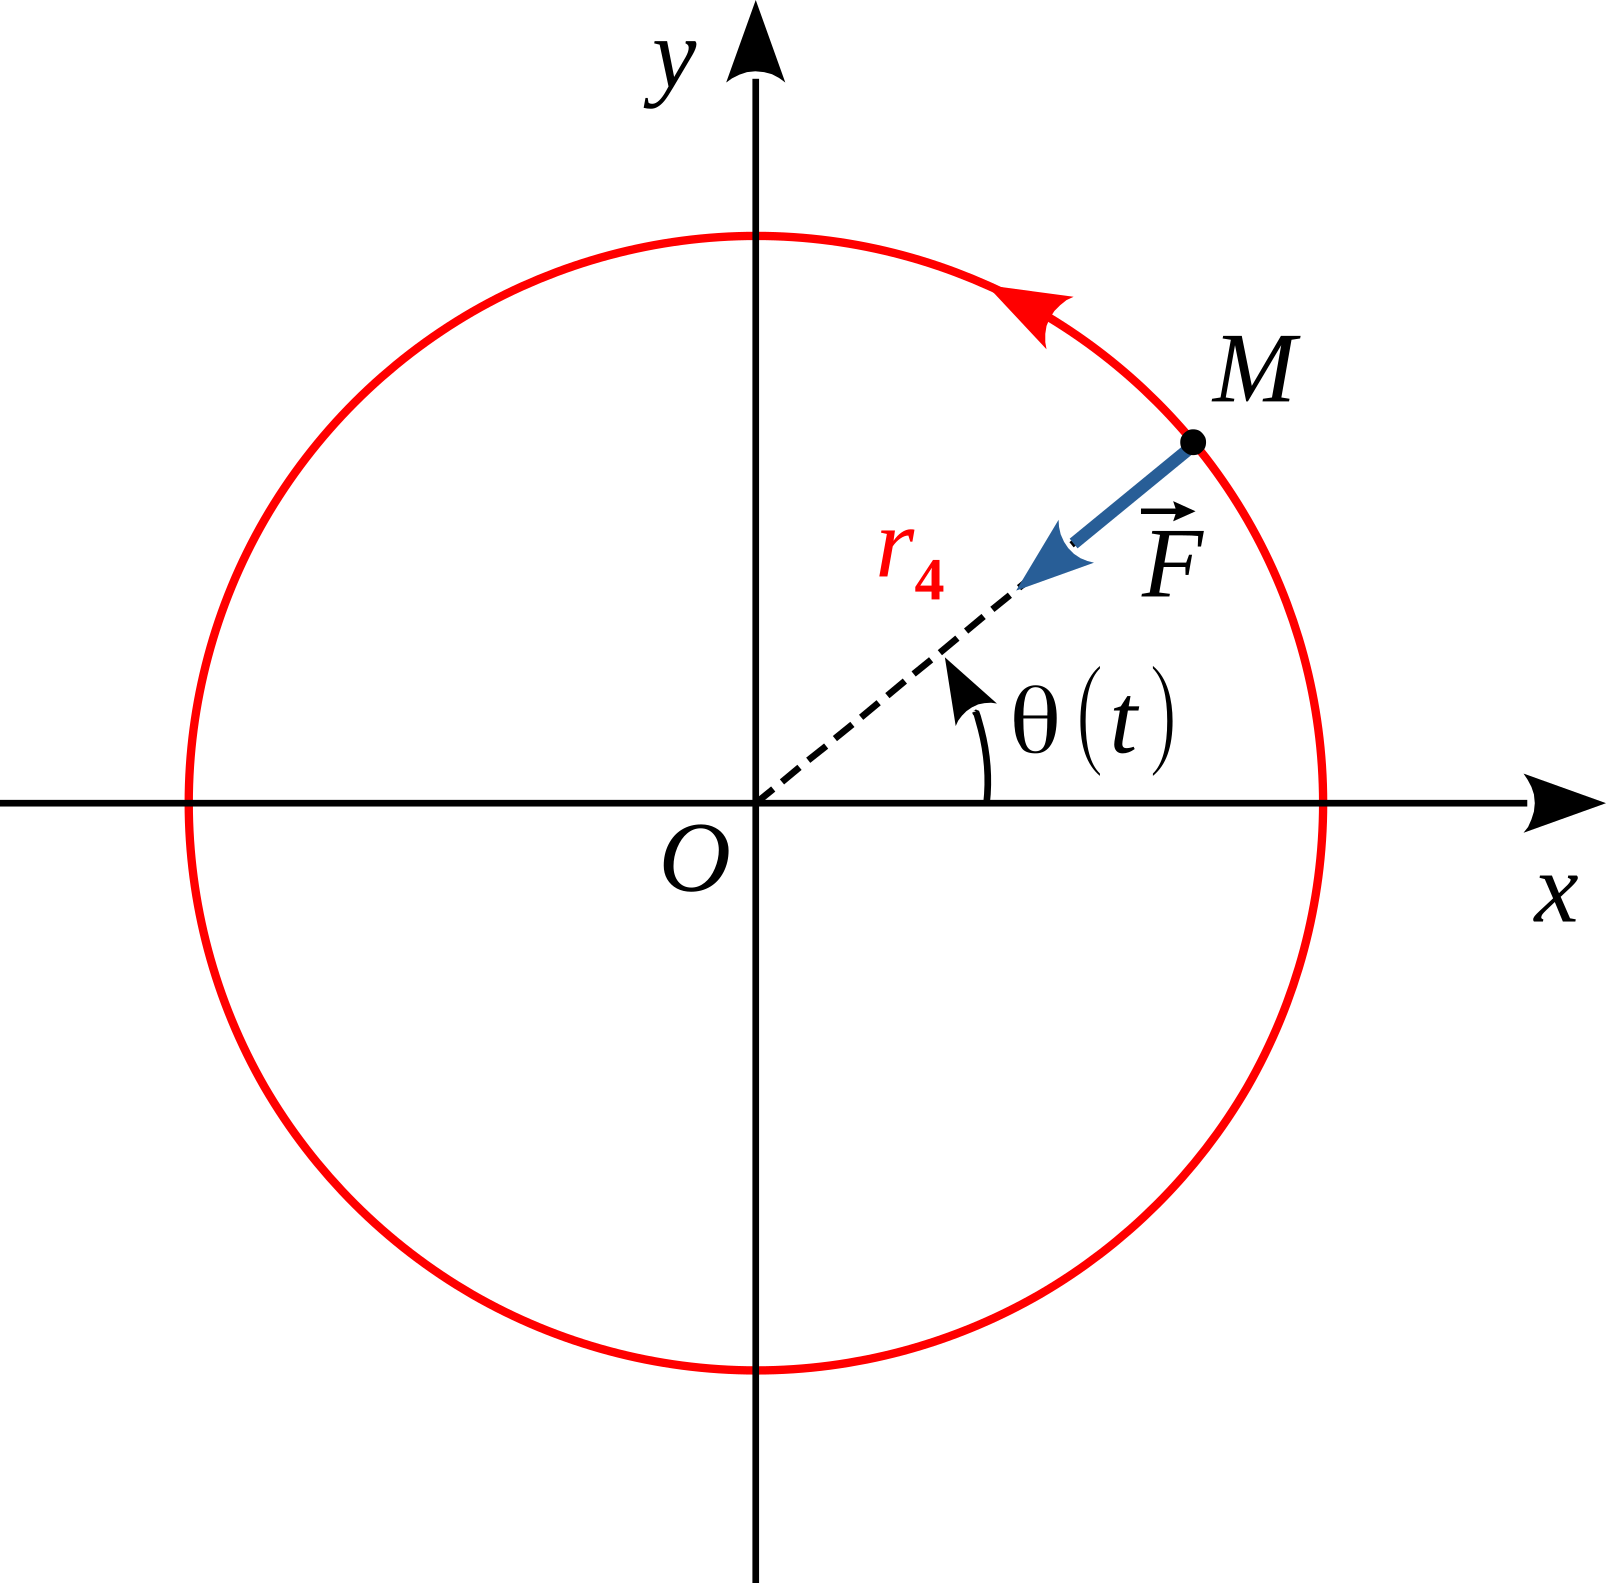
\includegraphics[scale=.6]{traj_att-color_cer}\smallbreak
		Trajectoire \textbf{circulaire}
		\\\bottomrule
	\end{tabularx}
\end{table}

\begin{tcb*}[sidebyside, righthand ratio=.4](exem)<lftt>{État lié, état de diffusion}
	\begin{itemize}
		\item Les planètes du système solaire restent confinées près du Soleil, ce
		      sont donc des états liés.
		\item Un état de diffusion correspond par exemple au cas d'un comète
		      arrivant vers le Soleil, atteignant une distance minimale avant de
		      retourner à l'infini.
	\end{itemize}
	\tcblower
	\begin{center}
		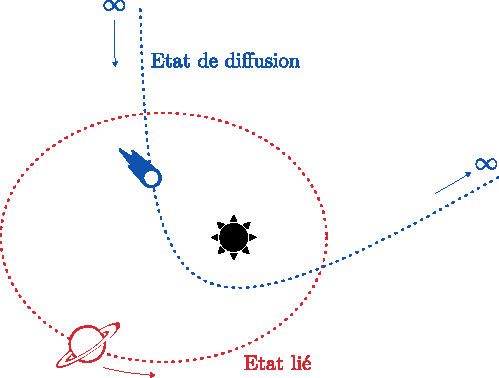
\includegraphics[width=\linewidth]{ep_eff-att_liediff}
	\end{center}
\end{tcb*}

\vspace{-15pt}
\subsection{Cas répulsif}
Ce cas est bien plus simple~: la trajectoire est hyperbolique dans tous les cas.
\smallbreak
\begin{minipage}[c]{0.48\linewidth}
	\begin{center}
		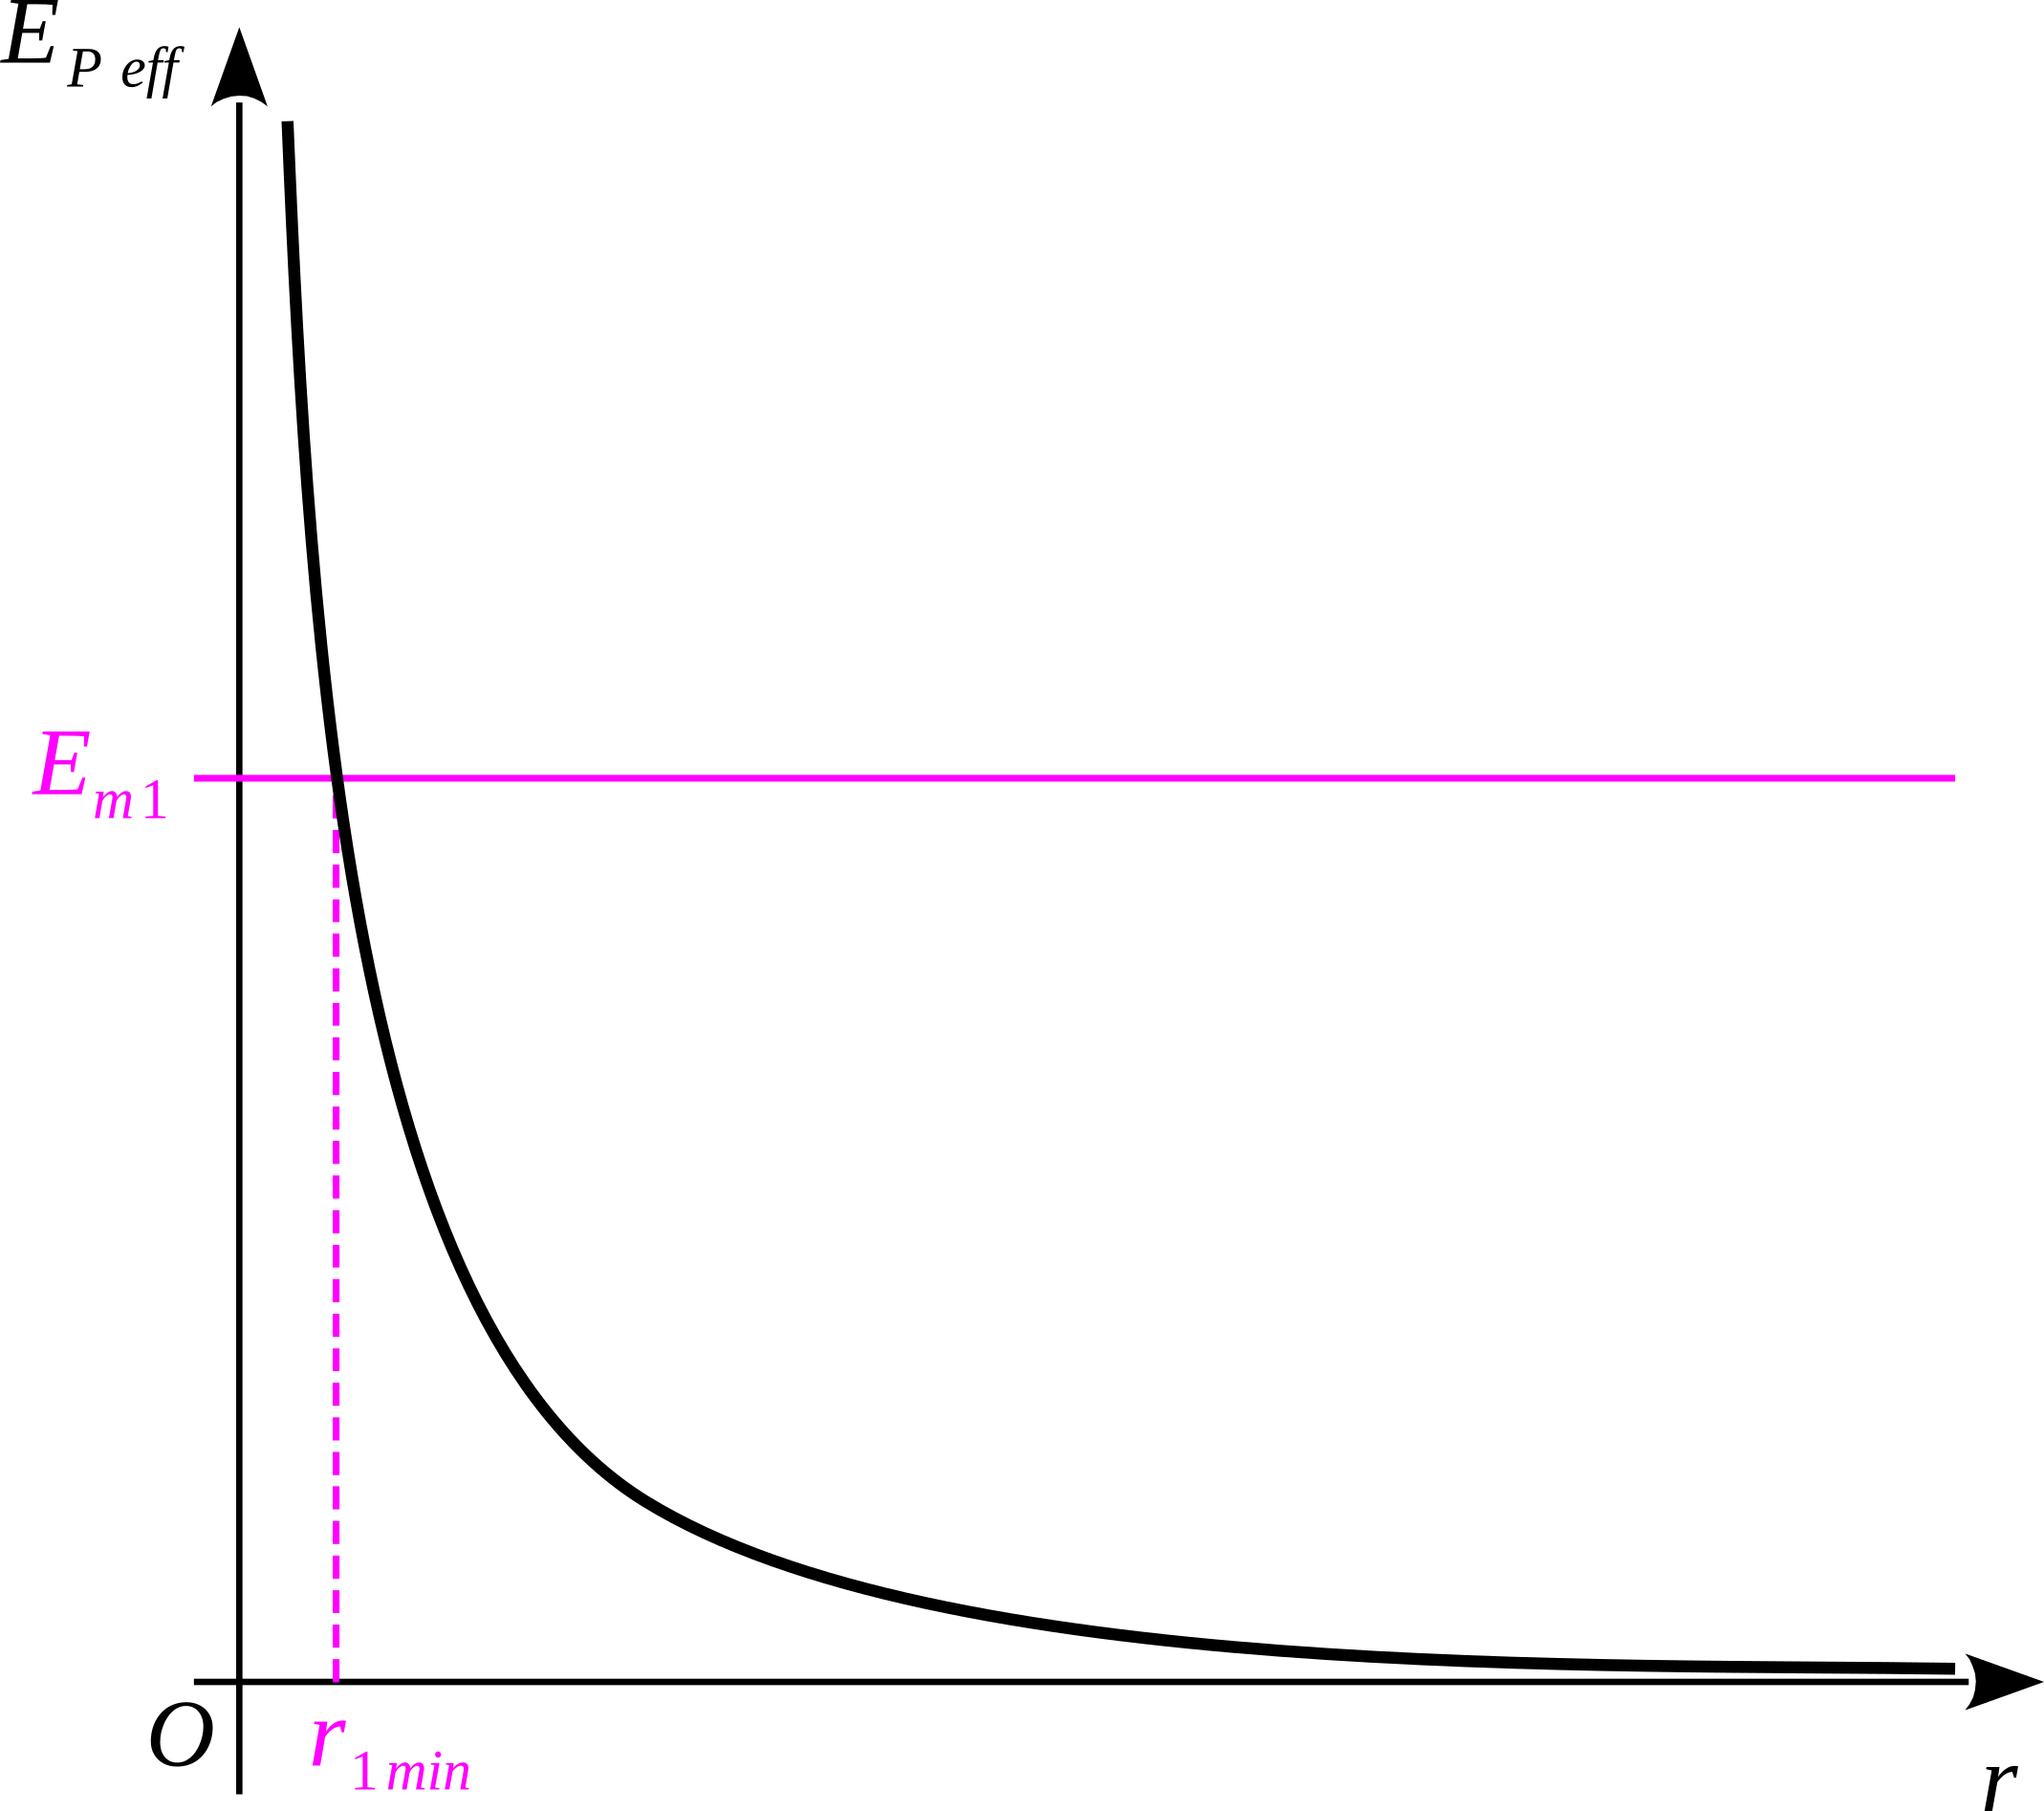
\includegraphics[height=5cm]{ep_eff-rep_color}
		\captionof{figure}{$\Ec_{p,\rm eff}$ cas répulsifs.}
	\end{center}
\end{minipage}
\hfill
\begin{minipage}[c]{0.48\linewidth}
	\begin{center}
		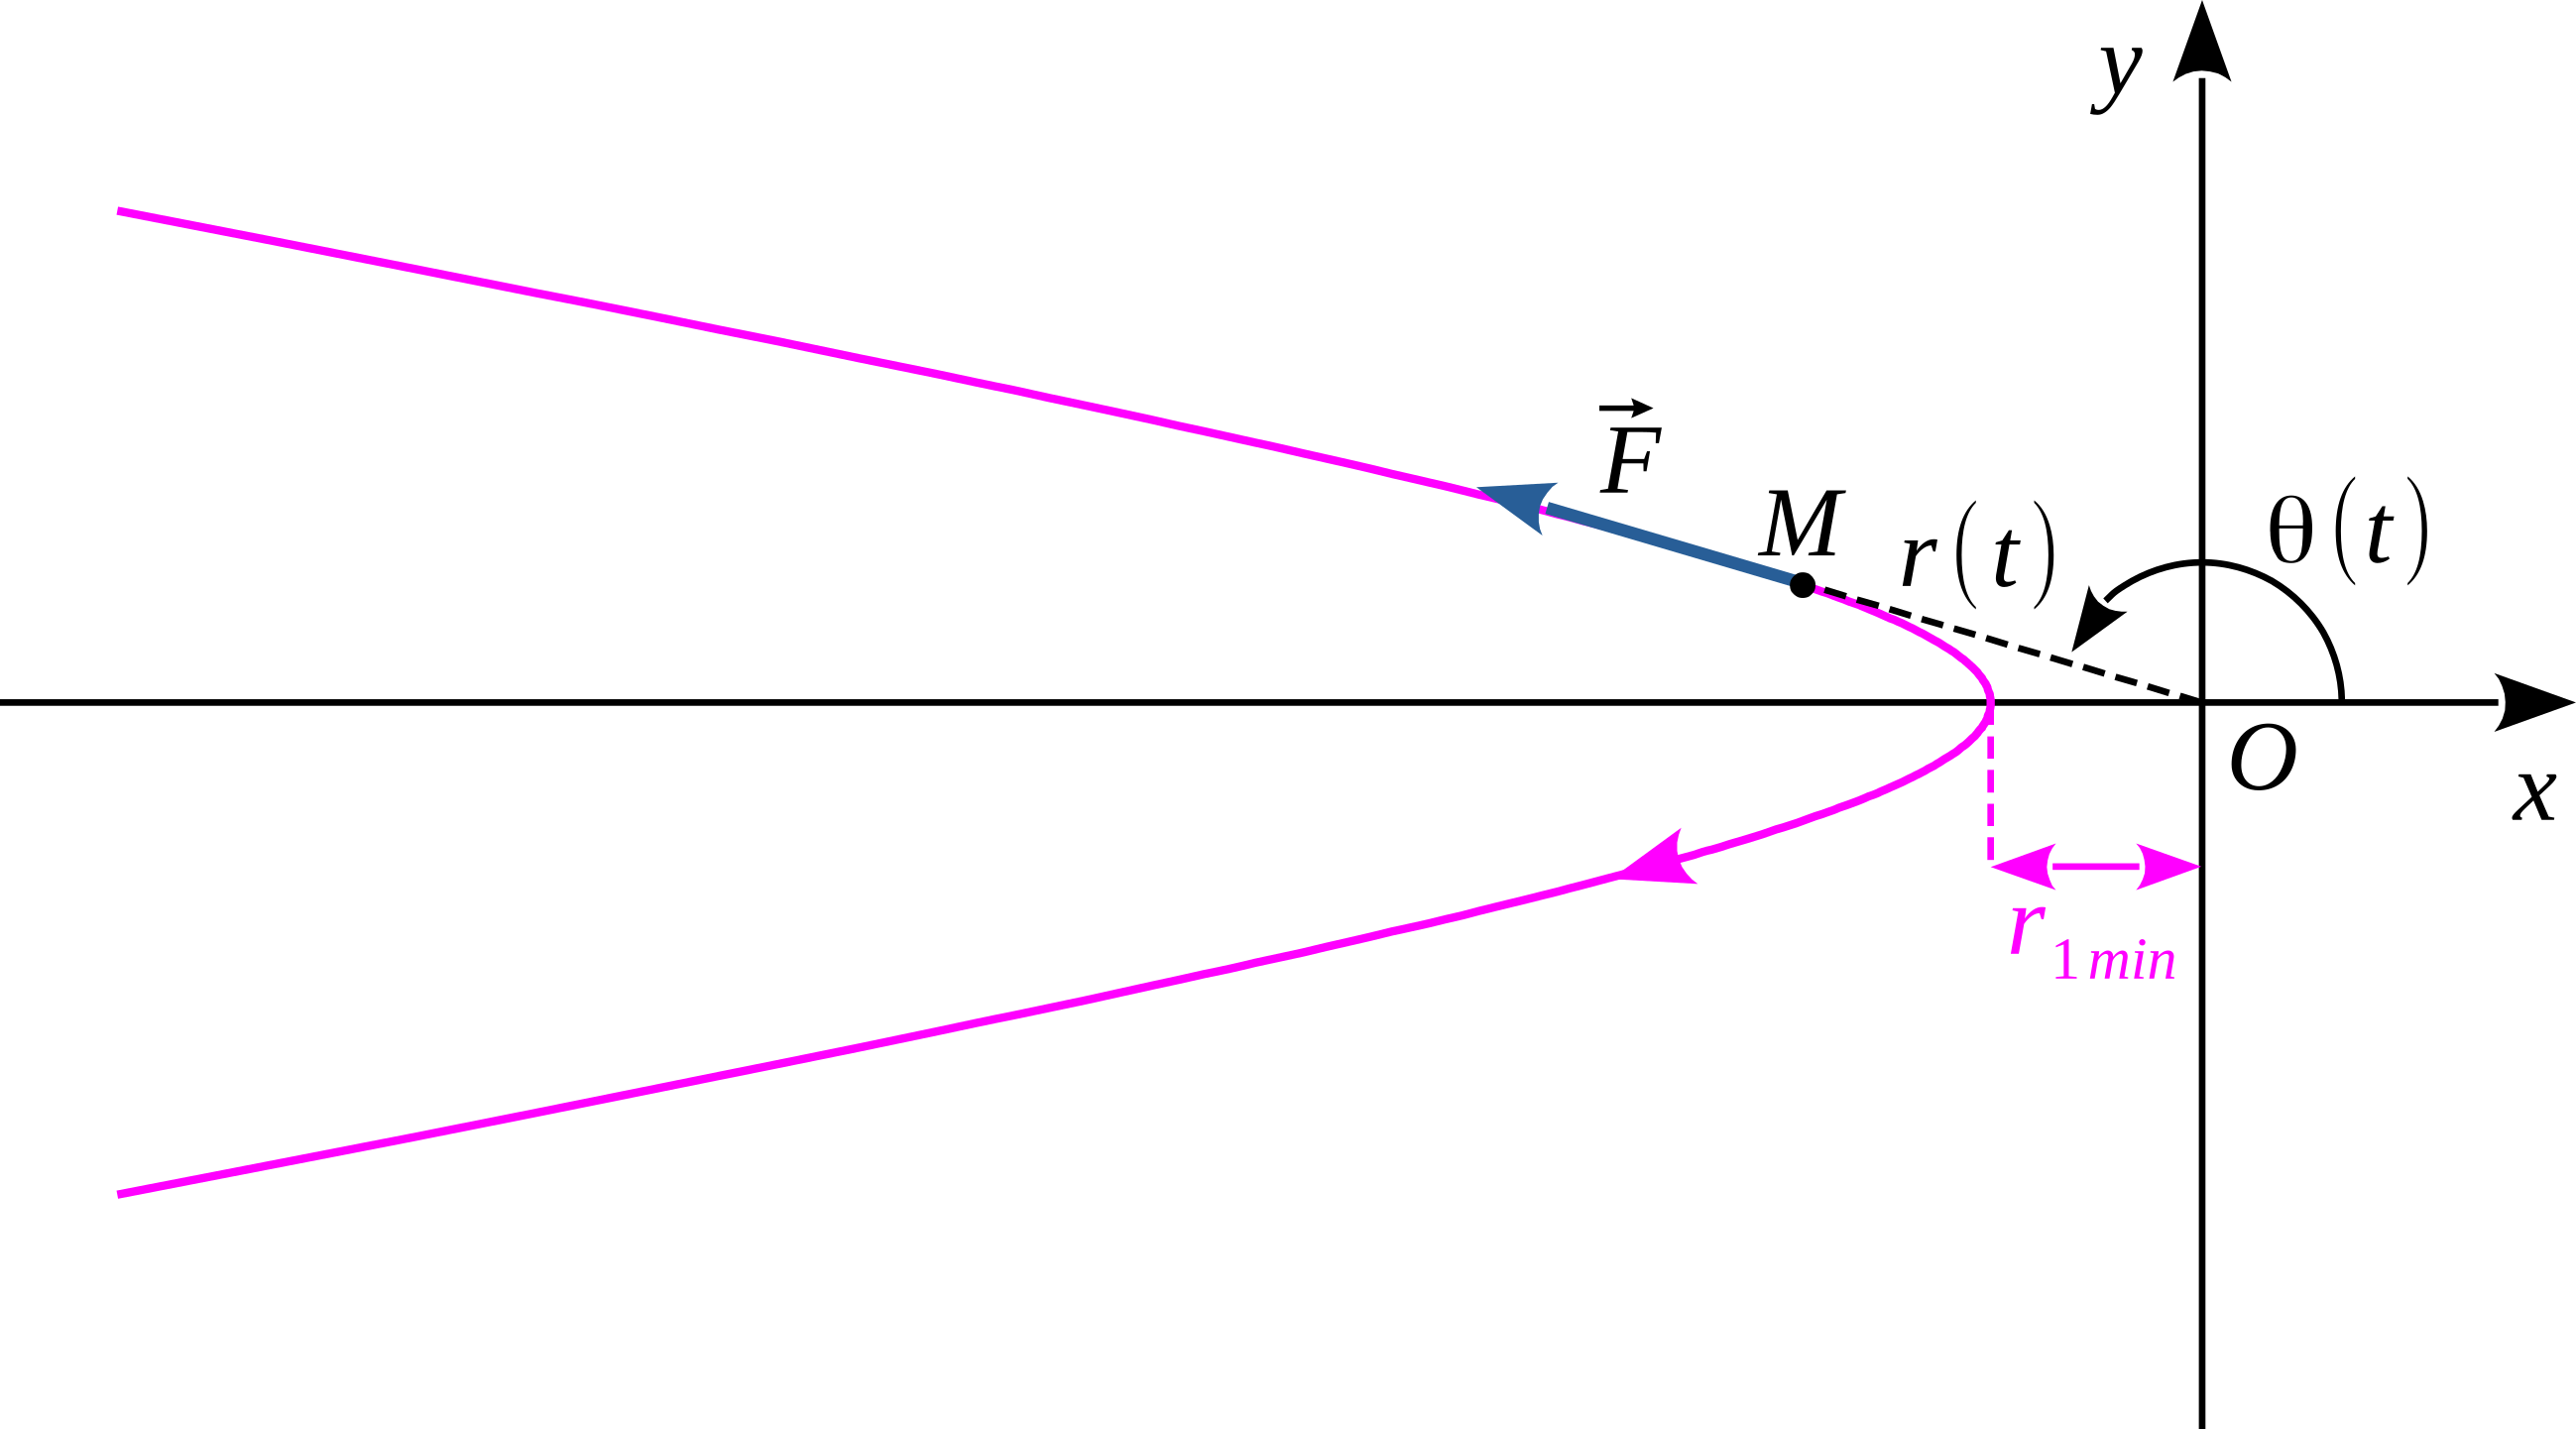
\includegraphics[height=5cm]{traj_rep-color}
		\captionof{figure}{Trajectoire cas répulsifs.}
	\end{center}
\end{minipage}

\section{Mécanique céleste}
\subsection{Qu'est-ce qu'une ellipse~?}
\begin{tcb*}(defi){Ellipse}
	\begin{isd}[righthand ratio=.45]
		Une ellipse se définit comme l'ensemble des points M tels que
		\[\boxed{\psw{{\rm MF}+{\rm MF'} = 2a}}\]
		avec F et F' les \textbf{foyers} de l'ellipse, et son $a$ demi-grand axe.
		\smallbreak
		Le point le plus proche s'appelle le \textbf{péricentre}\footnote{Périgée
			pour la Terre, périhélie pour le Soleil}~P, et le plus éloigné
		s'appelle l'\textbf{apocentre}\footnote{Apogée pour la Terre, aphélie pour
			le Soleil}, A.
		\tcblower
		\begin{center}
      \sswitch{
        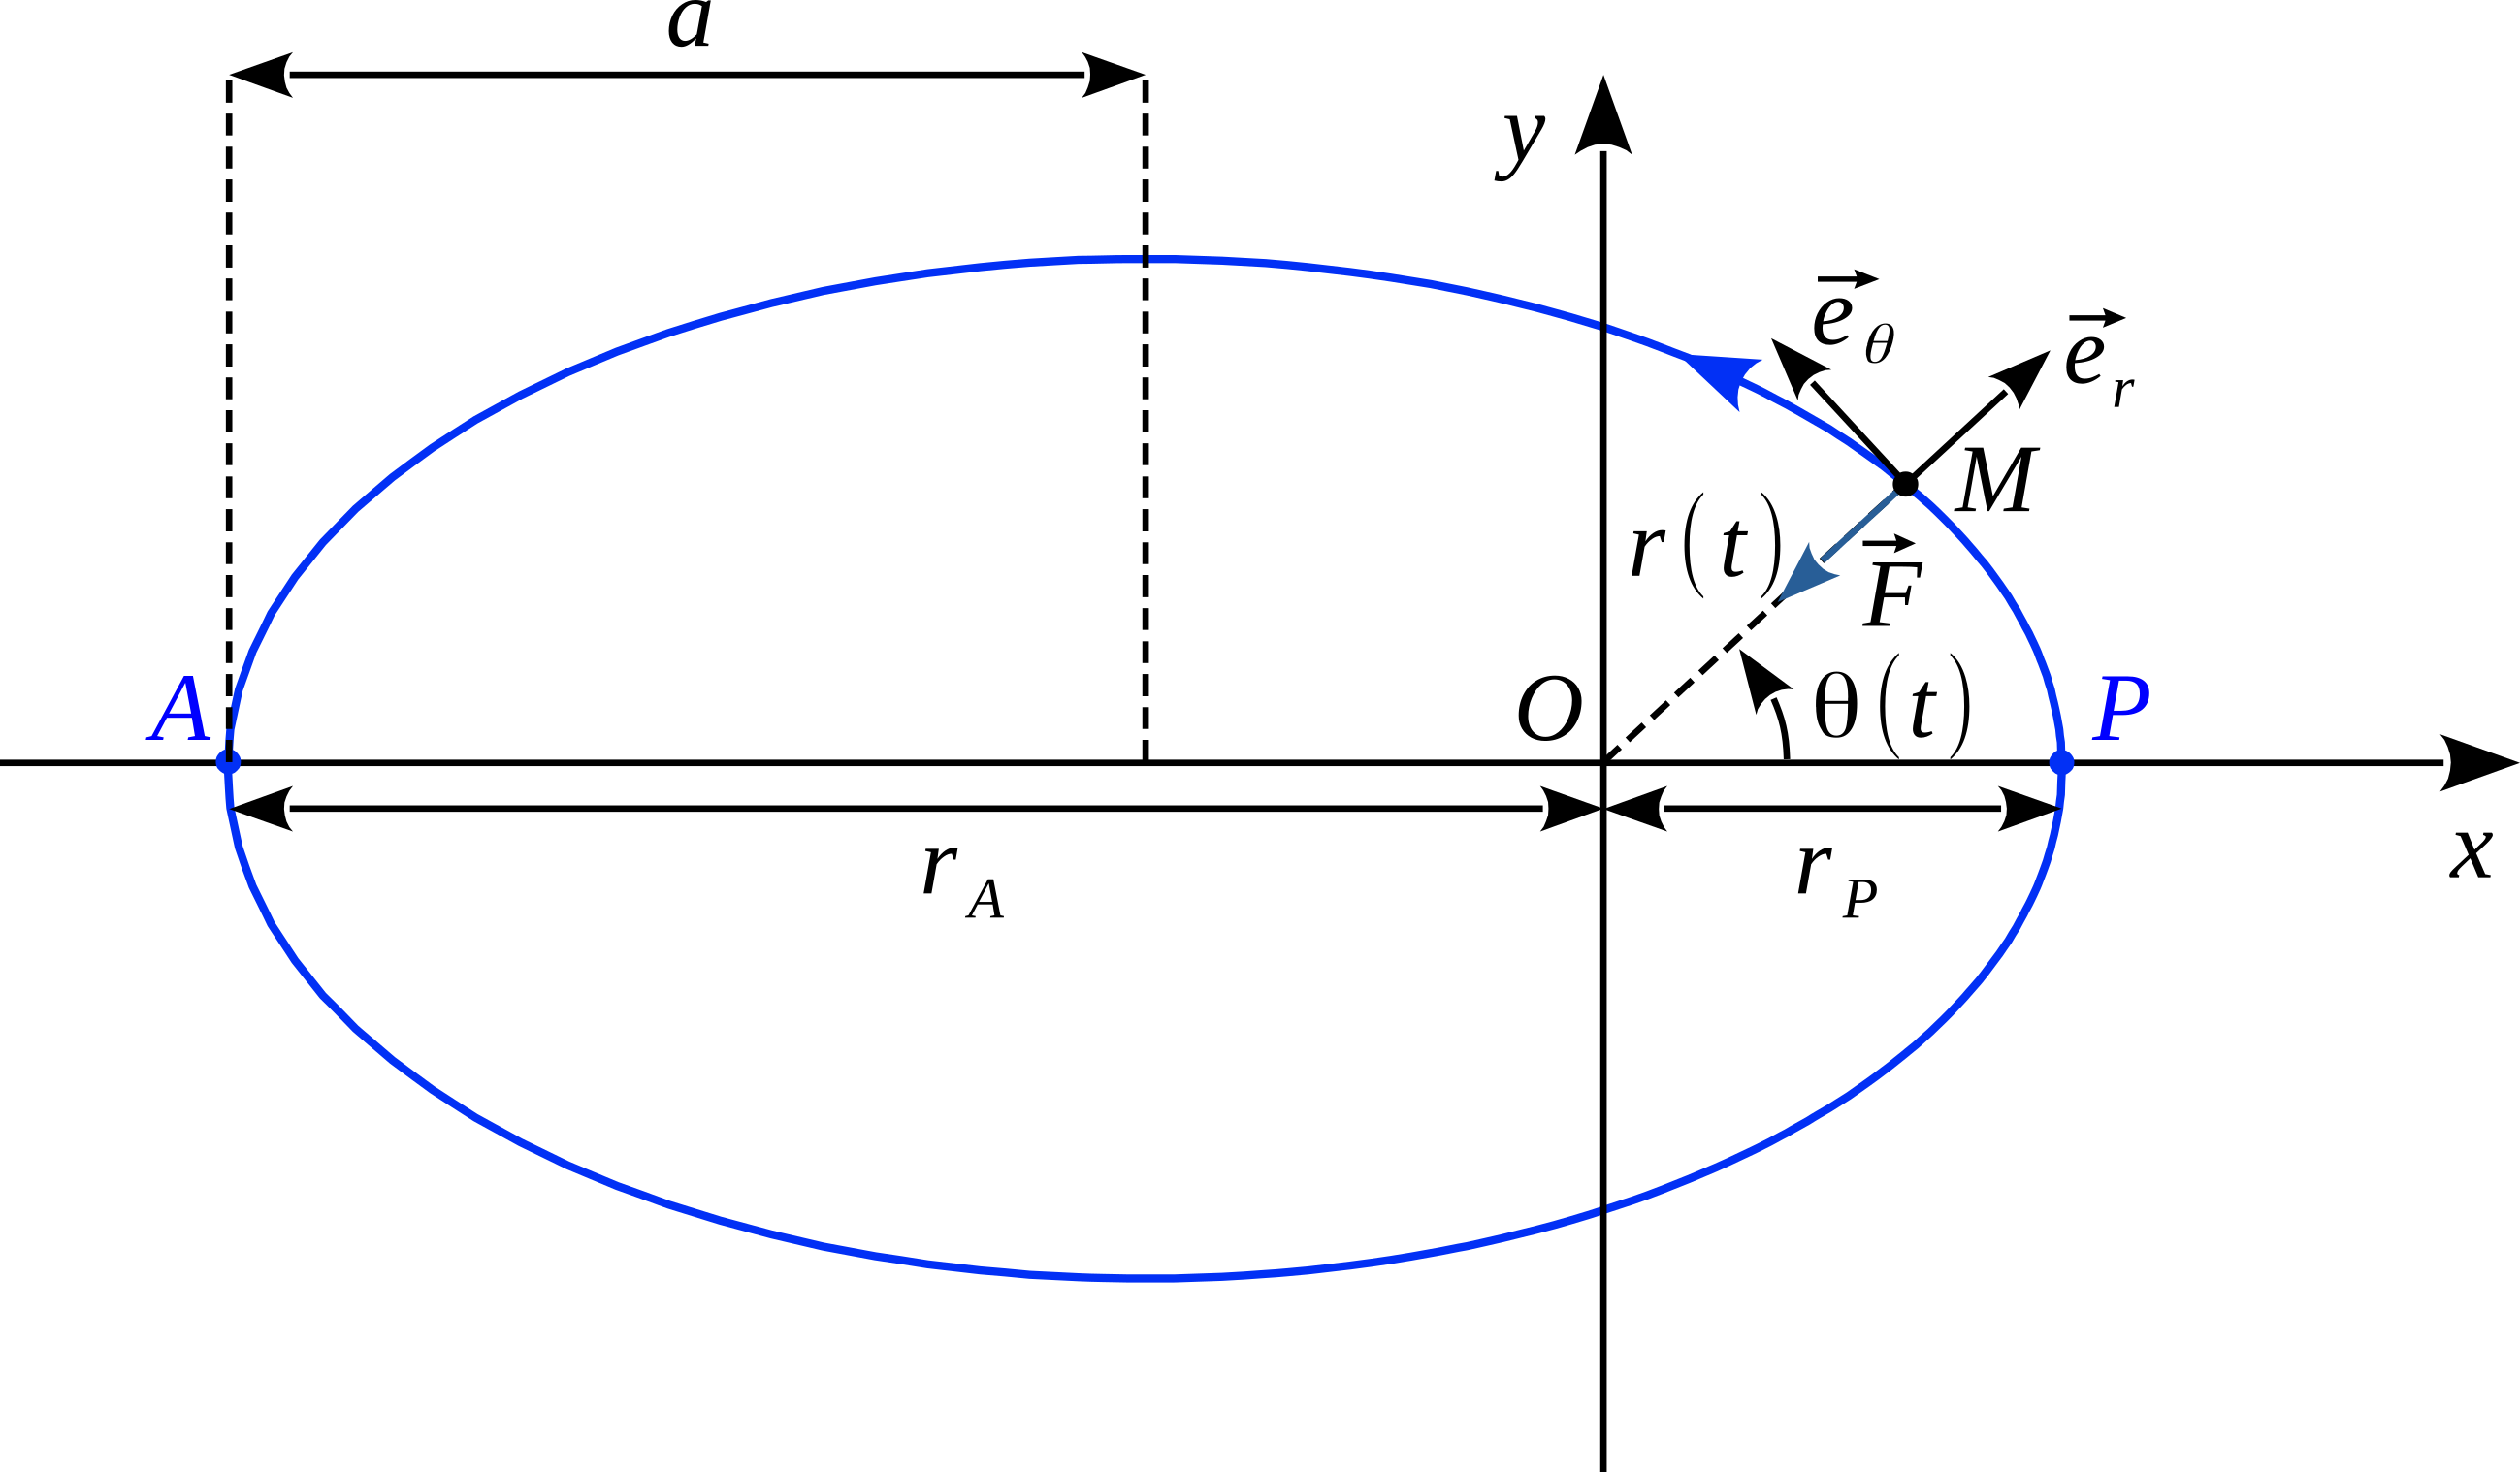
\includegraphics[width=\linewidth, draft=true]{ell_def}
      }{
			  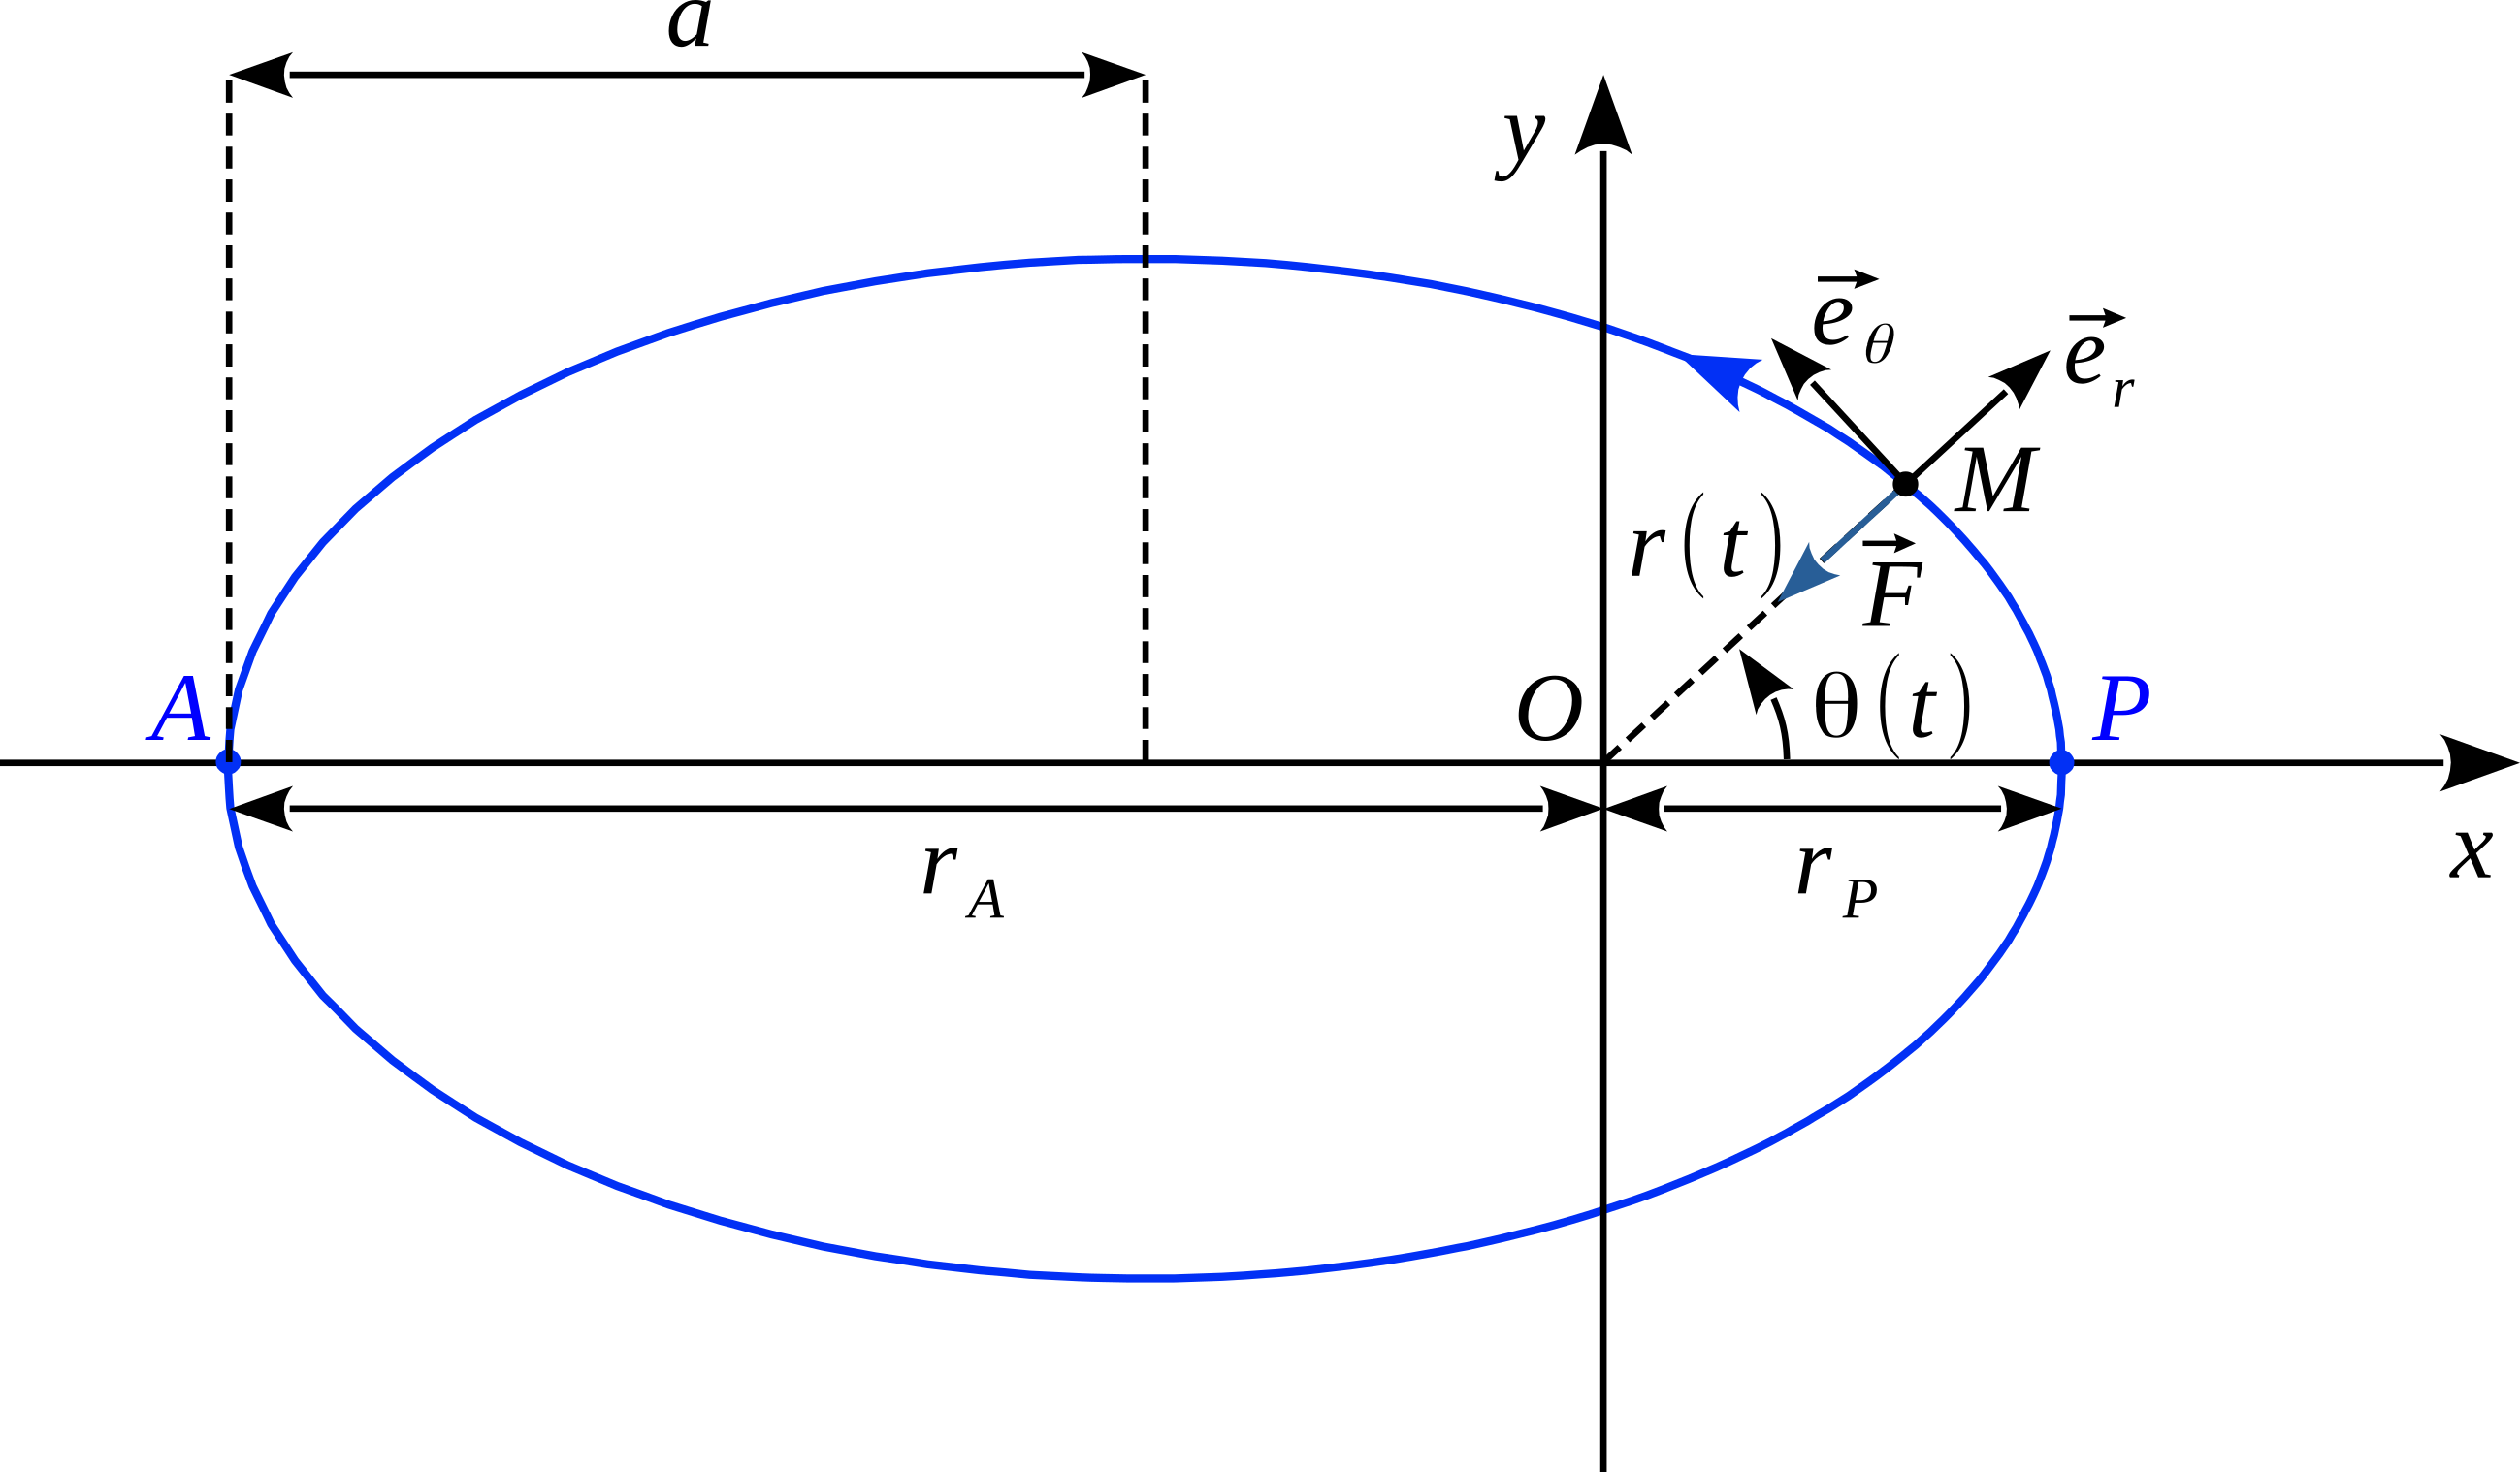
\includegraphics[width=\linewidth]{ell_def}
      }
			\captionof{figure}{Ellipse et paramètres}
		\end{center}
	\end{isd}
	\begin{itemize}
		\item Les rayons $r\ind{P}$ et $r\ind{A}$ sont reliés à $a$ tels que
		      \psw{$\boxed{r\ind{P} + r\ind{A} = 2a}$}~;
		      \vspace{-10pt}
		\item Par construction, P et A sont à des extremum de rayon, soit
		      $\rp\ind{P|A} = 0 \Lra \psw{\boxed{\vf\ind{P|A} = r\ind{P|A}\tp \et}}$
	\end{itemize}
\end{tcb*}

\subsection{Lois de \textsc{Kepler}}
Les lois de \textsc{Kepler} ont été établies par Johannes \textsc{Kepler} au
début du \textsc{xvii}\ieme\ siècle (publiées en 1609 et 1619) à partir de
relevés expérimentaux effectués par Tycho \textsc{Brahe} à la fin du
\textsc{xvi}\ieme\ siècle.
% \bigbreak
% La première loi de \textsc{Kepler} précise la nature des trajectoires des
% planètes.
\begin{tcb*}[sidebyside](loi){Lois de \textsc{Kepler}}
	\begin{enumerate}
		\bitem{Loi des orbites}~:
		\psw{les planètes ont des trajectoires elliptiques dont le Soleil occupe un
			des foyers~;}
		\vspace{20pt}
		\bitem{Loi des aires}~:
		\psw{pendant une durée donnée $\Dt$, l'aire $\D\Ac$ balayée par une planète
			est constante.}
		\vspace{20pt}
		\bitem{Loi des périodes}~:
		\psw{
			La période de révolution d'une planète autour du Soleil est reliée au
			demi-grand axe de son ellipse par~:
			\[
				\boxed{
					\frac{T^2}{a^3} = \cte
					\ftn{Plus précisément,
						$\frac{T^2}{a^3} = \frac{4\pi^2}{\Gc M_\Sr}$}
				}
			\]
		}
	\end{enumerate}
	\tcblower
	\begin{center}
		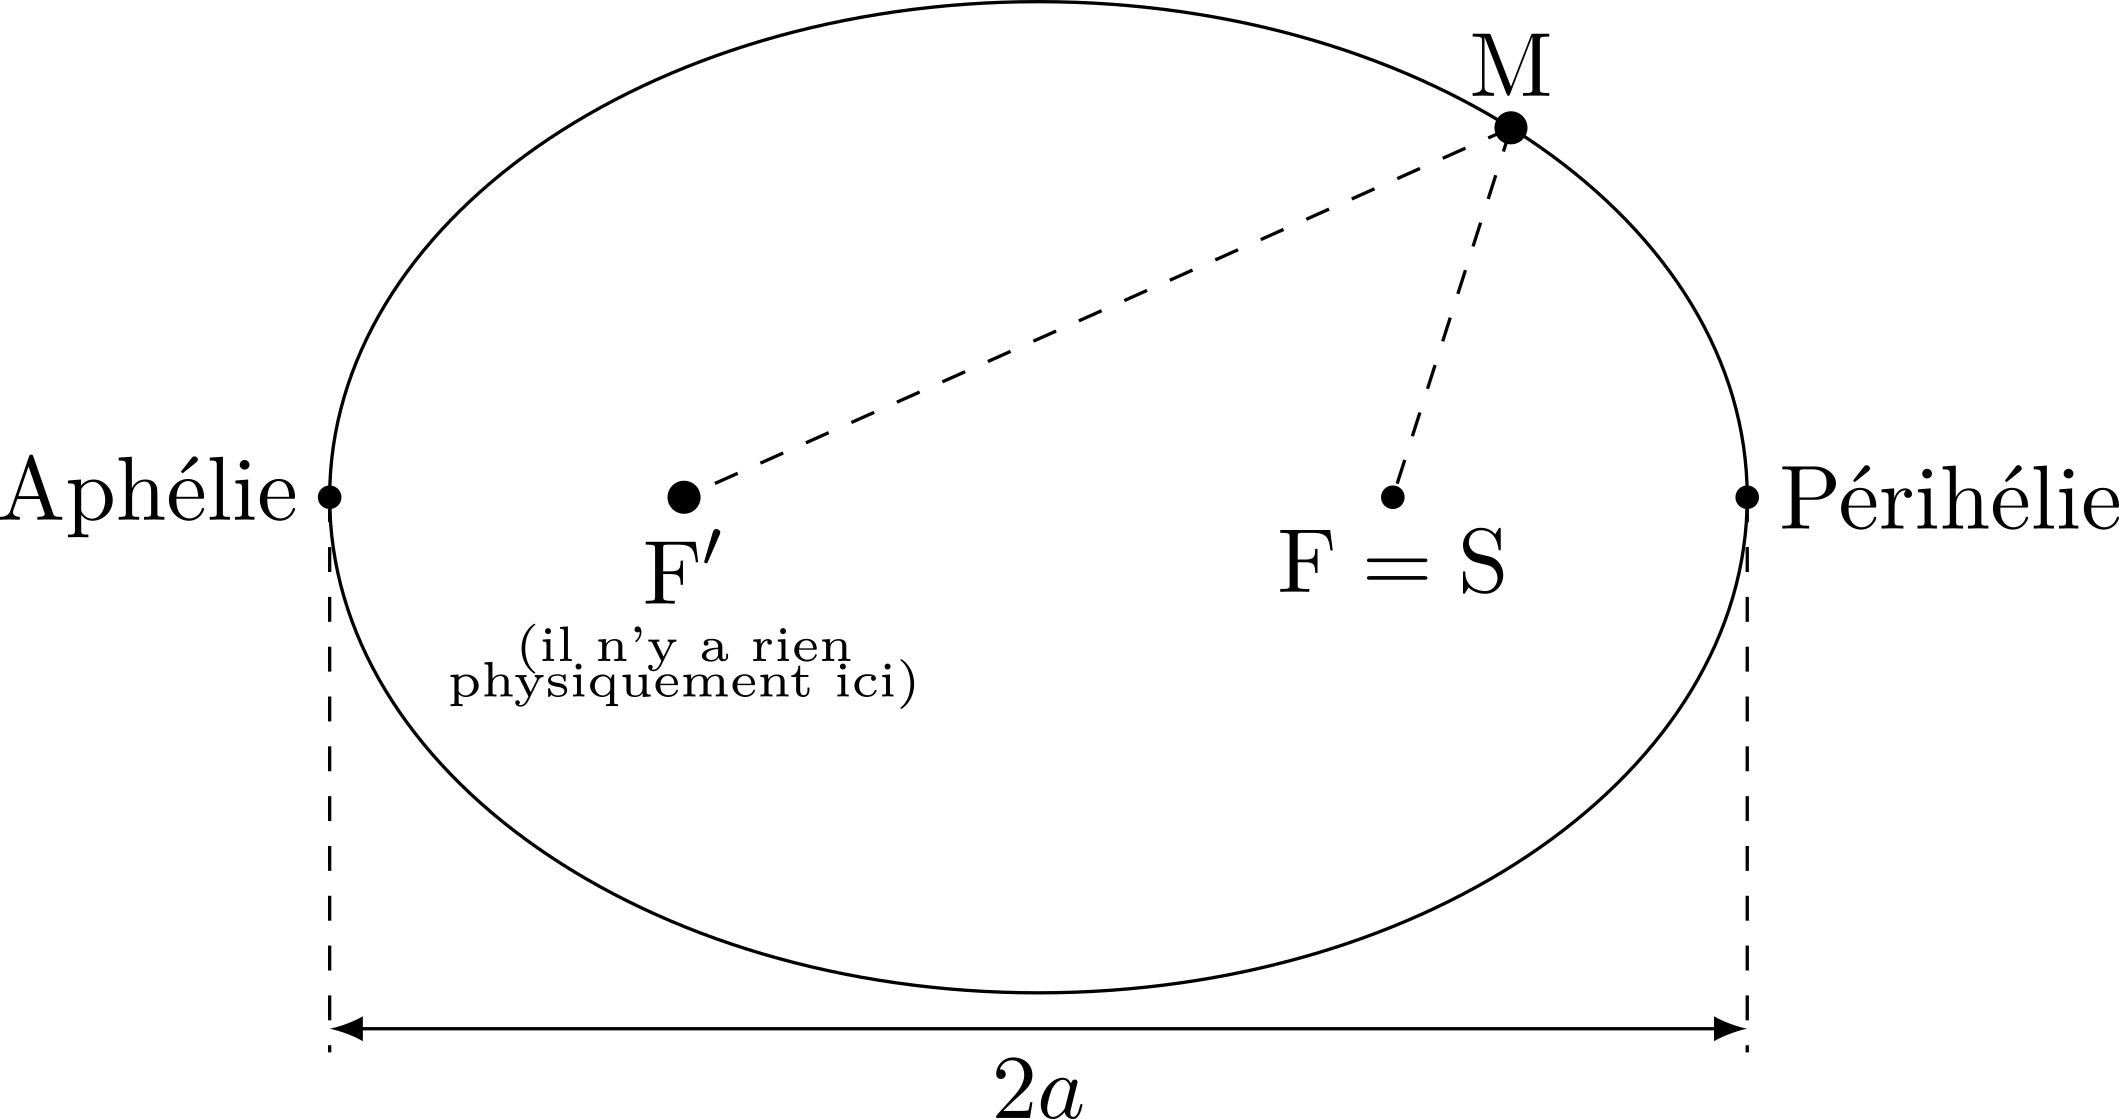
\includegraphics[width=\linewidth]{kepler_1}
		\captionof{figure}{1\iere{} loi de \textsc{Kepler}}
	\end{center}
	\begin{center}
		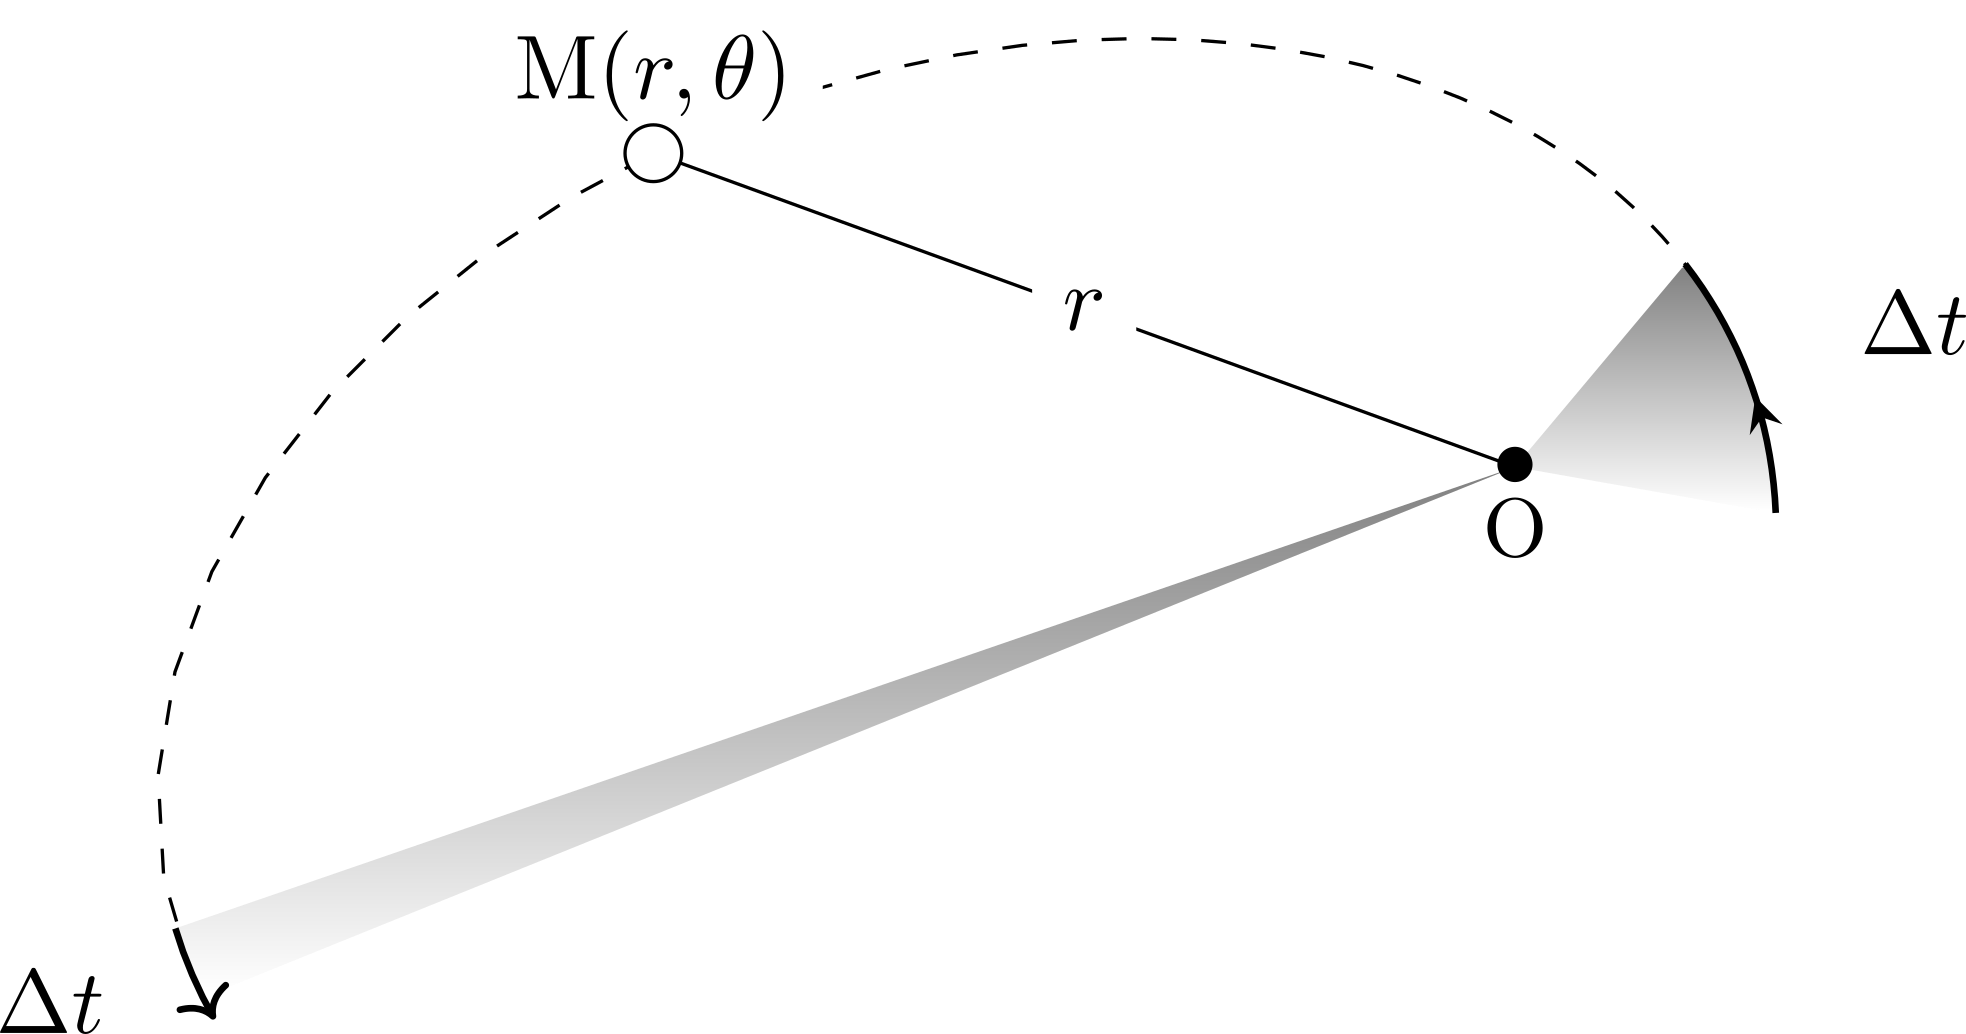
\includegraphics[width=.8\linewidth]{kepler_2-aire.png}
		\captionof{figure}{2\ieme{} loi de \textsc{Kepler}}
	\end{center}
\end{tcb*}

\begin{tcb*}(appl)<lftt>'l'{Troisième loi de \textsc{Kepler}}
	Calculer la période de révolution de Mars autour du Soleil. On donne $a_{\rm
				Terre} = \SI{150e6}{km}$ et $a_{\rm Mars} = \SI{228e6}{km}$.
	\tcblower
	\psw{
		\begin{gather*}
			\frac{T_\Mr{}^2}{a_\Mr{}^3} =
			\frac{4\pi^2}{\Gc M_\Sr} =
			\frac{T_\Ter{}^2}{a_\Ter{}^3}
			\\\Lra
			\boxed{T_\Mr = T_\Ter \sqrt{\frac{a_\Mr{}^3}{a_\Ter{}^3}}}
			\qavec
			\left\{
			\begin{array}{rcl}
				T_\Ter & = & \SI{1}{an}     \\
				a_\Ter & = & \SI{150e6}{km} \\
				a_\Mr  & = & \SI{228e6}{km}
			\end{array}
			\right.
			\\\AN
			\boxed{T_\Mr = \SI{1}{an}\,\SI{319}{jours}}
		\end{gather*}
	}
	\vspace{-30pt}
\end{tcb*}

\subsection{Cas particulier du mouvement circulaire et généralisation}
\subsubsection{Vitesse uniforme}
\begin{tcb*}[sidebyside, righthand ratio=.35](ror){Vitesse des orbites
			circulaires}
	\begin{bfseries}
		Le mouvement \ul{circulaire} d'un astre autour d'un autre
		est nécessairement uniforme, et on a
	\end{bfseries}
	\tcblower
	\psw{\[\boxed{v\ind{cercle} = \sqrt{\frac{\Gc M_S}{R}}}\]}
\end{tcb*}

\begin{tcb*}(demo)<lftt>{Démonstration vitesse circulaire}
	\noindent
	\begin{minipage}[t]{0.70\linewidth}
		\begin{enumerate}[label=\sqenumi]
			\bitem{Système}~: \psw{\{planète\} point matériel M de masse $m$}
			\bitem{Référentiel}~: \psw{
				héliocentrique, supposé galiléen.
			}
			\bitem{Repère}~: \psw{
				polaire $(\Or,\ur,\ut)$ avec O centre du Soleil, R le
				rayon supposé constant ($\dot{R} = 0$).
			}
			\bitem{Repérage}~:
			\vspace{-15pt}
			\begin{align*}
				\OM & = \psw{R\ur}                  \\
				\vf & = \psw{R\tp\ut}               \\
				\af & = \psw{-R\tp^2\ur + R\tpp\ut}
			\end{align*}
			\bitem{Bilan des forces}~:
			\psw{$\DS\Ff_g = -\Gc \frac{mM_S}{R^2}\ur$ avec $M_S$ la masse du soleil.
			}
		\end{enumerate}
	\end{minipage}
	\hfill
	\begin{minipage}[t]{0.25\linewidth}
		~\vspace*{-20pt}
		\begin{center}
			\sswitch{
				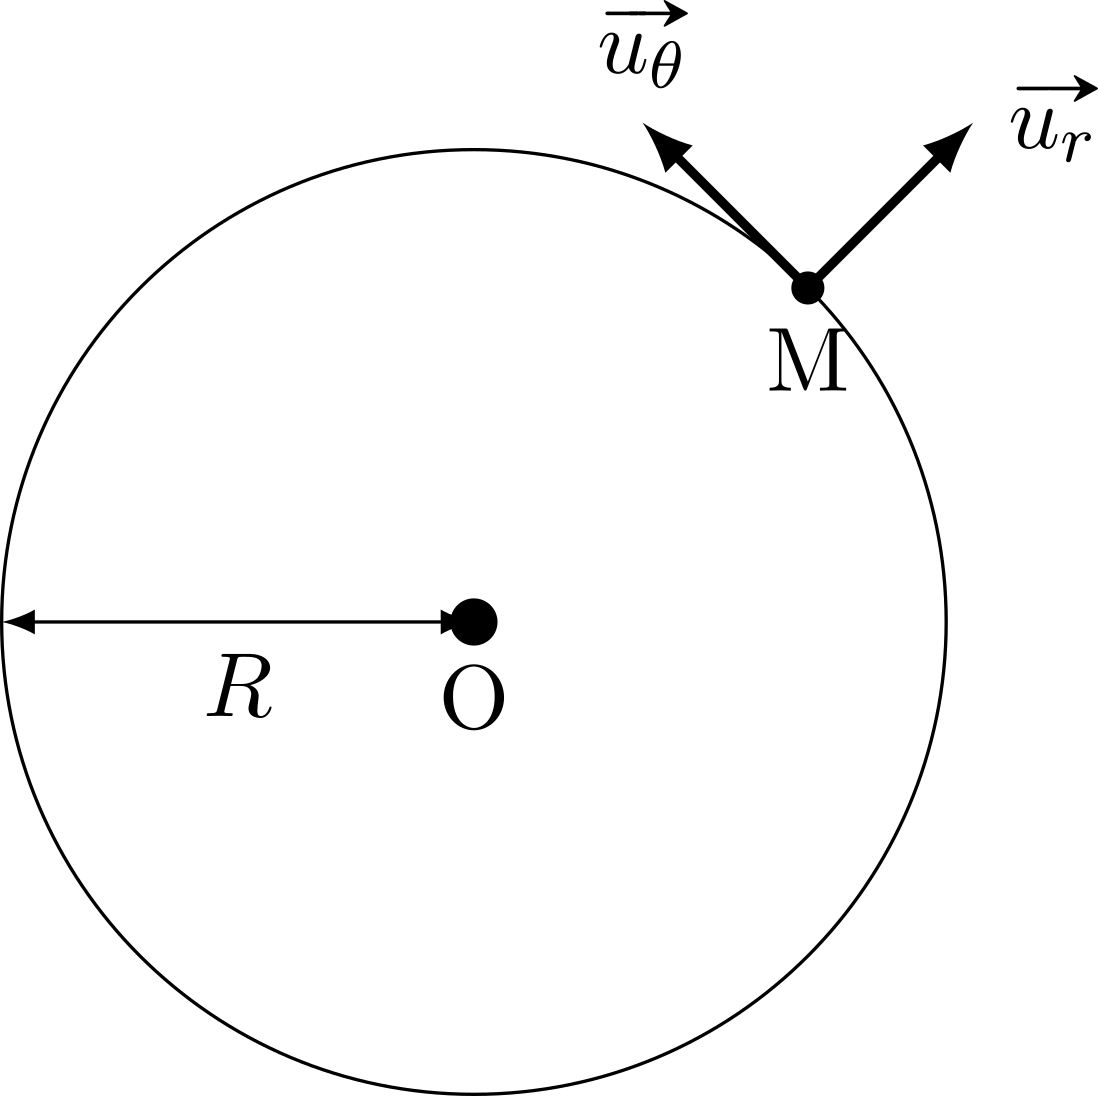
\includegraphics[width=\linewidth, draft=true]{kepler_3_circ}
			}{
				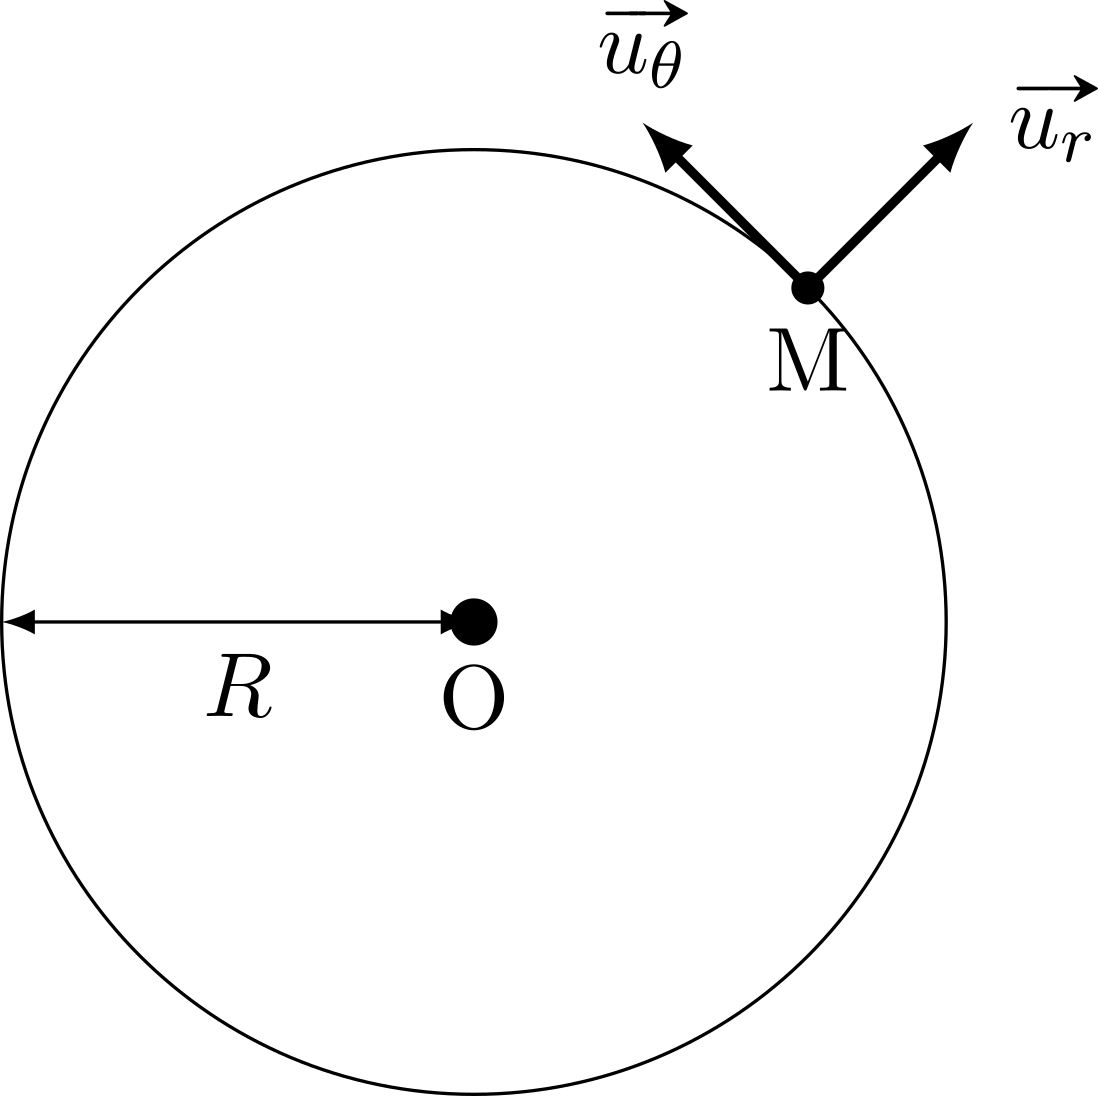
\includegraphics[width=\linewidth]{kepler_3_circ}
			}
			\captionof{figure}{Orbite circulaire.}
		\end{center}
	\end{minipage}
	\begin{enumerate}[label=\sqenumi, start=5]
		\bitem{PFD}~:
		\begin{DispWithArrows}< \psw{m\af = \Ff} \Lra >
			\psw{-mR\tp^2} &= \psw{-\Gc \frac{mM_S}{R^2}\ur}
			\label{eq:ivc71}
			\\
			\psw{mR\tpp} &= \psw{0}
			\label{eq:ivc72}
		\end{DispWithArrows}
		\bitem{Vitesse du mouvement circulaire}~:
		l'équation~\eqref{eq:ivc72} donne $\tpp = 0 \Ra \tp = \cte$,
		et~\eqref{eq:ivc71} donne
		\begin{equation}
			\psw{\boxed{\tp = \sqrt{\frac{\Gc M_S}{R^3}}}}
			\Lra
			\psw{\boxed{v = \sqrt{\frac{\Gc M_S}{R}}}}
			\rlap{$\qquad\blacksquare$}
			\label{eq:ivc73}
		\end{equation}
	\end{enumerate}
\end{tcb*}

\begin{tcb*}[cnt, bld](impo){Vitesse des orbites elliptiques}
	Le mouvement elliptique \textbf{n'est pas uniforme}~!
\end{tcb*}

\subsubsection{Période}

\begin{tcbraster}[raster equal height=rows, raster columns=2]
	\begin{tcb*}(ror){Période circulaire}
		\begin{bfseries}
			La période de révolution du mouvement \ul{circulaire} d'un astre
			autour d'un autre vérifie
			\psw{\[\boxed{\frac{T^2}{R^3} = \frac{4\pi^2}{\Gc M_S}}\]}
		\end{bfseries}
		\vspace{-15pt}
		\tcblower
		On admet que \textbf{le résultat s'étend à une trajectoire elliptique en
			remplaçant le rayon $R$ par le demi-grand axe $a$}.
	\end{tcb*}
	\begin{tcb*}(demo)<rgtt>'r'{Période circulaire}
		En effet, avec~\eqref{eq:ivc73} et $T$ la période de révolution de l'astre,
		on a
		\begin{DispWithArrows*}
			\psw{\tp}                     & = \psw{\frac{2\pi}{T}}
			\Arrow{$\tp = \sqrt{\frac{\Gc M_S}{R^{3}}}$}
			\\\Lra
			\psw{\frac{4\pi^2}{T^2}}      & = \psw{\frac{\Gc M_S}{R^3}}
			\\\Lra
			\Aboxed{\psw{\frac{T^2}{R^3}} & = \psw{\frac{4\pi^2}{\Gc M_S}}}
			\qed
		\end{DispWithArrows*}
	\end{tcb*}
\end{tcbraster}

\subsubsection{Énergie mécanique}

\begin{tcbraster}[raster equal height=rows, raster columns=2]
	\begin{tcb*}(ror){$\Ec_m$ circulaire}
		\begin{bfseries}
			L'énergie mécanique du mouvement \ul{circulaire} d'un astre autour
			d'un autre vérifie
			\psw{\[\boxed{\Ec_{m,\rm cercle} = -\Gc\frac{mM_S}{2R}}\]}
		\end{bfseries}
		\vspace{-15pt}
		\tcblower
		On admet que \textbf{le résultat s'étend à une trajectoire elliptique en
			remplaçant le rayon $R$ par le demi-grand axe $a$}.
	\end{tcb*}
	\begin{tcb*}(demo)<rgtt>'r'{$\Ec_m$ circulaire}
		Enfin, avec~\eqref{eq:ivc73} et l'énergie mécanique, on a
		\begin{DispWithArrows*}[fleqn, mathindent=0pt]
			\Ec_m         & =
			\psw{\frac{1}{2}mR^2\tp^2 - \Gc\frac{mM_S}{R}}
			\Arrow{$R\tp = \sqrt{\frac{\Gc M_S}{R}}$}
			\\\Lra
			\Ec_m         & = \psw{\frac{1}{2}m\frac{\Gc M_S}{R} - \Gc\frac{mM_S}{R}}
			\\\Lra
			\Aboxed{\Ec_m & = \psw{-\Gc\frac{mM_S}{2R}}}
			\qed
		\end{DispWithArrows*}
	\end{tcb*}
\end{tcbraster}

\section{Satellite en orbite terrestre}
On se place ici dans le référentiel géocentrique, afin de traiter le mouvement
d'un satellite autour de la Terre.
\subsection{Vitesses cosmiques}
\subsubsection{Première vitesse cosmique}
\begin{tcbraster}[raster equal height=rows, raster columns=2]
	\begin{tcb*}(defi){1\iere{} vitesse cosmique}
		La première vitesse cosmique, ou \textit{vitesse de satellisation minimale},
		est la \textbf{vitesse minimale} à fournir à un objet situé sur Terre pour
		pouvoir le placer en orbite \textbf{circulaire} autour de la Terre.
	\end{tcb*}
	\begin{tcb*}(prop)'r'{1\iere{} vitesse cosmique}
		Sur Terre, on trouve
		% \vspace{-15pt}
		\begin{gather*}
			% \beforetext{Sur Terre, on trouve}
			\psw{
				\boxed{
					v_c = \sqrt{\frac{\Gc m_\Ter}{R_\Ter}} \approx
					\SI{8}{km.s^{-1}}
				}
			}
		\end{gather*}
	\end{tcb*}
\end{tcbraster}

\begin{tcb*}(demo)<lftt>{Première vitesse cosmique}
	Pour satelliser un corps, il faut faire varier son \textbf{énergie mécanique}
	d'un état partant \textbf{du sol} jusqu'\textbf{en orbite}. La plus petite
	énergie mécanique pour cela est celle que l'on vient de déterminer dans
	l'étude de la trajectoire circulaire. Ainsi, à partir de l'énergie mécanique
	d'un objet lancé au niveau du sol, on a
	\begin{gather*}
		\psw{\Ec_{m,\rm sol} = \frac{1}{2}mv_c{}^2 -\Gc \frac{mM_\Ter}{R_\Ter}}
		\qet
		\psw{\Ec_{m,\rm cercle} = -\Gc \frac{mM_\Ter}{2R_\Ter}}
		\\
		\beforetext{Or système conservatif $\Ra$}
		\psw{
		\frac{1}{2}mv_c{}^2 -\Gc \frac{mM_\Ter}{R_\Ter} =
		-\Gc \frac{mM_\Ter}{2R_\Ter}
		}
		\\\Lra
		\psw{
			\boxed{v_c = \sqrt{\frac{\Gc m_\Ter}{R_\Ter}}}
		}
		\qed
	\end{gather*}
	Pour des altitudes plus élevées, il faut davantage de vitesse.
\end{tcb*}

\subsubsection{Seconde vitesse cosmique}
\begin{tcbraster}[raster equal height=rows, raster columns=2]
	\begin{tcb*}(defi){2\up{nde} vitesse cosmique}
		La seconde vitesse cosmique, ou \textit{vitesse de libération} et notée
		$v\ind{lib}$, correspond à la \textbf{vitesse minimale} à fournir à un objet
		situé sur Terre pour pouvoir \textbf{l'éloigner définitivement} de la Terre.
	\end{tcb*}
	\begin{tcb*}(prop)'r'{2\up{nde} vitesse cosmique}
		Pour la Terre, on trouve
		% \vspace{-15pt}
		\begin{gather*}
			% \beforetext{Pour la Terre, on trouve}
			\psw{
				\boxed{
					v\ind{lib} = \sqrt{\frac{2\Gc m_\Ter}{R_\Ter}} = \sqrt{2}v_c =
					\SI{11}{km.s^{-1}}
				}
			}
		\end{gather*}
	\end{tcb*}
\end{tcbraster}
\begin{tcb*}(demo)<lftt>{Seconde vitesse cosmique}
	Pour éloigner définitivement un objet de la Terre, il faut que sa trajectoire
	soit à minimum parabolique, donc que \textbf{son énergie mécanique soit
		nulle}. Ceci correspond à
	\begin{gather*}
		\psw{
			\frac{1}{2}mv\ind{lib}{}^2 -\Gc \frac{mM_\Ter}{R_\Ter} = 0
		}
		\\
		\psw{
			\Lra
			v\ind{lib} = \sqrt{\frac{2\Gc m_\Ter}{R_\Ter}}
		}
		\qed
	\end{gather*}
	\vspace{-15pt}
\end{tcb*}
La réalité est évidemment plus complexe que ça, étant donné les frottements, la
non-galiléanité des référentiels, la prise en compte de la masse de carburant
nécessaire, etc…
\begin{center}
	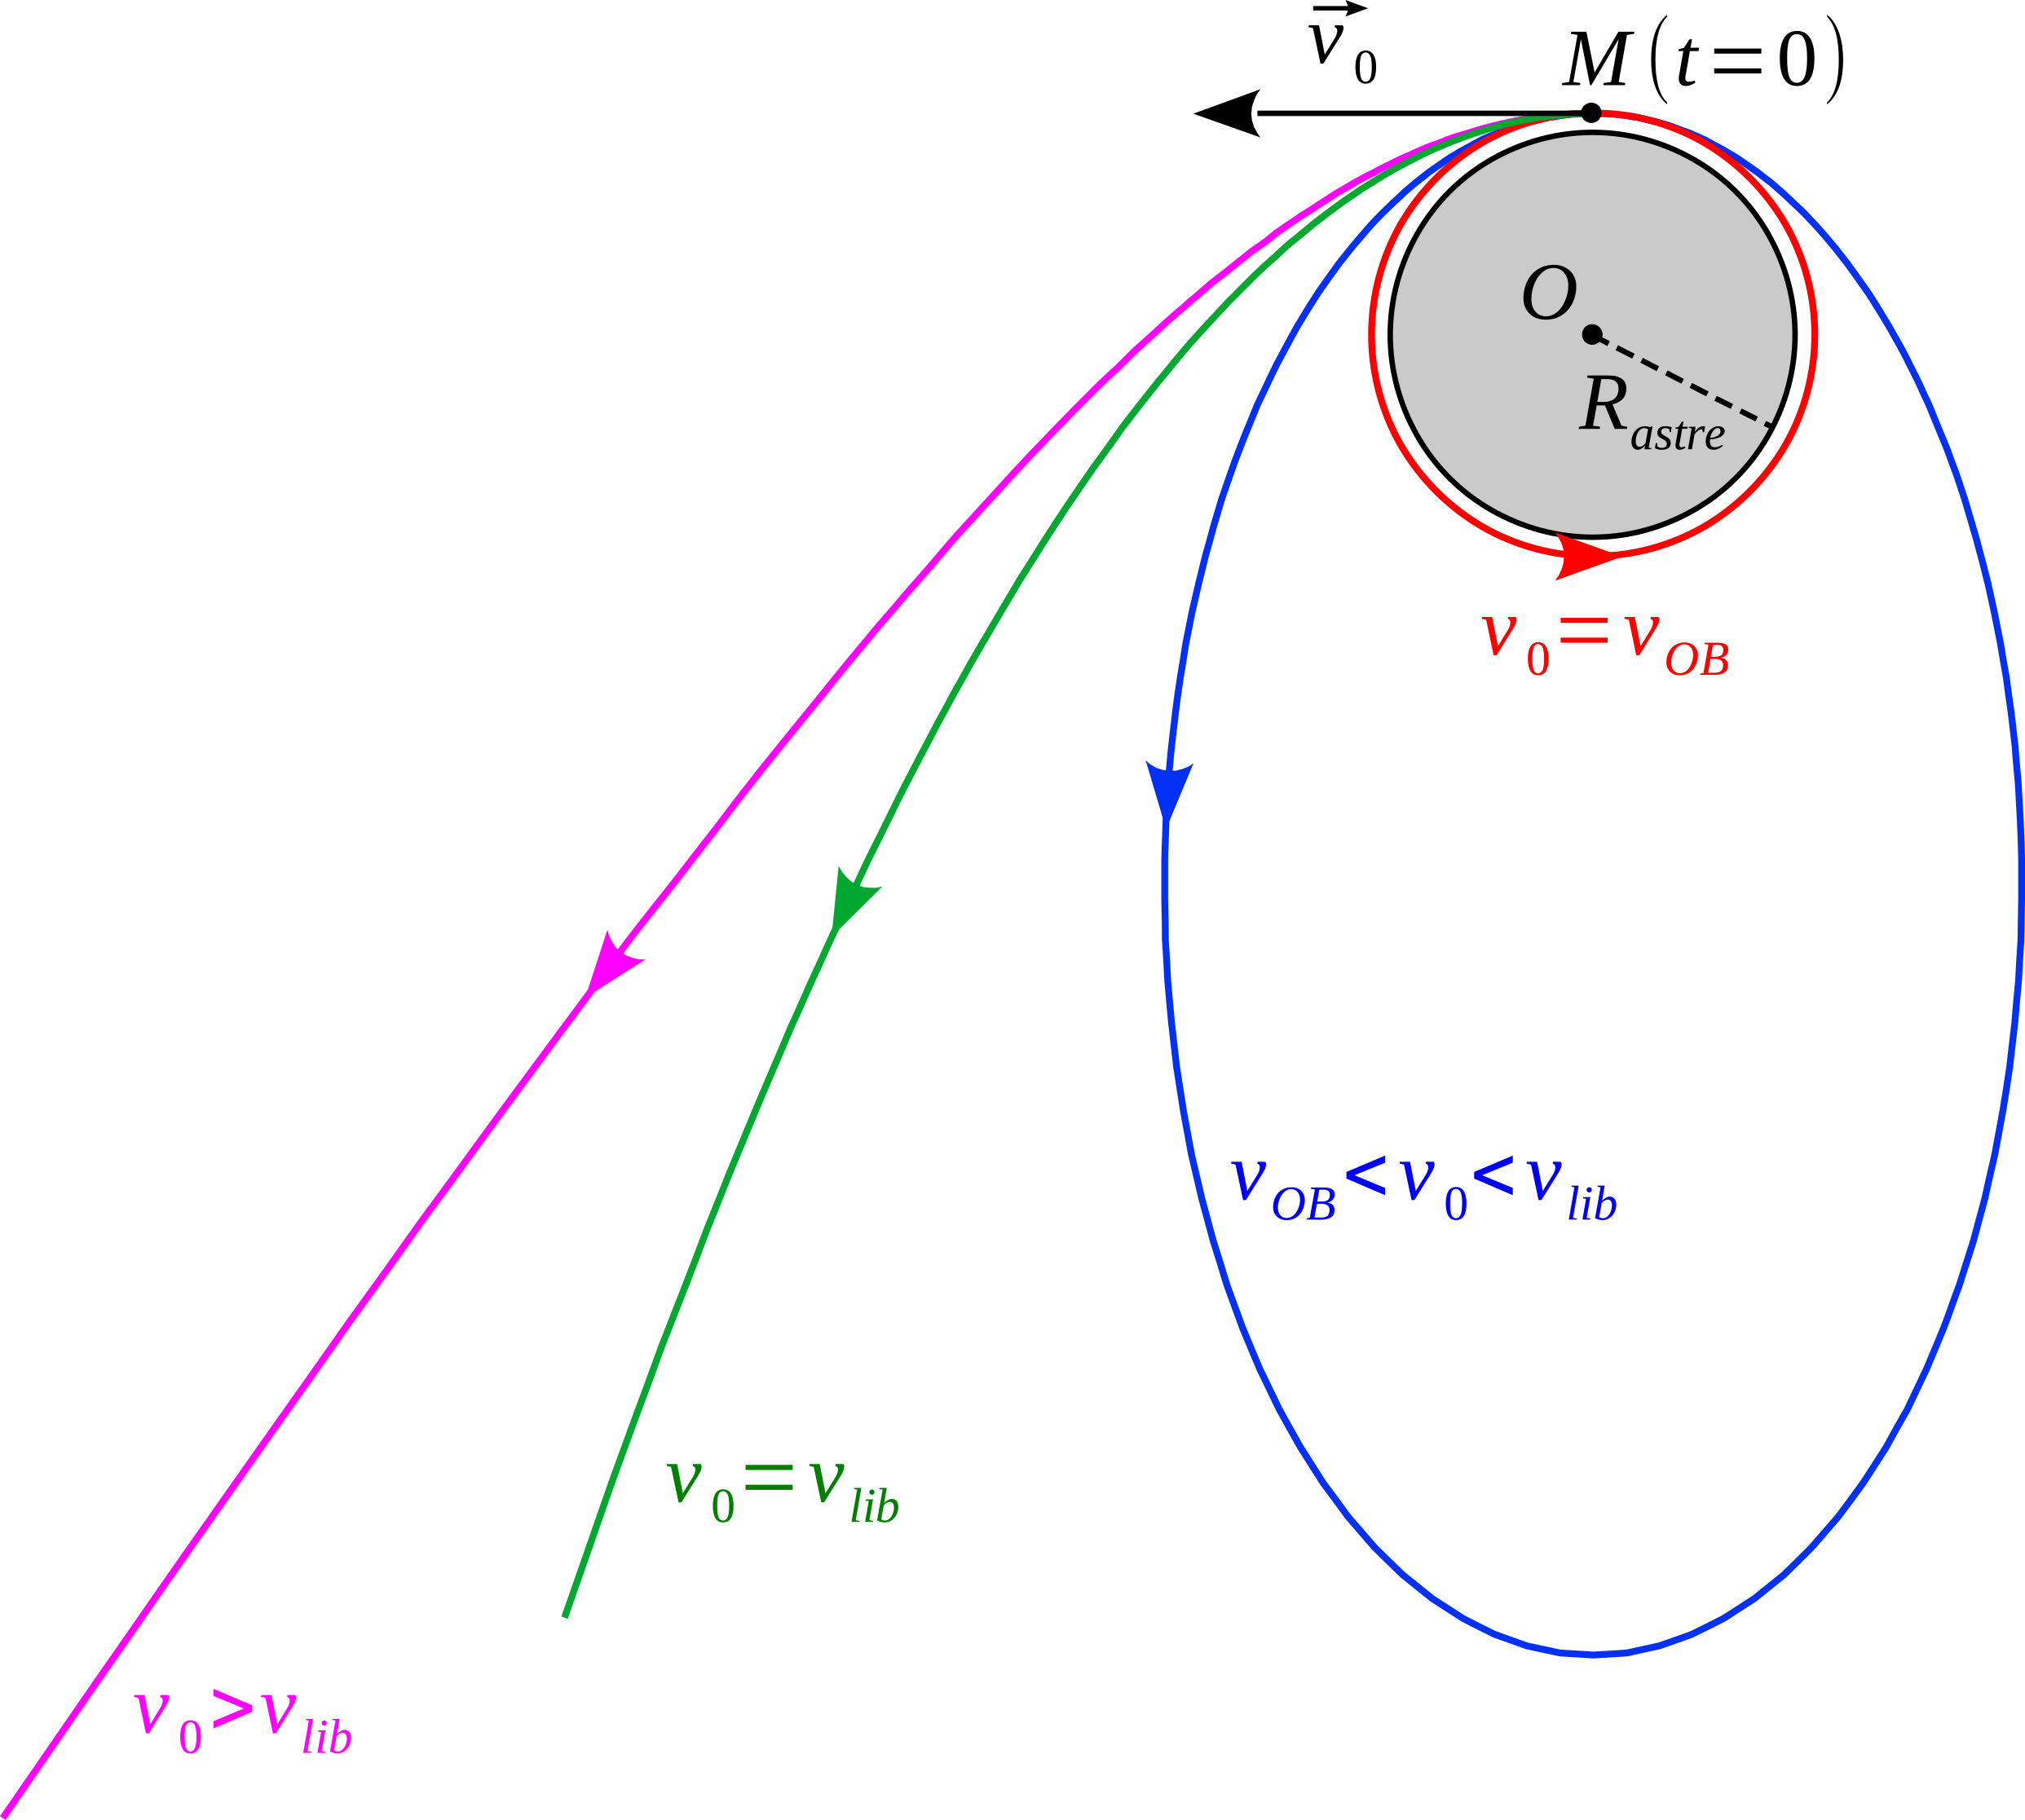
\includegraphics[scale=.7]{vit_cos}
	\captionof{figure}{Représentation des trajectoires possible pour un astre
		autour d'un autre en fonction des vitesses. Le code couleur correspond à celui
		de la Section~\fullref{--}{ssec:trajatt}.}
\end{center}

\subsection{Satellites artificiels}
\subsubsection{Satellite géostationnaires}
\begin{tcb*}[sidebyside](defi){Définition}
	Un satellite géostationnaire est un satellite qui \textbf{reste constamment
		au-dessus d'un même point} de la surface terrestre~; il apparaît donc
	immobile pour um observataire terrestre.
	\tcblower
	\textbf{Mission typique}~: obtenir des images fixes de la Terre avec une vue
	éloignée (à des fins météorologiques par exemple).
\end{tcb*}
Un tel système doit respecter trois conditions~:
\begin{enumerate}
	\bitem{Le plan de l'orbite doit être le plan de l'équateur}.
	\smallbreak
	\begin{isd}
		\begin{center}
			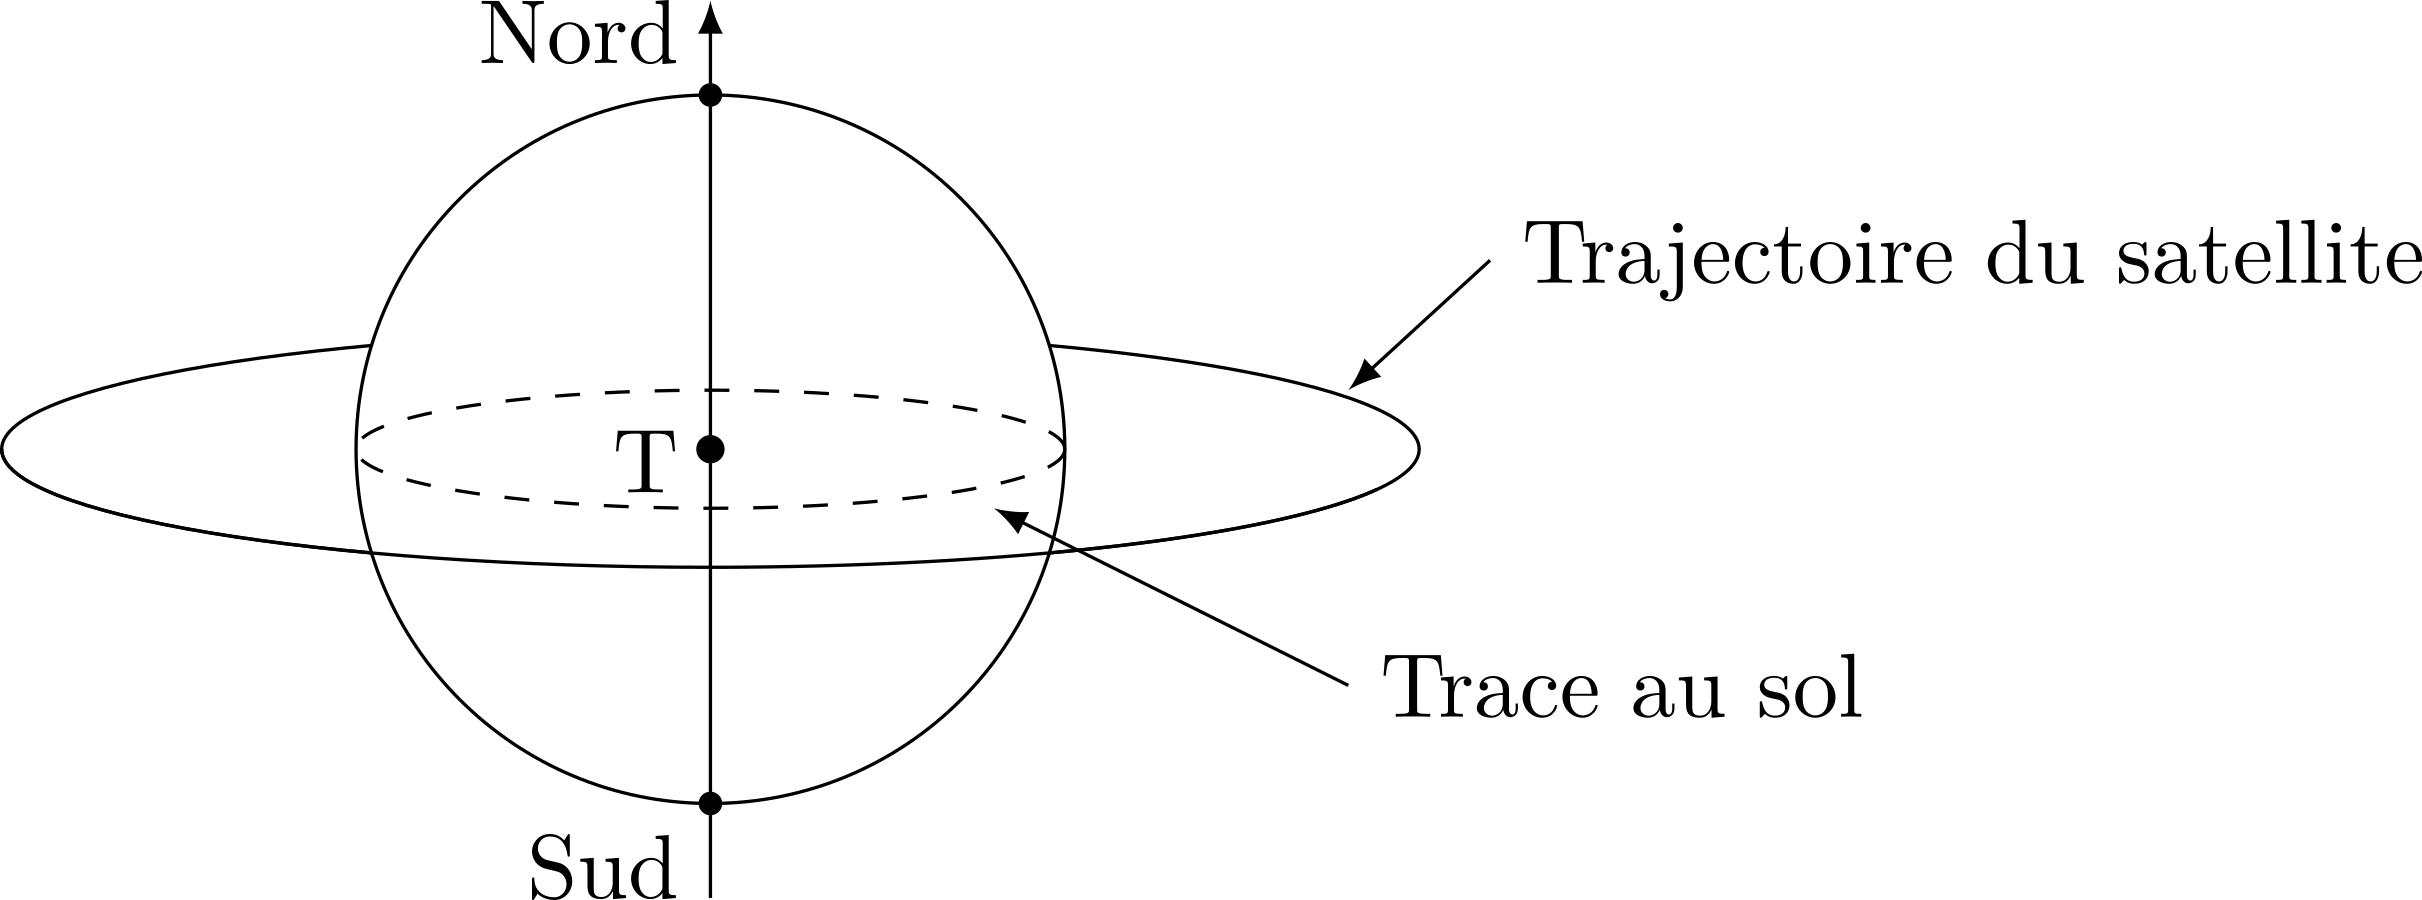
\includegraphics[width=\linewidth]{sat_geo}
		\end{center}
		\tcblower
		\begin{center}
			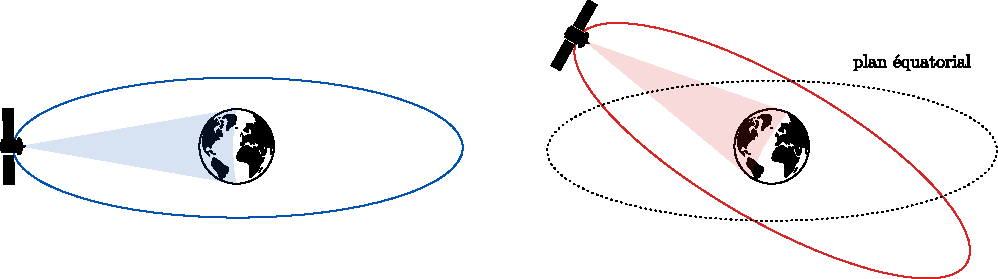
\includegraphics[width=\linewidth]{sat_geo_plan}
		\end{center}
	\end{isd}
	En effet, par principe de force centrale conservative, le mouvement est
	un plan passant par T le centre de la Terre. Mais comme la Terre est en
	rotation autour de l'axe de ses pôles, le seul plan contenant le centre
	de la Terre et permettant de rester immobile par rapport à sa surface
	est celui contenant l'équateur.
	\bitem{Le mouvement doit être synchrone avec la rotation de la Terre sur
		elle-même}. En effet d'après la raison précédente, même sur le plan de
	l'équateur il faut avoir la même vitesse angulaire $\w$, telle que
	\[\boxed{\w\ind{sat} = \tp = \w_\Ter = \frac{2\pi}{T\ind{jour}}}\]
\end{enumerate}
\begin{tcb*}[breakable](impo)<lftt>'l'{Jours solaire et sidéral}
	Il existe deux durées qui peuvent s'appeler «~jour~»~:
	\begin{itemize}
		\item le \textbf{jour sidéral}, que l'on croît à tord être celui qu'on
		      emploie au quotidien, et qui correspond à la durée nécessaire pour que
		      la Terre effectue une \textbf{rotation complète sur elle-même}~; on a
		      \[T\ind{sidéral} = \SI{23}{h}\,\SI{56}{min}\,\SI{04}{s}\]
		\item le \textbf{jour solaire} est l'intervalle de temps séparant deux
		      \textbf{passages du Soleil au zénith} d'un point donné de la Terre,
		      i.e.\ le temps qui sépare deux «~midis~» sur Terre~; on a
		      \[T\ind{solaire} = \SI{24}{h}\]
	\end{itemize}
	Ces deux notions diffèrent légèrement à cause de la révolution de la Terre
	autour du Soleil.
	\begin{center}
		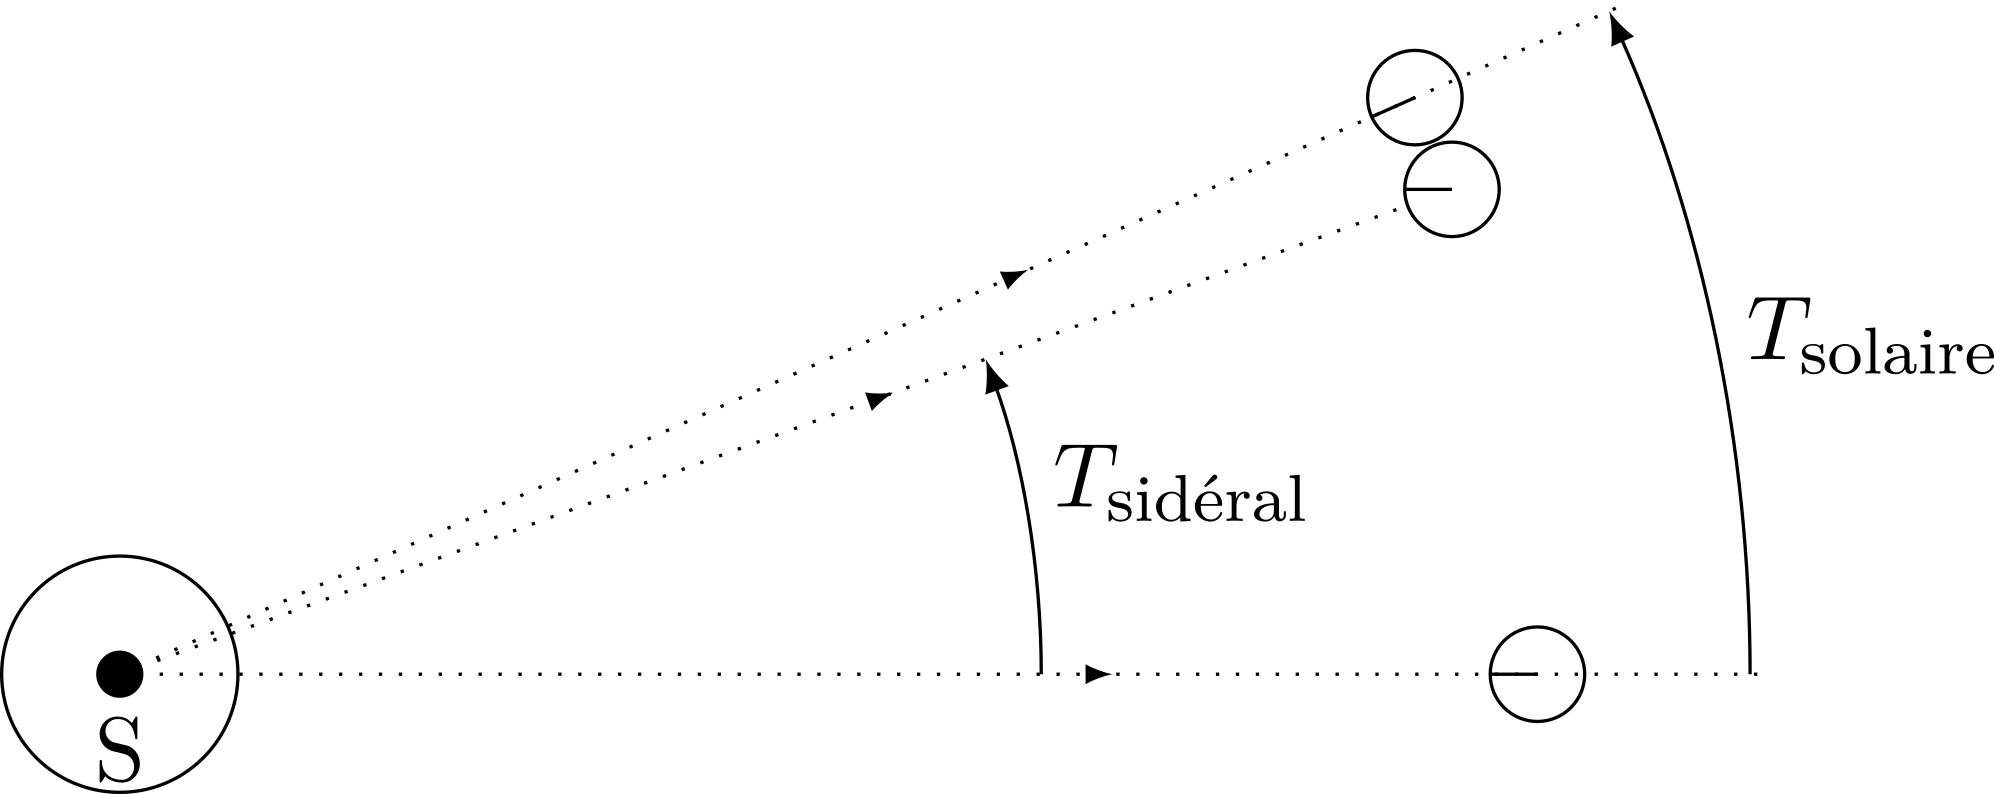
\includegraphics[scale=1]{jsid_jsol}
	\end{center}
\end{tcb*}
\begin{enumerate}[resume]
	\item[] On trouve alors avec $T\ind{jour} = T\ind{sidéral}$~:
	      \[\boxed{\psw{\w = \SI{7.29e-5}{rad.s^{-1}}}}\]
	      \bitem{Le mouvement doit être circulaire}. En effet, $C=r^2\tp$ est
	      constante. Or, $\tp$ est fixe d'après ce qui précède~: ainsi, $r$ est
	      fixé. On peut obtenir sa valeur avec la troisième loi de
	      \textsc{Kepler}:
	      \[
		      \psw{\frac{T^2}{R^3} = \frac{4\pi^2}{\Gc M\ind{T}}}
		      \qquad
		      \LRa
		      \qquad
		      \psw{\boxed{R = \left( \frac{\Gc M\ind{T} T^2}{4\pi^2} \right)^{1/3}}}
	      \]
	      Il n'y a donc \textbf{qu'une seule altitude} pour les satellites
	      géostationnaires, i.e. $R = \SI{42.2e6}{m}$ soit $h = \SI{35800}{km}$.
	      À cette altitude, on trouve $v = R\tp = \SI{3.07}{km.s^{-1}}$.
\end{enumerate}
\begin{tcb*}(prop){Altitude orbite géostationnaire}
	Les orbites des satellites géostationnaires sont inclues dans le \textbf{plan
		équatorial}, à une distance au sol $h = R-R_{\Ter}$ telle que
	\psw{
		\[
			h = \SI{36000}{km}
		\]
	}
	\vspace{-15pt}
\end{tcb*}

\subsubsection{Satellite de positionnement}
\begin{tcb*}[sidebyside](defi){Satellite de positionnement}
	Les satellites de positionnement fonctionnent par flotte de 20 à 30. Ils sont
	répartis dans quelques plans orbitaux (3 ou 6), de sorte qu'un point de la
	surface terrestre puisse toujours en voir au moins 3 dans le ciel.
	\begin{itemize}
		\bitem{Orbites}~: $h \approx \SI{20000}{km}$
		\bitem{Mission}~: GPS
	\end{itemize}
	\tcblower
	\begin{center}
		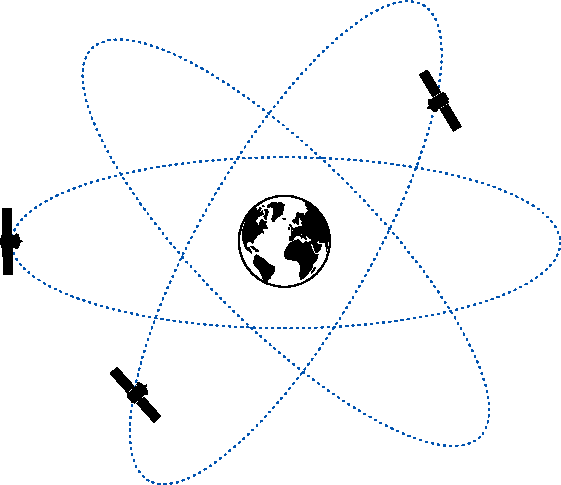
\includegraphics[width=.6\linewidth]{sat_pos}
		\captionof{figure}{Satellites de positionnement.}
	\end{center}
\end{tcb*}

\subsubsection{Satellite circumpolaires}
\begin{tcb*}[sidebyside](defi){Satellites circumpolaires}
	Ces satellites oscillent entre les pôles Nord et Sud, et ont une période
	d'environ 1h à 2h afin de balayer de nombreuses zones de la surface terrestre
	en un jour.
	\begin{itemize}
		\bitem{Orbites}~: perpendiculaires au plan équatorial, ces orbites sont
		basses (environ \SI{700}{km} de haut).
		\bitem{Mission}~: cartographier la surface terrestre de plus proche que ne
		pourrait le faire un satellite géostationnaire.
	\end{itemize}
	\tcblower
	\begin{center}
		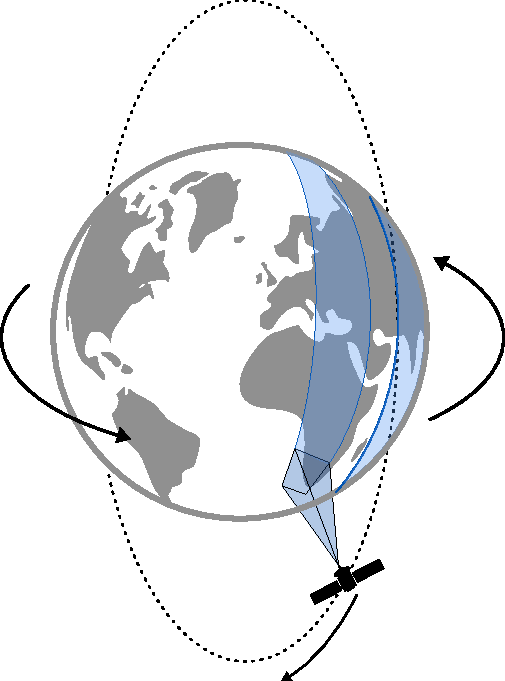
\includegraphics[width=.5\linewidth]{sat_circum}
		\captionof{figure}{Satellites circumpolaires}
	\end{center}
\end{tcb*}

\begin{tcb*}(rema)<lftt>{Sites internets}
	\begin{itemize}
		\bitem{Géostationnaires}~: \url{https://www.ssec.wisc.edu/data/geo/}
		\bitem{Circumpolaires}~:
		\begin{itemize}
			\item \url{https://earthnow.usgs.gov/observer/}
			\item \url{https://worldview.earthdata.nasa.gov}
		\end{itemize}
		\bitem{Planétarium}~: \url{https://stellarium-web.org/}
	\end{itemize}
\end{tcb*}
\end{document}
